% Capitolul 16: Rădăcini explozive și bule speculative
% Analiza avansată a seriilor de timp și previziune -- Programul de master Statistică aplicată și data science, anul I, semestrul 2, Academia de Studii Economice din București
% GENERAT de latex/build_chapter16.py -- modificați generatorul, nu acest fișier.

\newcommand{\coursename}{Analiza avansată a seriilor de timp și previziune}
\def\atslang{ro}
% Preambul comun ATS -- Analiza avansată a seriilor de timp și previziune / Advanced Time Series Analysis and Forecasting
% (Beamer, 16:9). Același design ca MFM, SFM și TSA (copiat din TSA, 5 octombrie 2026). Înainte de % Preambul comun ATS -- Analiza avansată a seriilor de timp și previziune / Advanced Time Series Analysis and Forecasting
% (Beamer, 16:9). Același design ca MFM, SFM și TSA (copiat din TSA, 5 octombrie 2026). Înainte de % Preambul comun ATS -- Analiza avansată a seriilor de timp și previziune / Advanced Time Series Analysis and Forecasting
% (Beamer, 16:9). Același design ca MFM, SFM și TSA (copiat din TSA, 5 octombrie 2026). Înainte de \input{../../latex/preamble} se definește
%   \newcommand{\coursename}{Advanced Time Series Analysis and Forecasting}          (EN)
%   \newcommand{\coursename}{Analiza avansată a seriilor de timp și previziune}       (RO)  și  \def\atslang{ro}
% Fișierele .tex se află în EN/Courses, EN/Seminars, RO/Cursuri, RO/Seminarii (două niveluri sub rădăcină).
% Deck-urile sînt generate de latex/build_chapterN.py / build_seminarN.py (vezi latex/ats_build.py).

\documentclass[9pt, aspectratio=169, t]{beamer}
\providecommand{\coursename}{Advanced Time Series Analysis and Forecasting}

% Ensure content fits on slides
\setbeamersize{text margin left=8mm, text margin right=8mm}
% Smaller institute font (title page)
\setbeamerfont{institute}{size=\footnotesize}

%=============================================================================
% THEME AND STYLE CONFIGURATION
%=============================================================================
\usetheme{default}
% Using default theme for clean header/footer control

% Color Palette (matching Redispatch PDF)
\definecolor{MainBlue}{RGB}{26, 58, 110}
\definecolor{AccentBlue}{RGB}{26, 58, 110}
\definecolor{IDAred}{RGB}{205, 0, 0}
\definecolor{DarkGray}{RGB}{51, 51, 51}
\definecolor{MediumGray}{RGB}{128, 128, 128}
\definecolor{LightGray}{RGB}{248, 248, 248}
\definecolor{VeryLightGray}{RGB}{235, 235, 235}
\definecolor{KeynoteGray}{RGB}{218, 218, 218}
\definecolor{SectionGray}{RGB}{120, 120, 120}
\definecolor{FooterGray}{RGB}{100, 100, 100}
\definecolor{Crimson}{RGB}{220, 53, 69}
\definecolor{Forest}{RGB}{46, 125, 50}
\definecolor{Amber}{RGB}{181, 133, 63}
\definecolor{Orange}{RGB}{230, 126, 34}
\definecolor{Purple}{RGB}{142, 68, 173}

% Gradient background (exact Keynote 315° gradient: white to RGB 218,218,218)
\setbeamertemplate{background}{%
    \begin{tikzpicture}[remember picture, overlay]
        \shade[shading=axis, shading angle=315,
        top color=white, bottom color=KeynoteGray]
        (current page.south west) rectangle (current page.north east);
    \end{tikzpicture}%
}
% Fallback solid color for compatibility
\setbeamercolor{background canvas}{bg=}

\setbeamercolor{palette primary}{bg=MainBlue, fg=white}
\setbeamercolor{palette secondary}{bg=MainBlue!85, fg=white}
\setbeamercolor{palette tertiary}{bg=MainBlue!70, fg=white}
\setbeamercolor{structure}{fg=MainBlue}
\setbeamercolor{title}{fg=IDAred}
\setbeamercolor{frametitle}{fg=IDAred, bg=}
\setbeamercolor{block title}{bg=MainBlue, fg=white}
\setbeamercolor{block body}{bg=VeryLightGray, fg=DarkGray}
\setbeamercolor{block title alerted}{bg=Crimson, fg=white}
\setbeamercolor{block body alerted}{bg=Crimson!8, fg=DarkGray}
\setbeamercolor{block title example}{bg=Forest, fg=white}
\setbeamercolor{block body example}{bg=Forest!8, fg=DarkGray}
\setbeamercolor{item}{fg=MainBlue}

% Footer colors (override Madrid theme blue)
\setbeamercolor{author in head/foot}{fg=FooterGray, bg=}
\setbeamercolor{title in head/foot}{fg=FooterGray, bg=}
\setbeamercolor{date in head/foot}{fg=FooterGray, bg=}
\setbeamercolor{section in head/foot}{fg=FooterGray, bg=}
\setbeamercolor{subsection in head/foot}{fg=FooterGray, bg=}

% Bullet styles (apply everywhere including blocks)
\setbeamertemplate{itemize item}{\color{MainBlue}$\boxdot$}
\setbeamertemplate{itemize subitem}{\color{MainBlue}$\blacktriangleright$}
\setbeamertemplate{itemize subsubitem}{\color{MainBlue}\tiny$\bullet$}
\setbeamertemplate{itemize/enumerate body begin}{\normalsize}
\setbeamertemplate{itemize/enumerate subbody begin}{\normalsize}

% Item spacing - compact style
\setlength{\leftmargini}{10pt}       % Level 1: minimal indent
\setlength{\leftmarginii}{10pt}      % Level 2: minimal additional indent
% Compact list spacing (zero extra space before/after lists in blocks)
\makeatletter
\def\@listi{\leftmargin\leftmargini \topsep 0pt \parsep 0pt \itemsep 0pt}
\def\@listii{\leftmargin\leftmarginii \topsep 0pt \parsep 0pt \itemsep 0pt}
\makeatother

\setbeamertemplate{navigation symbols}{}

%=============================================================================
% CUSTOM HEADLINE
%=============================================================================
\setbeamertemplate{headline}{%
    \vskip10pt%
    \hbox to \paperwidth{%
        \hskip0.5cm%
        {\small\color{FooterGray}\renewcommand{\hyperlink}[2]{##2}\insertsectionhead}%
        \hfill%
        \textcolor{FooterGray}{\small\insertframenumber}%
        \hskip0.5cm%
    }%
    \vskip4pt%
    {\color{FooterGray}\hrule height 0.4pt}%
}

%=============================================================================
% CUSTOM FOOTER
%=============================================================================
\usepackage{fontawesome5}

\setbeamertemplate{footline}{%
    {\color{FooterGray}\hrule height 0.4pt}%
    \vskip4pt%
    \hbox to \paperwidth{%
        \hskip0.5cm%
        \textcolor{FooterGray}{\small\coursename}%
        \hfill%
        \raisebox{-0.1em}{%
            \begin{tikzpicture}[x=0.08em, y=0.08em, line width=0.4pt]
                \draw[FooterGray] (0,3) -- (1,4) -- (2,3.5) -- (3,5) -- (4,4) -- (5,6) -- (6,5.5) -- (7,4) -- (8,5) -- (9,7) -- (10,6) -- (11,5) -- (12,6.5) -- (13,8) -- (14,7) -- (15,6) -- (16,7.5) -- (17,9) -- (18,8) -- (19,7) -- (20,8.5) -- (21,10) -- (22,9) -- (23,8) -- (24,9.5);
            \end{tikzpicture}%
        }%
        \hskip0.5cm%
    }%
    \vskip6pt%
}

%=============================================================================
% PACKAGES
%=============================================================================
\usepackage[utf8]{inputenc}
\DeclareUnicodeCharacter{03B1}{\ensuremath{\alpha}}
\usepackage[T1]{fontenc}
\usepackage{amsmath, amssymb, amsthm}
\usepackage{mathtools}
\usepackage{bm}
\usepackage{tikz}
\usetikzlibrary{arrows.meta, positioning, shapes, calc, decorations.pathreplacing, shadings}
\usepackage{booktabs}
\usepackage{multirow}
\usepackage{array}
\usepackage{graphicx}
\usepackage{animate}
\usepackage{hyperref}
\usepackage{colortbl}
\usepackage{listings}
\lstset{language=Python, basicstyle=\ttfamily\scriptsize, keywordstyle=\color{MainBlue}\bfseries,
  commentstyle=\color{Forest}, stringstyle=\color{Crimson}, breaklines=true,
  frame=none, backgroundcolor=\color{VeryLightGray}, xleftmargin=2mm}
\hypersetup{colorlinks=true, linkcolor=MainBlue, urlcolor=MainBlue}
\graphicspath{{../../logos/}{../../charts/}{../../photos/}}
\usepackage{xcolor}
\hfuzz=2pt  % Suppress tiny overfull warnings (<2pt)
\vfuzz=2pt  % Suppress tiny vertical overfull warnings (<2pt)

%=============================================================================
% QUANTLET COMMANDS
%   \quantlet{<displayed name>}{<url>}       (generic)
%   \atsquantlet{Ch_05}{ATS_ch5_garch}       -> https://github.com/danpele/Advanced-Time-Series/tree/main/Quantlets/Ch_05/ATS_ch5_garch
%   \qlurl{<folder>} is defined per chapter by the generator (Quantlets/Ch_NN/<folder>)
%=============================================================================
\newcommand{\atsrepo}{https://github.com/danpele/Advanced-Time-Series}
\newcommand{\atsqlbase}{https://github.com/danpele/Advanced-Time-Series/tree/main/Quantlets}
\newcommand{\quantlet}[2]{%
    \hfill\href{#2}{%
        \raisebox{-0.15em}{
\includegraphics[height=0.7em]{ql_logo.png}}%
        \textcolor{MainBlue}{\tiny\ #1}%
    }%
}
\newcommand{\atsquantlet}[2]{\quantlet{\detokenize{#2}}{\atsqlbase/#1/#2}}

%=============================================================================
% NOTEBOOKS (Google Colab)
%   \colaburl{notebooks/EN/chapter5_seminar_notebook.ipynb} -> the Colab link of a file in the ATS repo
%   \nb: the chapter notebook (each seminar deck redefines it with \renewcommand)
%=============================================================================
\newcommand{\colaburl}[1]{https://colab.research.google.com/github/danpele/Advanced-Time-Series/blob/main/#1}
\newcommand{\nb}{https://colab.research.google.com/github/danpele/Advanced-Time-Series/tree/main/notebooks/EN}
\newcommand{\nbname}{notebooks/EN}

%=============================================================================
% SLIDE HELPERS (used by the generators; the same as in MFM)
%=============================================================================
% local font size for list bodies (the preamble forces \normalsize)
\newcommand{\itemsize}[1]{\setbeamertemplate{itemize/enumerate body begin}{#1}\setbeamertemplate{itemize/enumerate subbody begin}{#1}}
\newcommand{\intitle}[1]{{\hypersetup{urlcolor=white}#1}}   % white links inside coloured title bars
\newcommand{\imgcap}[1]{{\scriptsize #1}\\[0.5mm]}          % caption under a photo
\newcommand{\imgcredit}[2]{{\tiny\color{FooterGray}\href{#1}{#2}}}   % image credit: source URL, author/licence
\newcommand{\aiprompt}[1]{{\ttfamily\color{MainBlue}#1}}     % a prompt to an AI assistant

%=============================================================================
% SEMINARS: student version by default; the instructor wrapper *_solutions.tex sets \solutionstrue
%=============================================================================
\makeatletter\@ifundefined{ifsolutions}{\expandafter\newif\csname ifsolutions\endcsname}{}\makeatother
\newcommand{\solonly}[1]{\ifsolutions #1\fi}
\newcommand{\propsub}{\ifsolutions\else\framesubtitle{\ifdefined\atslang Rezolvarea se discută la seminar\else Solution discussed in class\fi}\fi}

%=============================================================================
% APPENDIX AND CHAPTER LINKS (latex/appendix_links.py writes the calls; it also re-declares these
% macros before \begin{document}, so the decks compile with or without this preamble block)
%=============================================================================
\providecommand{\atsapplink}[3]{\hypertarget{#2}{}\hyperlink{#1}{\beamergotobutton{#3}}}
\providecommand{\atsappback}[2]{\begin{tikzpicture}[remember picture,overlay]\node[anchor=south east] at ([xshift=-3mm,yshift=7mm]current page.south east){\hyperlink{#1}{\beamerreturnbutton{#2}}};\end{tikzpicture}}
\providecommand{\atschlink}[2]{\href{#1}{#2}}
\providecommand{\atschlinkt}[2]{\href{#1}{\usebeamercolor[fg]{frametitle}#2}}

%=============================================================================
% QUANTINAR COMMAND: link către un curs Quantinar (subiecte avansate)
%=============================================================================
\newcommand{\quantinar}[2]{%
    \href{#2}{%
        \raisebox{-0.15em}{
\includegraphics[height=0.8em]{qr_logo.png}}%
        \textcolor{MainBlue}{\scriptsize\ #1}%
    }%
}

%=============================================================================
% CUSTOM TITLE PAGE
%=============================================================================
\defbeamertemplate*{title page}{hybrid}[1][]
{
    \vspace{0.2cm}
    % Logos row - top header (with clickable links)
    \begin{center}
        \href{https://www.ase.ro}{
\includegraphics[height=1.0cm]{ase_logo.png}}\hspace{0.3cm}%
        \href{https://theida.net}{
\includegraphics[height=1.0cm]{ida_logo.png}}\hspace{0.3cm}%
        \href{https://blockchain-research-center.com}{
\includegraphics[height=1.0cm]{brc_logo.png}}\hspace{0.3cm}%
        \href{https://www.ai4efin.ase.ro}{
\includegraphics[height=1.0cm]{ai4efin_logo.png}}\hspace{0.3cm}%
        \href{https://ipe.ro/new}{
\includegraphics[height=1.0cm]{acad_logo.png}}\hspace{0.3cm}%
        \href{https://www.digital-finance-msca.com}{
\includegraphics[height=1.0cm]{msca_logo.png}}%
    \end{center}

    \vspace{0.6cm}

    % Main title with Q logos on sides (with clickable links)
    \begin{center}
        \begin{minipage}{0.1\textwidth}
            \centering
            \href{https://quantlet.com}{
\includegraphics[height=1.1cm]{ql_logo.png}}
        \end{minipage}%
        \begin{minipage}{0.78\textwidth}
            \centering
            {\LARGE\bfseries\usebeamercolor[fg]{title}\inserttitle}

            \vspace{0.3cm}

            {\usebeamerfont{subtitle}\usebeamercolor[fg]{title}\insertsubtitle}
        \end{minipage}%
        \begin{minipage}{0.1\textwidth}
            \centering
            \href{https://quantinar.com}{
\includegraphics[height=1.1cm]{qr_logo.png}}
        \end{minipage}
    \end{center}

    \vspace{0.6cm}

    % Authors (left aligned)
    \hspace{0.5cm}{\usebeamerfont{author}\insertauthor}

    \vspace{0.3cm}

    % Institute/Affiliations (left aligned)
    \hspace{0.5cm}\begin{minipage}[t]{0.9\textwidth}
        \raggedright\small\insertinstitute
    \end{minipage}
}

%=============================================================================
% THEOREM ENVIRONMENTS
%=============================================================================
\theoremstyle{definition}
\setbeamertemplate{theorems}[numbered]
\ifdefined\atslang
\newtheorem{defn}{Definiție}
\newtheorem{thm}{Teoremă}
\newtheorem{prop}{Propoziție}
\newtheorem{rmk}{Observație}
\else
\newtheorem{defn}{Definition}
\newtheorem{thm}{Theorem}
\newtheorem{prop}{Proposition}
\newtheorem{rmk}{Remark}
\fi

%=============================================================================
% CENTRED MINIPAGE (no extra vertical space)
%=============================================================================
\newenvironment{cminipage}[1]{%
    \par\noindent\hfill\begin{minipage}{#1}\ignorespaces
}{%
    \end{minipage}\hfill\null\par
}

%=============================================================================
% CUSTOM COMMANDS
%=============================================================================
\newcommand{\E}{\mathbb{E}}
\newcommand{\Var}{\text{Var}}
\newcommand{\Cov}{\text{Cov}}
\newcommand{\Corr}{\text{Corr}}
\newcommand{\R}{\mathbb{R}}
\newcommand{\N}{\mathbb{N}}
\newcommand{\Z}{\mathbb{Z}}
\newcommand{\B}{\mathbf{B}}
\newcommand{\imark}{\textcolor{MainBlue}{\textbullet}}
\newcommand{\RMSE}{\text{RMSE}}
\newcommand{\MAE}{\text{MAE}}
\newcommand{\MAPE}{\text{MAPE}}

% Boldface vector/matrix commands (VAR, VECM, state space)
\newcommand{\bY}{\mathbf{Y}}
\newcommand{\bX}{\mathbf{X}}
\newcommand{\bA}{\mathbf{A}}
\newcommand{\bB}{\mathbf{B}}
\newcommand{\bepsilon}{\boldsymbol{\varepsilon}}
\newcommand{\bSigma}{\boldsymbol{\Sigma}}
\newcommand{\bPhi}{\boldsymbol{\Phi}}
\newcommand{\bGamma}{\boldsymbol{\Gamma}}
\newcommand{\bPi}{\boldsymbol{\Pi}}
\newcommand{\bc}{\mathbf{c}}
\newcommand{\balpha}{\boldsymbol{\alpha}}
\newcommand{\bbeta}{\boldsymbol{\beta}}
\newcommand{\bvarepsilon}{\boldsymbol{\varepsilon}}

% Seminar marks
\newcommand{\correct}{\textcolor{Forest}{\checkmark}}
\newcommand{\incorrect}{\textcolor{Crimson}{\texttimes}}
 se definește
%   \newcommand{\coursename}{Advanced Time Series Analysis and Forecasting}          (EN)
%   \newcommand{\coursename}{Analiza avansată a seriilor de timp și previziune}       (RO)  și  \def\atslang{ro}
% Fișierele .tex se află în EN/Courses, EN/Seminars, RO/Cursuri, RO/Seminarii (două niveluri sub rădăcină).
% Deck-urile sînt generate de latex/build_chapterN.py / build_seminarN.py (vezi latex/ats_build.py).

\documentclass[9pt, aspectratio=169, t]{beamer}
\providecommand{\coursename}{Advanced Time Series Analysis and Forecasting}

% Ensure content fits on slides
\setbeamersize{text margin left=8mm, text margin right=8mm}
% Smaller institute font (title page)
\setbeamerfont{institute}{size=\footnotesize}

%=============================================================================
% THEME AND STYLE CONFIGURATION
%=============================================================================
\usetheme{default}
% Using default theme for clean header/footer control

% Color Palette (matching Redispatch PDF)
\definecolor{MainBlue}{RGB}{26, 58, 110}
\definecolor{AccentBlue}{RGB}{26, 58, 110}
\definecolor{IDAred}{RGB}{205, 0, 0}
\definecolor{DarkGray}{RGB}{51, 51, 51}
\definecolor{MediumGray}{RGB}{128, 128, 128}
\definecolor{LightGray}{RGB}{248, 248, 248}
\definecolor{VeryLightGray}{RGB}{235, 235, 235}
\definecolor{KeynoteGray}{RGB}{218, 218, 218}
\definecolor{SectionGray}{RGB}{120, 120, 120}
\definecolor{FooterGray}{RGB}{100, 100, 100}
\definecolor{Crimson}{RGB}{220, 53, 69}
\definecolor{Forest}{RGB}{46, 125, 50}
\definecolor{Amber}{RGB}{181, 133, 63}
\definecolor{Orange}{RGB}{230, 126, 34}
\definecolor{Purple}{RGB}{142, 68, 173}

% Gradient background (exact Keynote 315° gradient: white to RGB 218,218,218)
\setbeamertemplate{background}{%
    \begin{tikzpicture}[remember picture, overlay]
        \shade[shading=axis, shading angle=315,
        top color=white, bottom color=KeynoteGray]
        (current page.south west) rectangle (current page.north east);
    \end{tikzpicture}%
}
% Fallback solid color for compatibility
\setbeamercolor{background canvas}{bg=}

\setbeamercolor{palette primary}{bg=MainBlue, fg=white}
\setbeamercolor{palette secondary}{bg=MainBlue!85, fg=white}
\setbeamercolor{palette tertiary}{bg=MainBlue!70, fg=white}
\setbeamercolor{structure}{fg=MainBlue}
\setbeamercolor{title}{fg=IDAred}
\setbeamercolor{frametitle}{fg=IDAred, bg=}
\setbeamercolor{block title}{bg=MainBlue, fg=white}
\setbeamercolor{block body}{bg=VeryLightGray, fg=DarkGray}
\setbeamercolor{block title alerted}{bg=Crimson, fg=white}
\setbeamercolor{block body alerted}{bg=Crimson!8, fg=DarkGray}
\setbeamercolor{block title example}{bg=Forest, fg=white}
\setbeamercolor{block body example}{bg=Forest!8, fg=DarkGray}
\setbeamercolor{item}{fg=MainBlue}

% Footer colors (override Madrid theme blue)
\setbeamercolor{author in head/foot}{fg=FooterGray, bg=}
\setbeamercolor{title in head/foot}{fg=FooterGray, bg=}
\setbeamercolor{date in head/foot}{fg=FooterGray, bg=}
\setbeamercolor{section in head/foot}{fg=FooterGray, bg=}
\setbeamercolor{subsection in head/foot}{fg=FooterGray, bg=}

% Bullet styles (apply everywhere including blocks)
\setbeamertemplate{itemize item}{\color{MainBlue}$\boxdot$}
\setbeamertemplate{itemize subitem}{\color{MainBlue}$\blacktriangleright$}
\setbeamertemplate{itemize subsubitem}{\color{MainBlue}\tiny$\bullet$}
\setbeamertemplate{itemize/enumerate body begin}{\normalsize}
\setbeamertemplate{itemize/enumerate subbody begin}{\normalsize}

% Item spacing - compact style
\setlength{\leftmargini}{10pt}       % Level 1: minimal indent
\setlength{\leftmarginii}{10pt}      % Level 2: minimal additional indent
% Compact list spacing (zero extra space before/after lists in blocks)
\makeatletter
\def\@listi{\leftmargin\leftmargini \topsep 0pt \parsep 0pt \itemsep 0pt}
\def\@listii{\leftmargin\leftmarginii \topsep 0pt \parsep 0pt \itemsep 0pt}
\makeatother

\setbeamertemplate{navigation symbols}{}

%=============================================================================
% CUSTOM HEADLINE
%=============================================================================
\setbeamertemplate{headline}{%
    \vskip10pt%
    \hbox to \paperwidth{%
        \hskip0.5cm%
        {\small\color{FooterGray}\renewcommand{\hyperlink}[2]{##2}\insertsectionhead}%
        \hfill%
        \textcolor{FooterGray}{\small\insertframenumber}%
        \hskip0.5cm%
    }%
    \vskip4pt%
    {\color{FooterGray}\hrule height 0.4pt}%
}

%=============================================================================
% CUSTOM FOOTER
%=============================================================================
\usepackage{fontawesome5}

\setbeamertemplate{footline}{%
    {\color{FooterGray}\hrule height 0.4pt}%
    \vskip4pt%
    \hbox to \paperwidth{%
        \hskip0.5cm%
        \textcolor{FooterGray}{\small\coursename}%
        \hfill%
        \raisebox{-0.1em}{%
            \begin{tikzpicture}[x=0.08em, y=0.08em, line width=0.4pt]
                \draw[FooterGray] (0,3) -- (1,4) -- (2,3.5) -- (3,5) -- (4,4) -- (5,6) -- (6,5.5) -- (7,4) -- (8,5) -- (9,7) -- (10,6) -- (11,5) -- (12,6.5) -- (13,8) -- (14,7) -- (15,6) -- (16,7.5) -- (17,9) -- (18,8) -- (19,7) -- (20,8.5) -- (21,10) -- (22,9) -- (23,8) -- (24,9.5);
            \end{tikzpicture}%
        }%
        \hskip0.5cm%
    }%
    \vskip6pt%
}

%=============================================================================
% PACKAGES
%=============================================================================
\usepackage[utf8]{inputenc}
\DeclareUnicodeCharacter{03B1}{\ensuremath{\alpha}}
\usepackage[T1]{fontenc}
\usepackage{amsmath, amssymb, amsthm}
\usepackage{mathtools}
\usepackage{bm}
\usepackage{tikz}
\usetikzlibrary{arrows.meta, positioning, shapes, calc, decorations.pathreplacing, shadings}
\usepackage{booktabs}
\usepackage{multirow}
\usepackage{array}
\usepackage{graphicx}
\usepackage{animate}
\usepackage{hyperref}
\usepackage{colortbl}
\usepackage{listings}
\lstset{language=Python, basicstyle=\ttfamily\scriptsize, keywordstyle=\color{MainBlue}\bfseries,
  commentstyle=\color{Forest}, stringstyle=\color{Crimson}, breaklines=true,
  frame=none, backgroundcolor=\color{VeryLightGray}, xleftmargin=2mm}
\hypersetup{colorlinks=true, linkcolor=MainBlue, urlcolor=MainBlue}
\graphicspath{{../../logos/}{../../charts/}{../../photos/}}
\usepackage{xcolor}
\hfuzz=2pt  % Suppress tiny overfull warnings (<2pt)
\vfuzz=2pt  % Suppress tiny vertical overfull warnings (<2pt)

%=============================================================================
% QUANTLET COMMANDS
%   \quantlet{<displayed name>}{<url>}       (generic)
%   \atsquantlet{Ch_05}{ATS_ch5_garch}       -> https://github.com/danpele/Advanced-Time-Series/tree/main/Quantlets/Ch_05/ATS_ch5_garch
%   \qlurl{<folder>} is defined per chapter by the generator (Quantlets/Ch_NN/<folder>)
%=============================================================================
\newcommand{\atsrepo}{https://github.com/danpele/Advanced-Time-Series}
\newcommand{\atsqlbase}{https://github.com/danpele/Advanced-Time-Series/tree/main/Quantlets}
\newcommand{\quantlet}[2]{%
    \hfill\href{#2}{%
        \raisebox{-0.15em}{
\includegraphics[height=0.7em]{ql_logo.png}}%
        \textcolor{MainBlue}{\tiny\ #1}%
    }%
}
\newcommand{\atsquantlet}[2]{\quantlet{\detokenize{#2}}{\atsqlbase/#1/#2}}

%=============================================================================
% NOTEBOOKS (Google Colab)
%   \colaburl{notebooks/EN/chapter5_seminar_notebook.ipynb} -> the Colab link of a file in the ATS repo
%   \nb: the chapter notebook (each seminar deck redefines it with \renewcommand)
%=============================================================================
\newcommand{\colaburl}[1]{https://colab.research.google.com/github/danpele/Advanced-Time-Series/blob/main/#1}
\newcommand{\nb}{https://colab.research.google.com/github/danpele/Advanced-Time-Series/tree/main/notebooks/EN}
\newcommand{\nbname}{notebooks/EN}

%=============================================================================
% SLIDE HELPERS (used by the generators; the same as in MFM)
%=============================================================================
% local font size for list bodies (the preamble forces \normalsize)
\newcommand{\itemsize}[1]{\setbeamertemplate{itemize/enumerate body begin}{#1}\setbeamertemplate{itemize/enumerate subbody begin}{#1}}
\newcommand{\intitle}[1]{{\hypersetup{urlcolor=white}#1}}   % white links inside coloured title bars
\newcommand{\imgcap}[1]{{\scriptsize #1}\\[0.5mm]}          % caption under a photo
\newcommand{\imgcredit}[2]{{\tiny\color{FooterGray}\href{#1}{#2}}}   % image credit: source URL, author/licence
\newcommand{\aiprompt}[1]{{\ttfamily\color{MainBlue}#1}}     % a prompt to an AI assistant

%=============================================================================
% SEMINARS: student version by default; the instructor wrapper *_solutions.tex sets \solutionstrue
%=============================================================================
\makeatletter\@ifundefined{ifsolutions}{\expandafter\newif\csname ifsolutions\endcsname}{}\makeatother
\newcommand{\solonly}[1]{\ifsolutions #1\fi}
\newcommand{\propsub}{\ifsolutions\else\framesubtitle{\ifdefined\atslang Rezolvarea se discută la seminar\else Solution discussed in class\fi}\fi}

%=============================================================================
% APPENDIX AND CHAPTER LINKS (latex/appendix_links.py writes the calls; it also re-declares these
% macros before \begin{document}, so the decks compile with or without this preamble block)
%=============================================================================
\providecommand{\atsapplink}[3]{\hypertarget{#2}{}\hyperlink{#1}{\beamergotobutton{#3}}}
\providecommand{\atsappback}[2]{\begin{tikzpicture}[remember picture,overlay]\node[anchor=south east] at ([xshift=-3mm,yshift=7mm]current page.south east){\hyperlink{#1}{\beamerreturnbutton{#2}}};\end{tikzpicture}}
\providecommand{\atschlink}[2]{\href{#1}{#2}}
\providecommand{\atschlinkt}[2]{\href{#1}{\usebeamercolor[fg]{frametitle}#2}}

%=============================================================================
% QUANTINAR COMMAND: link către un curs Quantinar (subiecte avansate)
%=============================================================================
\newcommand{\quantinar}[2]{%
    \href{#2}{%
        \raisebox{-0.15em}{
\includegraphics[height=0.8em]{qr_logo.png}}%
        \textcolor{MainBlue}{\scriptsize\ #1}%
    }%
}

%=============================================================================
% CUSTOM TITLE PAGE
%=============================================================================
\defbeamertemplate*{title page}{hybrid}[1][]
{
    \vspace{0.2cm}
    % Logos row - top header (with clickable links)
    \begin{center}
        \href{https://www.ase.ro}{
\includegraphics[height=1.0cm]{ase_logo.png}}\hspace{0.3cm}%
        \href{https://theida.net}{
\includegraphics[height=1.0cm]{ida_logo.png}}\hspace{0.3cm}%
        \href{https://blockchain-research-center.com}{
\includegraphics[height=1.0cm]{brc_logo.png}}\hspace{0.3cm}%
        \href{https://www.ai4efin.ase.ro}{
\includegraphics[height=1.0cm]{ai4efin_logo.png}}\hspace{0.3cm}%
        \href{https://ipe.ro/new}{
\includegraphics[height=1.0cm]{acad_logo.png}}\hspace{0.3cm}%
        \href{https://www.digital-finance-msca.com}{
\includegraphics[height=1.0cm]{msca_logo.png}}%
    \end{center}

    \vspace{0.6cm}

    % Main title with Q logos on sides (with clickable links)
    \begin{center}
        \begin{minipage}{0.1\textwidth}
            \centering
            \href{https://quantlet.com}{
\includegraphics[height=1.1cm]{ql_logo.png}}
        \end{minipage}%
        \begin{minipage}{0.78\textwidth}
            \centering
            {\LARGE\bfseries\usebeamercolor[fg]{title}\inserttitle}

            \vspace{0.3cm}

            {\usebeamerfont{subtitle}\usebeamercolor[fg]{title}\insertsubtitle}
        \end{minipage}%
        \begin{minipage}{0.1\textwidth}
            \centering
            \href{https://quantinar.com}{
\includegraphics[height=1.1cm]{qr_logo.png}}
        \end{minipage}
    \end{center}

    \vspace{0.6cm}

    % Authors (left aligned)
    \hspace{0.5cm}{\usebeamerfont{author}\insertauthor}

    \vspace{0.3cm}

    % Institute/Affiliations (left aligned)
    \hspace{0.5cm}\begin{minipage}[t]{0.9\textwidth}
        \raggedright\small\insertinstitute
    \end{minipage}
}

%=============================================================================
% THEOREM ENVIRONMENTS
%=============================================================================
\theoremstyle{definition}
\setbeamertemplate{theorems}[numbered]
\ifdefined\atslang
\newtheorem{defn}{Definiție}
\newtheorem{thm}{Teoremă}
\newtheorem{prop}{Propoziție}
\newtheorem{rmk}{Observație}
\else
\newtheorem{defn}{Definition}
\newtheorem{thm}{Theorem}
\newtheorem{prop}{Proposition}
\newtheorem{rmk}{Remark}
\fi

%=============================================================================
% CENTRED MINIPAGE (no extra vertical space)
%=============================================================================
\newenvironment{cminipage}[1]{%
    \par\noindent\hfill\begin{minipage}{#1}\ignorespaces
}{%
    \end{minipage}\hfill\null\par
}

%=============================================================================
% CUSTOM COMMANDS
%=============================================================================
\newcommand{\E}{\mathbb{E}}
\newcommand{\Var}{\text{Var}}
\newcommand{\Cov}{\text{Cov}}
\newcommand{\Corr}{\text{Corr}}
\newcommand{\R}{\mathbb{R}}
\newcommand{\N}{\mathbb{N}}
\newcommand{\Z}{\mathbb{Z}}
\newcommand{\B}{\mathbf{B}}
\newcommand{\imark}{\textcolor{MainBlue}{\textbullet}}
\newcommand{\RMSE}{\text{RMSE}}
\newcommand{\MAE}{\text{MAE}}
\newcommand{\MAPE}{\text{MAPE}}

% Boldface vector/matrix commands (VAR, VECM, state space)
\newcommand{\bY}{\mathbf{Y}}
\newcommand{\bX}{\mathbf{X}}
\newcommand{\bA}{\mathbf{A}}
\newcommand{\bB}{\mathbf{B}}
\newcommand{\bepsilon}{\boldsymbol{\varepsilon}}
\newcommand{\bSigma}{\boldsymbol{\Sigma}}
\newcommand{\bPhi}{\boldsymbol{\Phi}}
\newcommand{\bGamma}{\boldsymbol{\Gamma}}
\newcommand{\bPi}{\boldsymbol{\Pi}}
\newcommand{\bc}{\mathbf{c}}
\newcommand{\balpha}{\boldsymbol{\alpha}}
\newcommand{\bbeta}{\boldsymbol{\beta}}
\newcommand{\bvarepsilon}{\boldsymbol{\varepsilon}}

% Seminar marks
\newcommand{\correct}{\textcolor{Forest}{\checkmark}}
\newcommand{\incorrect}{\textcolor{Crimson}{\texttimes}}
 se definește
%   \newcommand{\coursename}{Advanced Time Series Analysis and Forecasting}          (EN)
%   \newcommand{\coursename}{Analiza avansată a seriilor de timp și previziune}       (RO)  și  \def\atslang{ro}
% Fișierele .tex se află în EN/Courses, EN/Seminars, RO/Cursuri, RO/Seminarii (două niveluri sub rădăcină).
% Deck-urile sînt generate de latex/build_chapterN.py / build_seminarN.py (vezi latex/ats_build.py).

\documentclass[9pt, aspectratio=169, t]{beamer}
\providecommand{\coursename}{Advanced Time Series Analysis and Forecasting}

% Ensure content fits on slides
\setbeamersize{text margin left=8mm, text margin right=8mm}
% Smaller institute font (title page)
\setbeamerfont{institute}{size=\footnotesize}

%=============================================================================
% THEME AND STYLE CONFIGURATION
%=============================================================================
\usetheme{default}
% Using default theme for clean header/footer control

% Color Palette (matching Redispatch PDF)
\definecolor{MainBlue}{RGB}{26, 58, 110}
\definecolor{AccentBlue}{RGB}{26, 58, 110}
\definecolor{IDAred}{RGB}{205, 0, 0}
\definecolor{DarkGray}{RGB}{51, 51, 51}
\definecolor{MediumGray}{RGB}{128, 128, 128}
\definecolor{LightGray}{RGB}{248, 248, 248}
\definecolor{VeryLightGray}{RGB}{235, 235, 235}
\definecolor{KeynoteGray}{RGB}{218, 218, 218}
\definecolor{SectionGray}{RGB}{120, 120, 120}
\definecolor{FooterGray}{RGB}{100, 100, 100}
\definecolor{Crimson}{RGB}{220, 53, 69}
\definecolor{Forest}{RGB}{46, 125, 50}
\definecolor{Amber}{RGB}{181, 133, 63}
\definecolor{Orange}{RGB}{230, 126, 34}
\definecolor{Purple}{RGB}{142, 68, 173}

% Gradient background (exact Keynote 315° gradient: white to RGB 218,218,218)
\setbeamertemplate{background}{%
    \begin{tikzpicture}[remember picture, overlay]
        \shade[shading=axis, shading angle=315,
        top color=white, bottom color=KeynoteGray]
        (current page.south west) rectangle (current page.north east);
    \end{tikzpicture}%
}
% Fallback solid color for compatibility
\setbeamercolor{background canvas}{bg=}

\setbeamercolor{palette primary}{bg=MainBlue, fg=white}
\setbeamercolor{palette secondary}{bg=MainBlue!85, fg=white}
\setbeamercolor{palette tertiary}{bg=MainBlue!70, fg=white}
\setbeamercolor{structure}{fg=MainBlue}
\setbeamercolor{title}{fg=IDAred}
\setbeamercolor{frametitle}{fg=IDAred, bg=}
\setbeamercolor{block title}{bg=MainBlue, fg=white}
\setbeamercolor{block body}{bg=VeryLightGray, fg=DarkGray}
\setbeamercolor{block title alerted}{bg=Crimson, fg=white}
\setbeamercolor{block body alerted}{bg=Crimson!8, fg=DarkGray}
\setbeamercolor{block title example}{bg=Forest, fg=white}
\setbeamercolor{block body example}{bg=Forest!8, fg=DarkGray}
\setbeamercolor{item}{fg=MainBlue}

% Footer colors (override Madrid theme blue)
\setbeamercolor{author in head/foot}{fg=FooterGray, bg=}
\setbeamercolor{title in head/foot}{fg=FooterGray, bg=}
\setbeamercolor{date in head/foot}{fg=FooterGray, bg=}
\setbeamercolor{section in head/foot}{fg=FooterGray, bg=}
\setbeamercolor{subsection in head/foot}{fg=FooterGray, bg=}

% Bullet styles (apply everywhere including blocks)
\setbeamertemplate{itemize item}{\color{MainBlue}$\boxdot$}
\setbeamertemplate{itemize subitem}{\color{MainBlue}$\blacktriangleright$}
\setbeamertemplate{itemize subsubitem}{\color{MainBlue}\tiny$\bullet$}
\setbeamertemplate{itemize/enumerate body begin}{\normalsize}
\setbeamertemplate{itemize/enumerate subbody begin}{\normalsize}

% Item spacing - compact style
\setlength{\leftmargini}{10pt}       % Level 1: minimal indent
\setlength{\leftmarginii}{10pt}      % Level 2: minimal additional indent
% Compact list spacing (zero extra space before/after lists in blocks)
\makeatletter
\def\@listi{\leftmargin\leftmargini \topsep 0pt \parsep 0pt \itemsep 0pt}
\def\@listii{\leftmargin\leftmarginii \topsep 0pt \parsep 0pt \itemsep 0pt}
\makeatother

\setbeamertemplate{navigation symbols}{}

%=============================================================================
% CUSTOM HEADLINE
%=============================================================================
\setbeamertemplate{headline}{%
    \vskip10pt%
    \hbox to \paperwidth{%
        \hskip0.5cm%
        {\small\color{FooterGray}\renewcommand{\hyperlink}[2]{##2}\insertsectionhead}%
        \hfill%
        \textcolor{FooterGray}{\small\insertframenumber}%
        \hskip0.5cm%
    }%
    \vskip4pt%
    {\color{FooterGray}\hrule height 0.4pt}%
}

%=============================================================================
% CUSTOM FOOTER
%=============================================================================
\usepackage{fontawesome5}

\setbeamertemplate{footline}{%
    {\color{FooterGray}\hrule height 0.4pt}%
    \vskip4pt%
    \hbox to \paperwidth{%
        \hskip0.5cm%
        \textcolor{FooterGray}{\small\coursename}%
        \hfill%
        \raisebox{-0.1em}{%
            \begin{tikzpicture}[x=0.08em, y=0.08em, line width=0.4pt]
                \draw[FooterGray] (0,3) -- (1,4) -- (2,3.5) -- (3,5) -- (4,4) -- (5,6) -- (6,5.5) -- (7,4) -- (8,5) -- (9,7) -- (10,6) -- (11,5) -- (12,6.5) -- (13,8) -- (14,7) -- (15,6) -- (16,7.5) -- (17,9) -- (18,8) -- (19,7) -- (20,8.5) -- (21,10) -- (22,9) -- (23,8) -- (24,9.5);
            \end{tikzpicture}%
        }%
        \hskip0.5cm%
    }%
    \vskip6pt%
}

%=============================================================================
% PACKAGES
%=============================================================================
\usepackage[utf8]{inputenc}
\DeclareUnicodeCharacter{03B1}{\ensuremath{\alpha}}
\usepackage[T1]{fontenc}
\usepackage{amsmath, amssymb, amsthm}
\usepackage{mathtools}
\usepackage{bm}
\usepackage{tikz}
\usetikzlibrary{arrows.meta, positioning, shapes, calc, decorations.pathreplacing, shadings}
\usepackage{booktabs}
\usepackage{multirow}
\usepackage{array}
\usepackage{graphicx}
\usepackage{animate}
\usepackage{hyperref}
\usepackage{colortbl}
\usepackage{listings}
\lstset{language=Python, basicstyle=\ttfamily\scriptsize, keywordstyle=\color{MainBlue}\bfseries,
  commentstyle=\color{Forest}, stringstyle=\color{Crimson}, breaklines=true,
  frame=none, backgroundcolor=\color{VeryLightGray}, xleftmargin=2mm}
\hypersetup{colorlinks=true, linkcolor=MainBlue, urlcolor=MainBlue}
\graphicspath{{../../logos/}{../../charts/}{../../photos/}}
\usepackage{xcolor}
\hfuzz=2pt  % Suppress tiny overfull warnings (<2pt)
\vfuzz=2pt  % Suppress tiny vertical overfull warnings (<2pt)

%=============================================================================
% QUANTLET COMMANDS
%   \quantlet{<displayed name>}{<url>}       (generic)
%   \atsquantlet{Ch_05}{ATS_ch5_garch}       -> https://github.com/danpele/Advanced-Time-Series/tree/main/Quantlets/Ch_05/ATS_ch5_garch
%   \qlurl{<folder>} is defined per chapter by the generator (Quantlets/Ch_NN/<folder>)
%=============================================================================
\newcommand{\atsrepo}{https://github.com/danpele/Advanced-Time-Series}
\newcommand{\atsqlbase}{https://github.com/danpele/Advanced-Time-Series/tree/main/Quantlets}
\newcommand{\quantlet}[2]{%
    \hfill\href{#2}{%
        \raisebox{-0.15em}{
\includegraphics[height=0.7em]{ql_logo.png}}%
        \textcolor{MainBlue}{\tiny\ #1}%
    }%
}
\newcommand{\atsquantlet}[2]{\quantlet{\detokenize{#2}}{\atsqlbase/#1/#2}}

%=============================================================================
% NOTEBOOKS (Google Colab)
%   \colaburl{notebooks/EN/chapter5_seminar_notebook.ipynb} -> the Colab link of a file in the ATS repo
%   \nb: the chapter notebook (each seminar deck redefines it with \renewcommand)
%=============================================================================
\newcommand{\colaburl}[1]{https://colab.research.google.com/github/danpele/Advanced-Time-Series/blob/main/#1}
\newcommand{\nb}{https://colab.research.google.com/github/danpele/Advanced-Time-Series/tree/main/notebooks/EN}
\newcommand{\nbname}{notebooks/EN}

%=============================================================================
% SLIDE HELPERS (used by the generators; the same as in MFM)
%=============================================================================
% local font size for list bodies (the preamble forces \normalsize)
\newcommand{\itemsize}[1]{\setbeamertemplate{itemize/enumerate body begin}{#1}\setbeamertemplate{itemize/enumerate subbody begin}{#1}}
\newcommand{\intitle}[1]{{\hypersetup{urlcolor=white}#1}}   % white links inside coloured title bars
\newcommand{\imgcap}[1]{{\scriptsize #1}\\[0.5mm]}          % caption under a photo
\newcommand{\imgcredit}[2]{{\tiny\color{FooterGray}\href{#1}{#2}}}   % image credit: source URL, author/licence
\newcommand{\aiprompt}[1]{{\ttfamily\color{MainBlue}#1}}     % a prompt to an AI assistant

%=============================================================================
% SEMINARS: student version by default; the instructor wrapper *_solutions.tex sets \solutionstrue
%=============================================================================
\makeatletter\@ifundefined{ifsolutions}{\expandafter\newif\csname ifsolutions\endcsname}{}\makeatother
\newcommand{\solonly}[1]{\ifsolutions #1\fi}
\newcommand{\propsub}{\ifsolutions\else\framesubtitle{\ifdefined\atslang Rezolvarea se discută la seminar\else Solution discussed in class\fi}\fi}

%=============================================================================
% APPENDIX AND CHAPTER LINKS (latex/appendix_links.py writes the calls; it also re-declares these
% macros before \begin{document}, so the decks compile with or without this preamble block)
%=============================================================================
\providecommand{\atsapplink}[3]{\hypertarget{#2}{}\hyperlink{#1}{\beamergotobutton{#3}}}
\providecommand{\atsappback}[2]{\begin{tikzpicture}[remember picture,overlay]\node[anchor=south east] at ([xshift=-3mm,yshift=7mm]current page.south east){\hyperlink{#1}{\beamerreturnbutton{#2}}};\end{tikzpicture}}
\providecommand{\atschlink}[2]{\href{#1}{#2}}
\providecommand{\atschlinkt}[2]{\href{#1}{\usebeamercolor[fg]{frametitle}#2}}

%=============================================================================
% QUANTINAR COMMAND: link către un curs Quantinar (subiecte avansate)
%=============================================================================
\newcommand{\quantinar}[2]{%
    \href{#2}{%
        \raisebox{-0.15em}{
\includegraphics[height=0.8em]{qr_logo.png}}%
        \textcolor{MainBlue}{\scriptsize\ #1}%
    }%
}

%=============================================================================
% CUSTOM TITLE PAGE
%=============================================================================
\defbeamertemplate*{title page}{hybrid}[1][]
{
    \vspace{0.2cm}
    % Logos row - top header (with clickable links)
    \begin{center}
        \href{https://www.ase.ro}{
\includegraphics[height=1.0cm]{ase_logo.png}}\hspace{0.3cm}%
        \href{https://theida.net}{
\includegraphics[height=1.0cm]{ida_logo.png}}\hspace{0.3cm}%
        \href{https://blockchain-research-center.com}{
\includegraphics[height=1.0cm]{brc_logo.png}}\hspace{0.3cm}%
        \href{https://www.ai4efin.ase.ro}{
\includegraphics[height=1.0cm]{ai4efin_logo.png}}\hspace{0.3cm}%
        \href{https://ipe.ro/new}{
\includegraphics[height=1.0cm]{acad_logo.png}}\hspace{0.3cm}%
        \href{https://www.digital-finance-msca.com}{
\includegraphics[height=1.0cm]{msca_logo.png}}%
    \end{center}

    \vspace{0.6cm}

    % Main title with Q logos on sides (with clickable links)
    \begin{center}
        \begin{minipage}{0.1\textwidth}
            \centering
            \href{https://quantlet.com}{
\includegraphics[height=1.1cm]{ql_logo.png}}
        \end{minipage}%
        \begin{minipage}{0.78\textwidth}
            \centering
            {\LARGE\bfseries\usebeamercolor[fg]{title}\inserttitle}

            \vspace{0.3cm}

            {\usebeamerfont{subtitle}\usebeamercolor[fg]{title}\insertsubtitle}
        \end{minipage}%
        \begin{minipage}{0.1\textwidth}
            \centering
            \href{https://quantinar.com}{
\includegraphics[height=1.1cm]{qr_logo.png}}
        \end{minipage}
    \end{center}

    \vspace{0.6cm}

    % Authors (left aligned)
    \hspace{0.5cm}{\usebeamerfont{author}\insertauthor}

    \vspace{0.3cm}

    % Institute/Affiliations (left aligned)
    \hspace{0.5cm}\begin{minipage}[t]{0.9\textwidth}
        \raggedright\small\insertinstitute
    \end{minipage}
}

%=============================================================================
% THEOREM ENVIRONMENTS
%=============================================================================
\theoremstyle{definition}
\setbeamertemplate{theorems}[numbered]
\ifdefined\atslang
\newtheorem{defn}{Definiție}
\newtheorem{thm}{Teoremă}
\newtheorem{prop}{Propoziție}
\newtheorem{rmk}{Observație}
\else
\newtheorem{defn}{Definition}
\newtheorem{thm}{Theorem}
\newtheorem{prop}{Proposition}
\newtheorem{rmk}{Remark}
\fi

%=============================================================================
% CENTRED MINIPAGE (no extra vertical space)
%=============================================================================
\newenvironment{cminipage}[1]{%
    \par\noindent\hfill\begin{minipage}{#1}\ignorespaces
}{%
    \end{minipage}\hfill\null\par
}

%=============================================================================
% CUSTOM COMMANDS
%=============================================================================
\newcommand{\E}{\mathbb{E}}
\newcommand{\Var}{\text{Var}}
\newcommand{\Cov}{\text{Cov}}
\newcommand{\Corr}{\text{Corr}}
\newcommand{\R}{\mathbb{R}}
\newcommand{\N}{\mathbb{N}}
\newcommand{\Z}{\mathbb{Z}}
\newcommand{\B}{\mathbf{B}}
\newcommand{\imark}{\textcolor{MainBlue}{\textbullet}}
\newcommand{\RMSE}{\text{RMSE}}
\newcommand{\MAE}{\text{MAE}}
\newcommand{\MAPE}{\text{MAPE}}

% Boldface vector/matrix commands (VAR, VECM, state space)
\newcommand{\bY}{\mathbf{Y}}
\newcommand{\bX}{\mathbf{X}}
\newcommand{\bA}{\mathbf{A}}
\newcommand{\bB}{\mathbf{B}}
\newcommand{\bepsilon}{\boldsymbol{\varepsilon}}
\newcommand{\bSigma}{\boldsymbol{\Sigma}}
\newcommand{\bPhi}{\boldsymbol{\Phi}}
\newcommand{\bGamma}{\boldsymbol{\Gamma}}
\newcommand{\bPi}{\boldsymbol{\Pi}}
\newcommand{\bc}{\mathbf{c}}
\newcommand{\balpha}{\boldsymbol{\alpha}}
\newcommand{\bbeta}{\boldsymbol{\beta}}
\newcommand{\bvarepsilon}{\boldsymbol{\varepsilon}}

% Seminar marks
\newcommand{\correct}{\textcolor{Forest}{\checkmark}}
\newcommand{\incorrect}{\textcolor{Crimson}{\texttimes}}


\newcommand{\qlurl}[1]{https://github.com/danpele/Advanced-Time-Series/tree/main/Quantlets/Ch_16/#1}

% Clickable citations (DOIs verified via Crossref)
\newcommand{\refBW}{\href{https://doi.org/10.3386/w0945}{Blanchard și Watson (1982)}}
\newcommand{\refDGa}{\href{https://doi.org/10.2307/2233912}{Diba și Grossman (1988a)}}
\newcommand{\refDGb}{\href{https://ideas.repec.org/a/aea/aecrev/v78y1988i3p520-30.html}{Diba și Grossman (1988b)}}
\newcommand{\refEv}{\href{https://ideas.repec.org/a/aea/aecrev/v81y1991i4p922-30.html}{Evans (1991)}}
\newcommand{\refCS}{\href{https://doi.org/10.1086/261502}{Campbell și Shiller (1987)}}
\newcommand{\refTir}{\href{https://doi.org/10.2307/1913232}{Tirole (1985)}}
\newcommand{\refSW}{\href{https://doi.org/10.2307/2171812}{Santos și Woodford (1997)}}
\newcommand{\refGur}{\href{https://doi.org/10.1111/j.1467-6419.2007.00530.x}{Gürkaynak (2008)}}
\newcommand{\refGSY}{\href{https://doi.org/10.1016/j.jfineco.2018.09.002}{Greenwood, Shleifer și You (2019)}}
\newcommand{\refShi}{\href{https://doi.org/10.1515/9781400865536}{Shiller (2015)}}
\newcommand{\refKA}{\href{https://doi.org/10.1057/9780230628045}{Kindleberger și Aliber (2005)}}
\newcommand{\refWhi}{\href{https://doi.org/10.1214/aoms/1177706450}{White (1958)}}
\newcommand{\refAnd}{\href{https://doi.org/10.1214/aoms/1177706198}{Anderson (1959)}}
\newcommand{\refPM}{\href{https://doi.org/10.1016/j.jeconom.2005.08.002}{Phillips și Magdalinos (2007)}}
\newcommand{\refDF}{\href{https://doi.org/10.1080/01621459.1979.10482531}{Dickey și Fuller (1979)}}
\newcommand{\refPWY}{\href{https://doi.org/10.1111/j.1468-2354.2010.00625.x}{Phillips, Wu și Yu (2011)}}
\newcommand{\refPSYa}{\href{https://doi.org/10.1111/iere.12132}{Phillips, Shi și Yu (2015a)}}
\newcommand{\refPSYb}{\href{https://doi.org/10.1111/iere.12131}{Phillips, Shi și Yu (2015b)}}
\newcommand{\refPSYs}{\href{https://doi.org/10.1111/obes.12026}{Phillips, Shi și Yu (2014)}}
\newcommand{\refPS}{\href{https://doi.org/10.1016/bs.host.2018.12.002}{Phillips și Shi (2020)}}
\newcommand{\refPSi}{\href{https://doi.org/10.1017/S0266466617000202}{Phillips și Shi (2018)}}
\newcommand{\refPY}{\href{https://doi.org/10.3982/QE82}{Phillips și Yu (2011)}}
\newcommand{\refHB}{\href{https://doi.org/10.1093/jjfinec/nbr009}{Homm și Breitung (2012)}}
\newcommand{\refCSW}{\href{https://doi.org/10.2307/2171955}{Chu, Stinchcombe și White (1996)}}
\newcommand{\refHLST}{\href{https://doi.org/10.1016/j.jempfin.2015.09.002}{Harvey et al.\ (2016)}}
\newcommand{\refHLS}{\href{https://doi.org/10.1016/j.jempfin.2016.11.001}{Harvey, Leybourne și Sollis (2017)}}
\newcommand{\refHLZ}{\href{https://doi.org/10.1017/S0266466619000057}{Harvey, Leybourne și Zu (2020)}}
\newcommand{\refAHLT}{\href{https://doi.org/10.1080/07474938.2017.1307490}{Astill et al.\ (2017)}}
\newcommand{\refAHLST}{\href{https://doi.org/10.1111/jtsa.12409}{Astill et al.\ (2018)}}
\newcommand{\refVPM}{\href{https://doi.org/10.18637/jss.v103.i10}{Vasilopoulos, Pavlidis și Martínez-García (2022)}}
\newcommand{\refPav}{\href{https://doi.org/10.1007/s11146-015-9531-2}{Pavlidis et al.\ (2016)}}
\newcommand{\refKLR}{\href{https://doi.org/10.2307/3867328}{Kaminsky, Lizondo și Reinhart (1998)}}
\newcommand{\refJLS}{\href{https://doi.org/10.1142/S0219024900000115}{Johansen, Ledoit și Sornette (2000)}}
\newcommand{\refFS}{\href{https://doi.org/10.1016/j.physa.2013.04.012}{Filimonov și Sornette (2013)}}
\newcommand{\refFDS}{\href{https://doi.org/10.1080/14697688.2016.1276298}{Filimonov, Demos și Sornette (2017)}}
\newcommand{\refDS}{\href{https://doi.org/10.1080/14697688.2016.1231417}{Demos și Sornette (2017)}}
\newcommand{\refSha}{\href{https://doi.org/10.21314/JOIS.2015.063}{Sornette et al.\ (2015)}}
\newcommand{\refSZ}{\href{https://doi.org/10.1016/j.physa.2020.124892}{Shu și Zhu (2020)}}
\newcommand{\refSWYZ}{\href{https://doi.org/10.1016/j.physa.2013.05.011}{Sornette et al.\ (2013)}}
\newcommand{\refZS}{\href{https://doi.org/10.1142/S0129183103005212}{Zhou și Sornette (2003)}}
\newcommand{\refLom}{\href{https://doi.org/10.1007/BF00648343}{Lomb (1976)}}
\newcommand{\refFei}{\href{https://doi.org/10.1088/1469-7688/1/3/306}{Feigenbaum (2001)}}
\newcommand{\refBJ}{\href{https://doi.org/10.1016/j.irfa.2013.05.005}{Brée și Joseph (2013)}}
\newcommand{\refGF}{\href{https://doi.org/10.1080/1351847X.2011.601657}{Geraskin și Fantazzini (2013)}}
\newcommand{\refGDS}{\href{https://doi.org/10.1098/rsos.180643}{Gerlach, Demos și Sornette (2019)}}
\newcommand{\refHam}{\href{https://doi.org/10.1515/9780691218632}{Hamilton (1994)}}
\newcommand{\refPMM}{\href{https://doi.org/10.1016/j.sbspro.2012.09.1030}{Pele și Mazurencu-Marinescu (2012)}}

\title[Analiza avansată a seriilor de timp și previziune]{Analiza avansată a seriilor de timp și previziune}
\subtitle{Capitolul 16: Rădăcini explozive și bule speculative}
\author[D.T. Pele]{Daniel Traian PELE}
\institute{Academia de Studii Economice din București\\
IDA Institute Digital Assets\\
Blockchain Research Center\\
AI4EFin Artificial Intelligence for Energy Finance\\
Academia Română, Institutul de Prognoză Economică\\
MSCA Digital Finance}
\date{}

%=============================================================================
\providecommand{\atsapplink}[3]{\hypertarget{#2}{}\hyperlink{#1}{\beamergotobutton{#3}}}  % APPLINKS-MACROS
\providecommand{\atsappback}[2]{\begin{tikzpicture}[remember picture,overlay]\node[anchor=south east] at ([xshift=-3mm,yshift=7mm]current page.south east){\hyperlink{#1}{\beamerreturnbutton{#2}}};\end{tikzpicture}}  % APPLINKS-MACROS
\providecommand{\atschlink}[2]{\href{#1}{#2}}  % APPLINKS-MACROS
\providecommand{\atschlinkt}[2]{\href{#1}{\usebeamercolor[fg]{frametitle}#2}}  % APPLINKS-MACROS
\begin{document}
%=============================================================================

{
\setbeamertemplate{headline}{}
\setbeamertemplate{footline}{}
\begin{frame}[noframenumbering]
    \titlepage
\end{frame}
}
% BEGIN-ACRONYMS (generat de latex/acronyms.py; nu editati manual)
\begin{frame}{Acronime folosite în acest material (1/2)}
\setbeamertemplate{itemize/enumerate body begin}{\footnotesize}
\begin{columns}[T]
\begin{column}{0.49\textwidth}
\begin{itemize}\setlength{\itemsep}{0pt}
    \item \textbf{ADF}: Augmented Dickey–Fuller (test) — testul Dickey–Fuller augmentat
    \item \textbf{AI}: Artificial Intelligence (inteligență artificială)
    \item \textbf{AR}: AutoRegressive (model); in event studies: Abnormal Return (model autoregresiv; în studiile de eveniment: randament anormal)
    \item \textbf{AUC}: Area Under the (ROC) Curve (aria de sub curba ROC)
    \item \textbf{BET}: Bucharest Exchange Trading (index) — indicele de referință al Bursei de Valori București
    \item \textbf{BSADF}: Backward Supremum Augmented Dickey–Fuller (statistic) — statistica ADF supremum retrospectivă, pentru fiecare dată de sfîrșit
    \item \textbf{BUX}: Budapesti Értéktőzsde index (indicele Bursei din Budapesta)
    \item \textbf{CLT}: Central Limit Theorem (teorema limită centrală)
\end{itemize}
\end{column}
\begin{column}{0.49\textwidth}
\begin{itemize}\setlength{\itemsep}{0pt}
    \item \textbf{CPI}: Consumer Price Index (indicele prețurilor de consum)
    \item \textbf{CUSUM}: CUmulative SUM (suma cumulată)
    \item \textbf{EODHD}: EOD Historical Data (market-data provider) — furnizor de date de piață
    \item \textbf{FCLT}: Functional Central Limit Theorem (teorema limită centrală funcțională)
    \item \textbf{FRED}: Federal Reserve Economic Data (baza de date economice a Rezervei Federale din St. Louis)
    \item \textbf{FW}: Family-Wise (error control) — controlul erorii de familie
    \item \textbf{FWER}: Family-Wise Error Rate (probabilitatea de cel puțin o eroare de tip I în familia de teste)
    \item \textbf{GARCH}: Generalised AutoRegressive Conditional Heteroskedasticity (heteroscedasticitate condiționată autoregresivă generalizată)
\end{itemize}
\end{column}
\end{columns}
\end{frame}
\begin{frame}{Acronime folosite în acest material (2/2)}
\setbeamertemplate{itemize/enumerate body begin}{\footnotesize}
\begin{columns}[T]
\begin{column}{0.49\textwidth}
\begin{itemize}\setlength{\itemsep}{0pt}
    \item \textbf{GSADF}: Generalised Supremum Augmented Dickey–Fuller (test) — testul ADF supremum generalizat (toate începuturile și sfîrșiturile)
    \item \textbf{HICP}: Harmonised Index of Consumer Prices (indicele armonizat al prețurilor de consum (IAPC))
    \item \textbf{LLM}: Large Language Model (model lingvistic de mari dimensiuni)
    \item \textbf{LPPL}: Log-Periodic Power Law (legea de putere log-periodică)
    \item \textbf{LPPLS}: Log-Periodic Power Law Singularity (model) — modelul singularității cu lege de putere log-periodică
    \item \textbf{MC}: Monte Carlo (Monte Carlo)
    \item \textbf{MFM}: Modelling Financial Markets (Modelarea piețelor financiare, cursul de master)
    \item \textbf{OLS}: Ordinary Least Squares (metoda celor mai mici pătrate)
\end{itemize}
\end{column}
\begin{column}{0.49\textwidth}
\begin{itemize}\setlength{\itemsep}{0pt}
    \item \textbf{PSY}: Phillips, Shi and Yu (2015) — Phillips, Shi și Yu (2015)
    \item \textbf{PWY}: Phillips, Wu and Yu (2011) — Phillips, Wu și Yu (2011)
    \item \textbf{PX}: Prague Stock Exchange index (index Burzy cenných papírů Praha) — indicele Bursei din Praga
    \item \textbf{ROC}: Receiver Operating Characteristic (curve) — curba caracteristică de operare
    \item \textbf{SADF}: Supremum Augmented Dickey–Fuller (test) — testul ADF supremum pe ferestre care cresc de la început
    \item \textbf{SUA}: Statele Unite ale Americii
    \item \textbf{TSA}: Time Series Analysis (Serii de timp, cursul de licență)
    \item \textbf{WIG20}: Warszawski Indeks Giełdowy 20 (indicele celor mai mari 20 de companii de la Bursa din Varșovia)
\end{itemize}
\end{column}
\end{columns}
\end{frame}
% END-ACRONYMS

\begin{frame}{Întrebarea capitolului și traseul}
\itemsize{\small}
\begin{itemize}
    \item \textbf{Întrebarea}: cînd conține o serie de prețuri o componentă explozivă, cît de precis o putem data și cît valorează o alarmă după ce numărăm alarmele false și frecvențele de bază?
    \begin{itemize}
        \item trei niveluri: teoria economică a bulelor raționale, teoria asimptotică a proceselor autoregresive explozive, evaluarea statistică a detectorilor
    \end{itemize}
    \item \textbf{Traseul}
    \begin{itemize}
        \item bulele raționale: valoarea actualizată, Blanchard--Watson, critica Diba--Grossman, bulele Evans
        \item procese autoregresive explozive: limite Cauchy, rădăcini ușor explozive; SADF, GSADF, BSADF și nivelul lor
        \item datarea episoadelor, monitorizarea în timp real, evaluarea alarmelor timpurii; fundamentele față de prețuri (chirii)
        \item LPPLS ca detector alternativ; aplicații: dot-com, Shanghai 2015, Bitcoin, BET 2007, piața locuințelor
    \end{itemize}
    \item Cunoștințe necesare și continuare
    \begin{itemize}
        \item \atschlink{https://danpele.github.io/Time-Series-Analysis/RO/Cursuri/capitol13_bule_lppl.pdf}{TSA, Capitolul 13}: bulele în istorie, elementele de bază PSY, LPPL cu calibrarea Filimonov--Sornette
        \item \atschlink{https://danpele.github.io/Advanced-Time-Series/RO/Cursuri/capitol2_rupturi_structurale_modele_neliniare.pdf}{Capitolul 2}: rădăcini unitare, rupturi structurale; \atschlink{https://danpele.github.io/MFM/RO/Cursuri/capitol17_bule_crahuri.pdf}{MFM, Capitolul 17} aplică testele pe piețe
    \end{itemize}
\end{itemize}
\end{frame}

\begin{frame}{Ghid de studiu individual}
\itemsize{\small}
\begin{itemize}
    \item Acest capitol este pentru \textbf{studiu individual}: nu are seminar; fiecare secțiune se încheie cu o recapitulare
    \begin{itemize}
        \item refaceți pe hîrtie fiecare derivare rezolvată înainte de a citi slide-ul următor
        \item după fiecare grafic, scrieți propria lectură a lui, apoi comparați-o cu slide-ul de interpretare
    \end{itemize}
    \item Rulați notebook-ul cursului: reproduce fiecare grafic și fiecare cifră, cu simulări Monte Carlo mai mici
    \begin{itemize}
        \item modificați o alegere (fereastra minimă, numărul de laguri, valoarea critică, pragul de crah) și notați cum se schimbă concluzia
    \end{itemize}
    \item Autoevaluarea de la final are răspunsuri; quiz-ul capitolului de pe site-ul cursului se notează
    \item Cunoștințe necesare: asimptotica Dickey--Fuller (Hamilton, capitolul 17), teorema limită centrală funcțională, bootstrap pentru date dependente (\atschlink{https://danpele.github.io/Advanced-Time-Series/RO/Cursuri/capitol0_recapitulare_inferenta.pdf}{Capitolul 0})
\end{itemize}
\end{frame}

\begin{frame}{Rezultatele învățării}
\itemsize{\small}
\begin{itemize}
    \item Derivați soluția generală a modelului valorii actualizate și enunțați restricțiile lui Diba și Grossman asupra bulelor raționale
    \item Derivați limita Cauchy a estimatorului OLS sub o rădăcină explozivă și explicați de ce limita în cazul ușor exploziv nu depinde de legea erorilor
    \item Calculați SADF, GSADF și BSADF cu valori critice Monte Carlo și wild bootstrap și controlați alarmele false de-a lungul datelor
    \item Măsurați întîrzierile datării și evaluați semnalele de avertizare timpurie prin rata de detecție, rata alarmelor false, precizie și curbe ROC
    \item Separați prețurile explozive de fundamentele explozive și comparați PSY cu indicatorii de încredere LPPLS pe episoade reale
\end{itemize}
\end{frame}

\begin{frame}{Bibliografie, date și instrumente}
\itemsize{\small}
\begin{itemize}
    \item Teorie: \refBW; \refDGa; \refEv; \refPM; \refPSYa; \refPSYb
    \begin{itemize}
        \item Inferență și monitorizare: \refPS; \refHLST; \refHB; \refAHLST; sinteză: \refGur
        \item LPPLS: \refJLS; \refFS; \refFDS; \refSZ; critică: \refFei; \refGF
    \end{itemize}
    \item Quantlet-urile Python ale capitolului: \href{https://github.com/danpele/Advanced-Time-Series/tree/main/Quantlets/Ch_16}{Quantlets/Ch\_16}
    \begin{itemize}
        \item fiecare regresie pe fereastră scrisă în \texttt{numpy} (produse încrucișate cumulate); pachetul R \texttt{exuber} \refVPM{} implementează aceleași statistici
    \end{itemize}
    \item Notebook-ul cursului: \href{\colaburl{notebooks/EN/chapter16_lecture_notebook.ipynb}}{deschideți în Google Colab}
\end{itemize}
\end{frame}

\begin{frame}{Datele folosite în acest capitol}
\itemsize{\footnotesize}
\begin{center}
\scriptsize
\begin{tabular}{>{\raggedright\arraybackslash}p{4.2cm}>{\raggedright\arraybackslash}p{5.0cm}>{\raggedright\arraybackslash}p{2.9cm}}
\toprule
\textbf{Seria} & \textbf{Sursa} & \textbf{Eșantionul} \\
\midrule
S\&P 500, Nasdaq 100, Shanghai Composite, BET, Bitcoin & închideri zilnice EODHD (săptămînal: închiderea de vineri) & 1990 -- 2026 \\
Prețurile locuințelor, chiriile și prețurile de consum în SUA & FRED: indicele național S\&P CoreLogic Case--Shiller, componenta chirie din CPI, CPI (ajustate sezonier) & 1987 -- iulie 2026 \\
Prețurile locuințelor, chiriile și prețurile de consum în România & Eurostat: indicele prețurilor locuințelor; HICP chirii efective și total & 2009 -- martie 2026 \\
Toate seriile de prețuri din datele cursului & EODHD, închideri lunare (analiza din mini studiul de caz AI) & 1990 -- 2026 \\
\bottomrule
\end{tabular}
\end{center}
\begin{itemize}
    \item Testele se aplică logaritmilor prețurilor sau ai rapoartelor; date săptămînale pentru indici și Bitcoin, lunare sau trimestriale pentru locuințe
\end{itemize}
\end{frame}

\begin{frame}{Cunoscut din TSA și elemente noi}
\itemsize{\footnotesize}
\begin{columns}[T]
\begin{column}{0.36\textwidth}
\centering

\includegraphics[height=0.4\textheight]{ch16_nasdaq_marketsite_2021.jpg}\\[1mm]
\imgcap{Nasdaq MarketSite, Times Square, 2021}
\imgcredit{https://commons.wikimedia.org/wiki/File:Nasdaq_MarketSite_(51494550508).jpg}{Foto: ajay\_suresh (2021); CC BY 2.0; Wikimedia Commons}
\end{column}
\begin{column}{0.62\textwidth}
\begin{itemize}
    \item Cunoscut (\atschlink{https://danpele.github.io/Time-Series-Analysis/RO/Cursuri/capitol13_bule_lppl.pdf}{TSA, Capitolul 13})
    \begin{itemize}
        \item maniile din istorie; ADF pe coada din dreapta, SADF, GSADF și BSADF cu valori critice Monte Carlo
        \item ecuația LPPL, calibrarea în doi pași, indicatorul de încredere
    \end{itemize}
    \item Nou: nivelul de cercetare
    \begin{itemize}
        \item de ce bulele raționale trebuie să explodeze și de ce sînt greu de văzut
        \item teoria asimptotică din spatele testelor, nivelul lor sub volatilitate variabilă și pe multe date
        \item cît de devreme, cît de des și cît de greșit dau alarma detectorii
    \end{itemize}
    \item Studii de caz, pe datele noastre
    \begin{itemize}
        \item \refPWY; \refPSYa; \refPY
        \item \refHB; \refHLST; \refSha
    \end{itemize}
\end{itemize}
\end{column}
\end{columns}
\end{frame}


%=============================================================================
\section{Bule raționale}
%=============================================================================

\begin{frame}{Modelul valorii actualizate și soluțiile cu bulă (1/2)}
\itemsize{\small}
\begin{itemize}
    \item \textbf{Lipsa arbitrajului} cu un randament cerut constant $r > 0$: prețul de azi este valoarea actualizată a prețului de mîine plus dividendul așteptat \[ P_t = (1 + r)^{-1}\E_t[P_{t+1} + D_{t+1}] \]
    \begin{itemize}
        \item $P_t$: prețul; $D_t$: dividendul (sau chiria); $\E_t$: speranța condiționată de informația disponibilă la $t$
    \end{itemize}
    \item \textbf{Substituția înainte} de $k$ ori: prețul este suma dividendelor actualizate din următoarele $k$ perioade plus prețul actualizat de la $t + k$ \[ P_t = \sum_{i=1}^{k}(1 + r)^{-i}\E_t D_{t+i} + (1 + r)^{-k}\E_t P_{t+k} \]
    \item Dacă \textbf{condiția de transversalitate} $\lim_{k\to\infty} (1 + r)^{-k}\E_t P_{t+k} = 0$ este îndeplinită, prețul este egal cu \textbf{valoarea fundamentală} \[ P_t = F_t := \sum_{i \ge 1}(1 + r)^{-i}\E_t D_{t+i} \]
\end{itemize}
\end{frame}

\begin{frame}{Modelul valorii actualizate și soluțiile cu bulă (2/2)}
\itemsize{\small}
\begin{itemize}
    \item \textbf{Soluția generală}: fundamentul plus o \textbf{bulă} $B_t$, a cărei valoare așteptată crește cu rata $r$ \[ P_t = F_t + B_t, \qquad \E_t B_{t+1} = (1 + r)B_t, \qquad \E_t B_{t+k} = (1 + r)^k B_t \]
    \begin{itemize}
        \item $B_t$ este o submartingală cu medie explozivă: satisface ecuația de lipsă a arbitrajului, dar încalcă transversalitatea
    \end{itemize}
    \item \textbf{Conținutul econometric}: $B_t$ urmează $(1 - (1 + r)L)B_t = z_t$, un AR(1) cu coeficientul $1 + r > 1$
    \begin{itemize}
        \item $L$: operatorul lag ($LB_t = B_{t-1}$); $z_t$: o diferență de martingală ($\E_{t-1}z_t = 0$); o \textbf{rădăcină autoregresivă explozivă}
    \end{itemize}
    \item Limitele de echilibru general \refTir; \refSW
    \begin{itemize}
        \item cu agenți cu viață infinită, bulele sînt excluse în majoritatea economiilor
        \item cu generații suprapuse pot exista dacă creșterea depășește $r$
    \end{itemize}
\end{itemize}
\end{frame}

\begin{frame}{Exemplu rezolvat: valoarea fundamentală cu dividende de tip mers aleator}
\itemsize{\small}
\begin{itemize}
    \item Fie dividendele un mers aleator cu derivă, $D_t = \mu + D_{t-1} + \varepsilon_t$: atunci $\E_t D_{t+i} = D_t + i\mu$
    \begin{itemize}
        \item $\mu$: variația așteptată pe perioadă (deriva); $\varepsilon_t$: un șoc cu media zero
    \end{itemize}
    \item Însumînd dividendele așteptate actualizate \[ F_t = D_t\sum_{i \ge 1}(1 + r)^{-i} + \mu\sum_{i \ge 1} i(1 + r)^{-i} = \dfrac{D_t}{r} + \dfrac{\mu(1 + r)}{r^2} \]
    \begin{itemize}
        \item folosind $\sum_{i \ge 1} x^i = x/(1 - x)$ și $\sum_{i \ge 1} i x^i = x/(1 - x)^2$ cu $x = (1 + r)^{-1}$
    \end{itemize}
    \item Implicații: $F_t$ este I(1), ca și $D_t$; $P_t - D_t/r$ este staționar în absența bulei: prețul și dividendul sînt \textbf{cointegrate} cu vectorul $(1, -1/r)$ \refCS
    \begin{itemize}
        \item cu bulă, $P_t - D_t/r - \mu(1 + r)/r^2 = B_t$ moștenește rădăcina explozivă: nicio diferență $\Delta^d P_t$ nu este staționară \refDGb
    \end{itemize}
    \item Verificați pe hîrtie: $r = 0{,}05$, $\mu = 0{,}04$, $D_t = 2$ dau $F_t = 40 + 16{,}8 = 56{,}8$; raportul preț/dividend $28{,}4$ este constant doar dacă $\mu = 0$
\end{itemize}
\end{frame}

\begin{frame}{Blanchard--Watson: o bulă care se poate sparge}
\itemsize{\small}
\begin{columns}[T]
\begin{column}{0.32\textwidth}
\centering

\includegraphics[height=0.42\textheight]{ch16_blanchard_2008.jpg}\\[1mm]
\imgcap{Olivier Blanchard, FMI, 2008}
\imgcredit{https://commons.wikimedia.org/wiki/File:Oliver_Blanchard_(cropped).jpg}{Foto: Eugene Salazar, IMF (2008); public domain; Wikimedia Commons}
\end{column}
\begin{column}{0.66\textwidth}
\begin{itemize}
    \item \refBW: în fiecare perioadă bula supraviețuiește cu probabilitatea $\pi$ și se sparge cu probabilitatea $1 - \pi$ \[ B_{t+1} = \begin{cases} \dfrac{1 + r}{\pi}B_t + \varepsilon_{t+1} & \text{cu probabilitatea}\ \pi \\[2mm] \varepsilon_{t+1} & \text{cu probabilitatea}\ 1 - \pi \end{cases} \]
    \begin{itemize}
        \item $\varepsilon_{t+1}$: un șoc cu media zero; $\pi \in (0, 1)$: probabilitatea de supraviețuire
    \end{itemize}
    \item Verificare: $\E_t B_{t+1} = \pi\cdot\frac{1 + r}{\pi}B_t = (1 + r)B_t$: o bulă rațională validă
    \item Durata de supraviețuire este geometrică: durata așteptată $1/(1 - \pi)$; $\pi = 0{,}98$ dă 50 de perioade
    \item Cît timp supraviețuiește, crește cu $(1 + r)/\pi - 1 > r$: randamentul suplimentar compensează riscul de crah
    \item După spargere repornește din zgomot, care poate fi negativ: slide-ul următor arată de ce este o problemă
\end{itemize}
\end{column}
\end{columns}
\end{frame}

\begin{frame}{Critica Diba--Grossman}
\itemsize{\small}
\begin{itemize}
    \item Scriem $B_{t+1} = (1 + r)B_t + z_{t+1}$ cu $\E_t z_{t+1} = 0$ \refDGa
    \item \textbf{Nu există bule negative}: dacă $B_t < 0$, atunci $\E_t B_{t+k} = (1 + r)^k B_t \to -\infty$, deci prețul așteptat devine la un moment dat negativ; posibilitatea renunțării gratuite la activ ($P \ge 0$) exclude acest lucru
    \item \textbf{Nu apar ulterior}: dacă $B_t = 0$, atunci $\E_t B_{t+1} = 0$ și $B_{t+1} \ge 0$, deci $B_{t+1} = 0$ aproape sigur; o bulă care există azi exista din prima zi de tranzacționare
    \begin{itemize}
        \item repornirea din zgomot a bulei Blanchard--Watson încalcă ambele puncte; o bulă se poate totuși sparge, dar nu poate reporni
    \end{itemize}
    \item \textbf{Testul} \refDGb: fără bulă $\Rightarrow$ $P_t$ și $D_t$ cointegrate, iar $\Delta P_t$ staționar; pe date anuale din SUA nu au găsit o componentă explozivă
    \begin{itemize}
        \item fundamentele neobservate sau un $r$ variabil în timp fac din test un test comun al bulei și al modelului de evaluare \refGur
    \end{itemize}
\end{itemize}
\end{frame}

\begin{frame}{Evans: bule care se prăbușesc periodic}
\itemsize{\small}
\begin{itemize}
    \item Parametrii $0 < \delta < (1 + r)\alpha$, $u_{t+1} > 0$ i.i.d.\ cu $\E u = 1$, $\theta_{t+1} \sim$ Bernoulli($\pi$) \refEv
    \begin{itemize}
        \item $B_{t+1} = (1 + r)B_t u_{t+1}$ dacă $B_t \le \alpha$ (faza de creștere lentă)
        \item $B_{t+1} = \big[\delta + \pi^{-1}(1 + r)\theta_{t+1}\big(B_t - \delta/(1 + r)\big)\big]u_{t+1}$ dacă $B_t > \alpha$ (faza rapidă, care se prăbușește la $\delta$)
    \end{itemize}
    \item Exercițiu: arătați că $\E_t B_{t+1} = (1 + r)B_t$ în ambele regimuri (folosiți $\E\theta = \pi$); bula este pozitivă și nu dispare, în acord cu Diba--Grossman
    \item Observația lui Evans: pe tot eșantionul, prăbușirile frecvente fac ca $P_t$ să arate ca un proces I(1) sau chiar staționar; testele de rădăcină unitară și de cointegrare aproape nu au putere
    \begin{itemize}
        \item panta OLS pe tot eșantionul împerechează cele mai mari scăderi cu cele mai mari niveluri anterioare: prăbușirile trag $\hat\delta$ în jos
    \end{itemize}
    \item Remediul din \refPWY{} și \refPSYa: estimarea pe subeșantioane (ferestre) și supremul statisticilor, astfel încît unele ferestre să conțină expansiunea, dar nu și prăbușirea
\end{itemize}
\end{frame}

\begin{frame}{Bule raționale simulate și detectarea lor}
\itemsize{\footnotesize}
\begin{center}
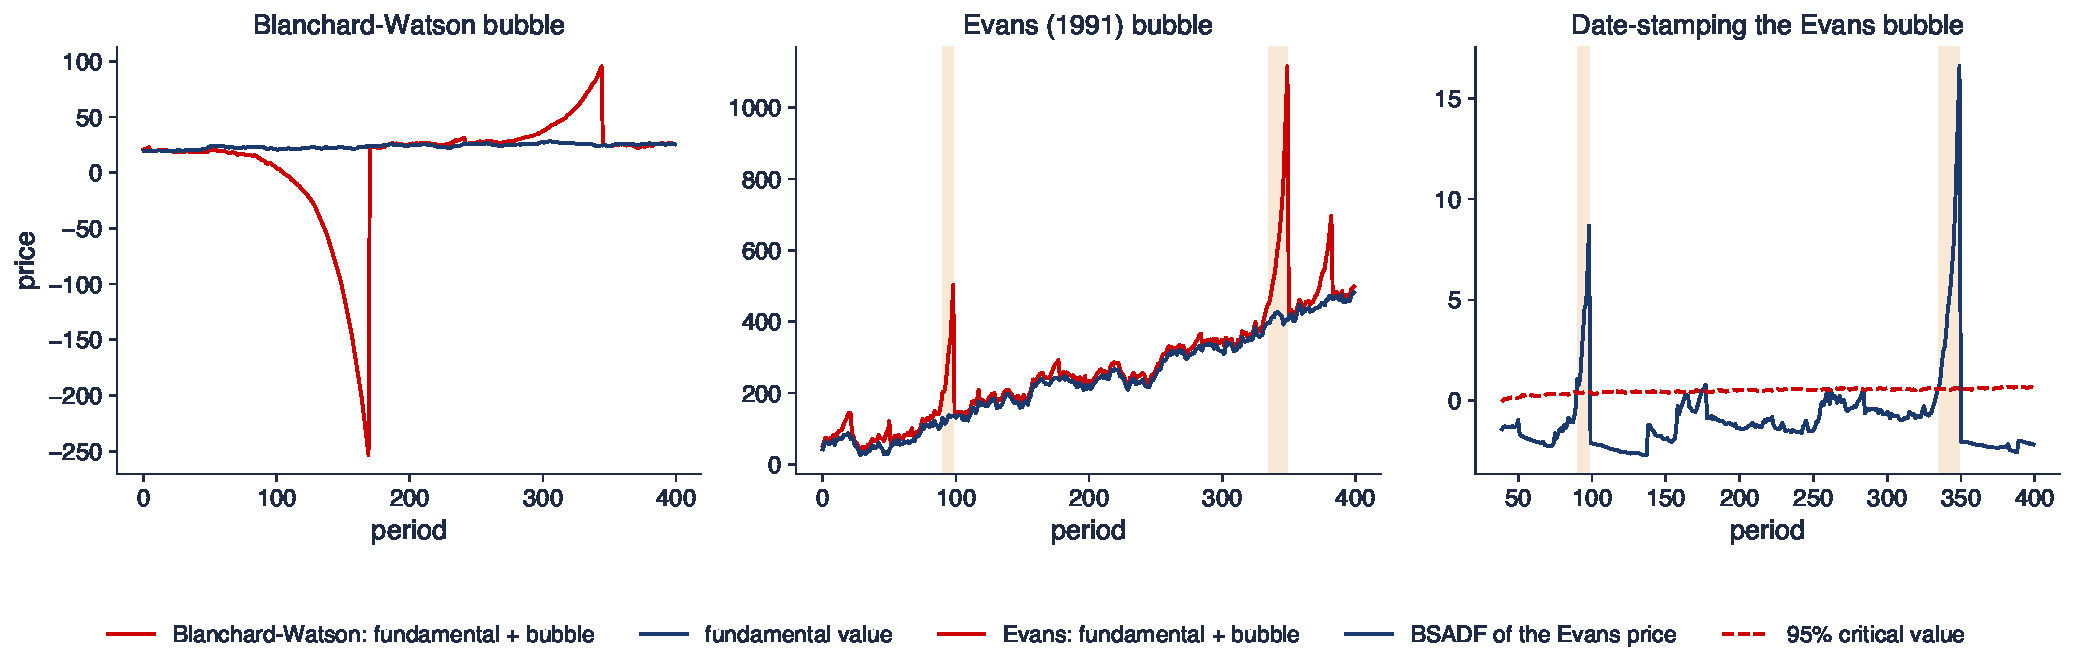
\includegraphics[width=0.97\textwidth,height=0.56\textheight,keepaspectratio]{ats_ch16_rational.pdf}
\end{center}
\vspace{-0.25cm}
\begin{itemize}
    \item Stînga: Blanchard--Watson, $r = 0{,}02$, $\pi = 0{,}98$; mijloc: bula Evans înmulțită cu 20 peste fundamentul din exemplul rezolvat ($r = 0{,}05$, $\alpha = 1$, $\delta = 0{,}5$, $\pi = 0{,}85$); dreapta: BSADF al prețului Evans față de valoarea critică punctuală de 95\% (2\,000 de traiectorii Monte Carlo)
    \item ADF pe tot eșantionul $\ensuremath{-}2{,}81$ (valoarea critică de 95\% $\ensuremath{-}0{,}07$); SADF $6{,}80$ ($1{,}45$); GSADF $16{,}58$ ($2{,}18$); 2 episoade datate
\end{itemize}
\quantlet{ATS\_ch16\_rational\_bubbles}{\qlurl{ATS_ch16_rational_bubbles}}
\end{frame}

\begin{frame}{Interpretarea bulelor simulate}
\itemsize{\small}
\begin{itemize}
    \item Traiectoria Blanchard--Watson repornește sub zero după spargere și apoi explodează în jos: exact bula negativă pe care Diba și Grossman o exclud
    \item Prețul Evans arată de cele mai multe ori ca fundamentul său; ADF pe tot eșantionul ($\ensuremath{-}2{,}81$) este chiar sub valoarea critică de 95\%: capcana lui Evans într-o singură cifră
    \item Statisticile pe ferestre văd expansiunile mari: GSADF $16{,}58$ față de $2{,}18$; șirul BSADF depășește valoarea critică doar în episoadele lungi
    \item Regula duratei minime ($6$ depășiri consecutive) păstrează 2 episoade și elimină exploziile scurte: puterea se sacrifică pentru mai puține alarme false
\end{itemize}
\end{frame}

\begin{frame}{Recapitulare: bulele raționale}
\itemsize{\small}
\begin{itemize}
    \item Prețul = fundamentul + bula, cu $\E_t B_{t+1} = (1 + r)B_t$: bula este o componentă autoregresivă explozivă
    \item Diba--Grossman: bulele nu pot fi negative și nu pot apărea ulterior; pot doar să crească sau să se spargă
    \item Evans: prăbușirile periodice ascund bula de testele pe tot eșantionul; testele recursive pe ferestre refac puterea
    \item Orice test de bulă este un test comun cu modelul fundamentului (un $r$ constant, dividende sau chirii observate)
\end{itemize}
\end{frame}


%=============================================================================
\section{Procese autoregresive explozive}
%=============================================================================

\begin{frame}{Trei regimuri ale estimatorului AR(1) (1/2)}
\itemsize{\small}
{\renewcommand{\arraystretch}{2.0}\begin{center}
\footnotesize
\begin{tabular}{@{}lll@{}}
\toprule
\textbf{Rădăcina} & \textbf{Rata și limita lui} $\hat\rho - \rho$ & \textbf{Invarianța} \\
\midrule
$|\rho| < 1$ & $\sqrt n(\hat\rho - \rho) \Rightarrow N(0, 1 - \rho^2)$ & da (CLT) \\
$\rho = 1$ & $n(\hat\rho - 1) \Rightarrow \int_0^1 W\,dW \big/ \int_0^1 W^2$ & da (FCLT) \\
$\rho = 1 + c/k_n$, $k_n \to \infty$, $k_n = o(n)$ & $\dfrac{k_n\rho_n^{\,n}}{2c}(\hat\rho - \rho_n) \Rightarrow \mathcal C$ & da \refPM{} \\
$|\rho| > 1$ fix & $\dfrac{\rho^n}{\rho^2 - 1}(\hat\rho - \rho) \Rightarrow \mathcal C$ & doar erori gaussiene \refWhi; \refAnd{} \\
\bottomrule
\end{tabular}
\end{center}
}\begin{itemize}
    \item Modelul: $y_t = \rho y_{t-1} + u_t$, $y_0 = 0$, $u_t$ i.i.d.\ $(0, \sigma^2)$; $\hat\rho$: OLS fără termen liber
    \begin{itemize}
        \item $n$: mărimea eșantionului; $W$: o mișcare browniană standard; $\mathcal C$: legea Cauchy standard; $\Rightarrow$: convergență în distribuție
        \item CLT/FCLT: teorema limită centrală (funcțională)
    \end{itemize}
\end{itemize}
\end{frame}

\begin{frame}{Trei regimuri ale estimatorului AR(1) (2/2)}
\itemsize{\small}
\begin{itemize}
    \item Rădăcină ușor explozivă: $\rho_n = 1 + c/k_n$
    \begin{itemize}
        \item $c > 0$, iar $k_n \to \infty$ mai lent decît $n$: $k_n = o(n)$, adică $k_n/n \to 0$
        \item limita Cauchy este derivată în \atsapplink{atsapp1}{atssrc1}{Anexă} % applink: limita Cauchy în cazul ușor exploziv
    \end{itemize}
    \item Rata crește de la $\sqrt n$ la $n$ și la exponențialul $\rho^n$
    \begin{itemize}
        \item cu cît sîntem mai departe de 1, cu atît învățăm mai repede $\rho$
        \item rădăcini unitare: \atschlink{https://danpele.github.io/Advanced-Time-Series/RO/Cursuri/capitol2_rupturi_structurale_modele_neliniare.pdf}{Capitolul 2} și \refHam, capitolul 17
    \end{itemize}
    \item Rădăcinile ușor explozive sînt cazul realist pentru bule
    \begin{itemize}
        \item mai rapide decît orice rădăcină locală la unitate $1 + c/n$
        \item mai lente decît orice rădăcină explozivă fixă
        \item teoria lor asimptotică nu depinde de legea erorilor, spre deosebire de cazul exploziv fix
    \end{itemize}
\end{itemize}
\end{frame}

\begin{frame}{Derivare rezolvată: de unde vine legea Cauchy}
\itemsize{\footnotesize}
\begin{itemize}
    \item $\hat\rho - \rho = \sum_{t} y_{t-1}u_t \big/ \sum_t y_{t-1}^2$ și $y_t = \sum_{j \le t}\rho^{t-j}u_j$
    \item Definim $Y_n = \sum_{j=1}^{n}\rho^{-j}u_j$ (dominat de \textbf{primele} șocuri) și $X_n = \sum_{j=1}^{n}\rho^{-(n-j)-1}u_j$ (dominat de \textbf{ultimele} șocuri)
    \begin{itemize}
        \item atunci $\rho^{-n}y_n \approx Y_n$, $\rho^{-2n}\sum_t y_{t-1}^2 \approx Y_n^2/(\rho^2 - 1)$ și $\rho^{-n}\sum_t y_{t-1}u_t \approx X_nY_n$
    \end{itemize}
    \item Deci $\dfrac{\rho^n}{\rho^2 - 1}(\hat\rho - \rho) \approx \dfrac{X_n}{Y_n}$
    \begin{itemize}
        \item $X_n$ și $Y_n$ folosesc asimptotic blocuri disjuncte de șocuri: independente, cu dispersii egale $\sigma^2/(\rho^2 - 1)$
        \item $\rho$ \textbf{fix}: fiecare sumă este dominată de cîteva șocuri; este gaussiană doar dacă $u_j$ sînt gaussiene, deci raportul este Cauchy doar atunci \refAnd
        \item $\rho_n$ \textbf{ușor exploziv}: aproximativ $k_n \to \infty$ șocuri intră în fiecare sumă cu ponderi comparabile, se aplică o teoremă limită centrală, iar $X_n/Y_n \Rightarrow \mathcal C$ pentru orice erori i.i.d.\ cu dispersie finită \refPM
    \end{itemize}
    \item Inferență pivotală: intervalul de 95\% $\hat\rho \pm (\hat\rho^2 - 1)\hat\rho^{-n}\tan(0{,}475\pi)$, cu $\tan(0{,}475\pi) \approx 12{,}71$, înlocuiește $\rho$ cu $\hat\rho$ în factorul de normare
\end{itemize}
\end{frame}

\begin{frame}{Limitele Cauchy în eșantioane finite}
\itemsize{\footnotesize}
\begin{center}
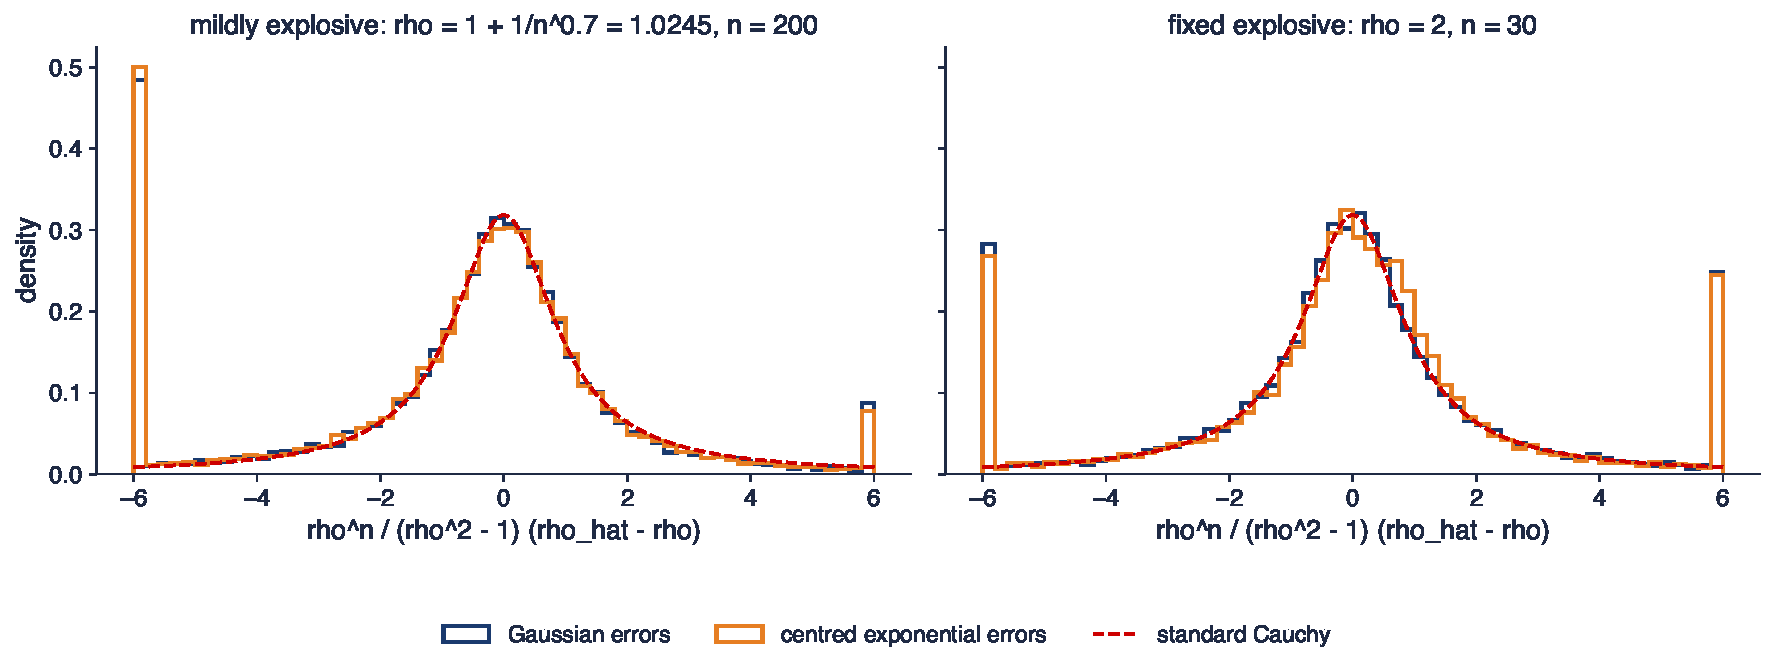
\includegraphics[width=0.97\textwidth,height=0.55\textheight,keepaspectratio]{ats_ch16_asymptotics.pdf}
\end{center}
\vspace{-0.25cm}
\begin{itemize}
    \item 20\,000 de eșantioane; eroarea normată $\rho^n(\hat\rho - \rho)/(\rho^2 - 1)$ cu erori gaussiene și exponențiale centrate (asimetrice), față de densitatea Cauchy
    \item Distanța Kolmogorov--Smirnov față de Cauchy: ușor exploziv, $n = 200$: 0{,}060 și 0{,}062; $n = 2000$ ($\rho = 1{,}0049$): 0{,}011 ($p$ = 0{,}620) și 0{,}007 ($p$ = 0{,}945); $\rho = 2$ fix: 0{,}007 ($p$ = 0{,}263) și 0{,}025 ($p$ $<$ 0{,}001)
\end{itemize}
\quantlet{ATS\_ch16\_explosive\_asymptotics}{\qlurl{ATS_ch16_explosive_asymptotics}}
\end{frame}

\begin{frame}{Interpretarea limitelor Cauchy}
\itemsize{\small}
\begin{itemize}
    \item Rădăcină fixă: cu erori gaussiene legea Cauchy se potrivește ($p$ = 0{,}263); cu erori asimetrice este respinsă ($p$ $<$ 0{,}001): nu există un principiu de invarianță, cum a arătat Anderson
    \item Rădăcină ușor explozivă: la $n = 2000$ ambele legi ale erorilor dau legea Cauchy; la $n = 200$ ($k_n = 40{,}8$) aproximarea este încă grosieră pentru ambele: teorema limită centrală din $X_n$ și $Y_n$ cere multe șocuri efective
    \item Acoperirea intervalului Cauchy de 95\%: 97{,}0\% și 97{,}2\% ($n = 200$), 95{,}0\% și 94{,}7\% ($n = 2000$): conservator în eșantioane mici, precis în eșantioane mari
    \item Pentru testele de bulă aceasta este o veste bună: alternativa explozivă se învață cu rată exponențială, deci statisticile pe ferestre diverg repede cînd o fereastră se află în interiorul bulei
\end{itemize}
\end{frame}

\begin{frame}{De la teoria asimptotică la testele de bulă}
\itemsize{\small}
\begin{itemize}
    \item Sub o alternativă ușor explozivă statistica $t$ ADF diverge la $+\infty$: testele pe coada din dreapta sînt \textbf{consistente} \refPSYb
    \item Niveluri față de logaritmi: o bulă rațională este explozivă în \textbf{nivel}; în logaritmi, o traiectorie pură $\ln B_0 + t\ln(1 + r)$ este o tendință liniară
    \begin{itemize}
        \item $\ln(F_t + B_t)$ \textbf{accelerează} cît timp ponderea bulei crește: testele pe logaritmul prețului vizează accelerarea, ceea ce testează în practică PWY și PSY
    \end{itemize}
    \item Specificația contează: termenul liber, o derivă slabă $dT^{-\eta}$ ($\eta > 1/2$) sub ipoteza nulă și numărul de laguri schimbă limita sub ipoteza nulă și nivelul testului \refPSYs
    \item Prăbușirile: o scădere bruscă este o fază ușor \textbf{integrată} sau staționară după cea explozivă; \refPSi{} datează implozia cu o regresie inversă
\end{itemize}
\end{frame}

\begin{frame}{Recapitulare: procesele autoregresive explozive}
\itemsize{\small}
\begin{itemize}
    \item Rădăcinile explozive se învață cu rata $\rho^n$; limita este Cauchy, un raport de două normale independente construite din primele și ultimele șocuri
    \item Rădăcinile explozive fixe nu au un principiu de invarianță; cele ușor explozive au, de aceea sînt modelul de lucru pentru bule
    \item Intervalul Cauchy pentru $\rho$ este pivotal, dar cere eșantioane mari; testele pe coada din dreapta sînt consistente față de alternative ușor explozive
\end{itemize}
\end{frame}


%=============================================================================
\section{Testele recursive: teorie și nivel}
%=============================================================================

\begin{frame}{Statisticile recursive (1/2)}
\itemsize{\small}
\begin{itemize}
    \item \textbf{Regresia pe fereastră} pentru logaritmul prețului $y_t$, pe fracțiunile de eșantion $[r_1, r_2]$ \[ \Delta y_t = a + \delta y_{t-1} + \sum_{j=1}^{k}\phi_j\Delta y_{t-j} + e_t, \qquad t = \lfloor r_1T\rfloor, \dots, \lfloor r_2T\rfloor \]
    \begin{itemize}
        \item $\Delta y_t = y_t - y_{t-1}$; $a$: termenul liber; $\delta$: coeficientul testat; $\phi_j$: coeficienții celor $k$ diferențe cu lag; $e_t$: eroarea; $T$: mărimea eșantionului; $\lfloor\cdot\rfloor$: partea întreagă
        \item $\mathrm{ADF}_{r_1}^{r_2}$: statistica $t$ a lui $\delta$ pe această fereastră
    \end{itemize}
    \item $H_0$: $\delta = 0$ (rădăcină unitară) față de $H_1$: $\delta > 0$ (explozivă): un test pe \textbf{coada din dreapta}
    \begin{itemize}
        \item fracțiunea minimă a ferestrei $r_0 = 0{,}01 + 1{,}8/\sqrt T$
    \end{itemize}
    \item \textbf{Supremele} pe ferestre \refPWY, \refPSYa{} \[ \mathrm{SADF} = \sup_{r_2 \in [r_0, 1]}\mathrm{ADF}_0^{r_2}, \quad \mathrm{BSADF}_{r_2} = \sup_{r_1 \in [0, r_2 - r_0]}\mathrm{ADF}_{r_1}^{r_2}, \quad \mathrm{GSADF} = \sup_{r_2}\mathrm{BSADF}_{r_2} \]
    \begin{itemize}
        \item SADF: ferestre care încep cu prima observație; BSADF: toate ferestrele care se termină în $r_2$ (folosit la datare); GSADF: toate ferestrele
    \end{itemize}
\end{itemize}
\end{frame}

\begin{frame}{Statisticile recursive (2/2)}
\itemsize{\small}
\begin{itemize}
    \item Limita sub ipoteza nulă (PSY, teorema 1), cu $r_w = r_2 - r_1$ și integrale pe $[r_1, r_2]$: \[ \mathrm{ADF}_{r_1}^{r_2} \Rightarrow \dfrac{\frac12 r_w\left[W(r_2)^2 - W(r_1)^2 - r_w\right] - \int W\,dr\,\left[W(r_2) - W(r_1)\right]}{r_w^{1/2}\left\{r_w\int W^2dr - \left(\int W\,dr\right)^2\right\}^{1/2}} \]
    \begin{itemize}
        \item $W$: o mișcare browniană standard; $\Rightarrow$: convergență în distribuție cînd $T \to \infty$
        \item pivotală: nu depinde de $\sigma$ și de derivă, deci valorile critice depind doar de $r_0$, de termenii determiniști și, în eșantioane finite, de $T$
    \end{itemize}
    \item Calcul: pentru $T = 400$ există 65\,341 de regresii pe ferestre; produsele încrucișate cumulate le dau pe toate în $O(T^2)$ operații
\end{itemize}
\end{frame}

\begin{frame}{Distribuțiile sub ipoteza nulă și valorile critice}
\itemsize{\footnotesize}
\begin{center}
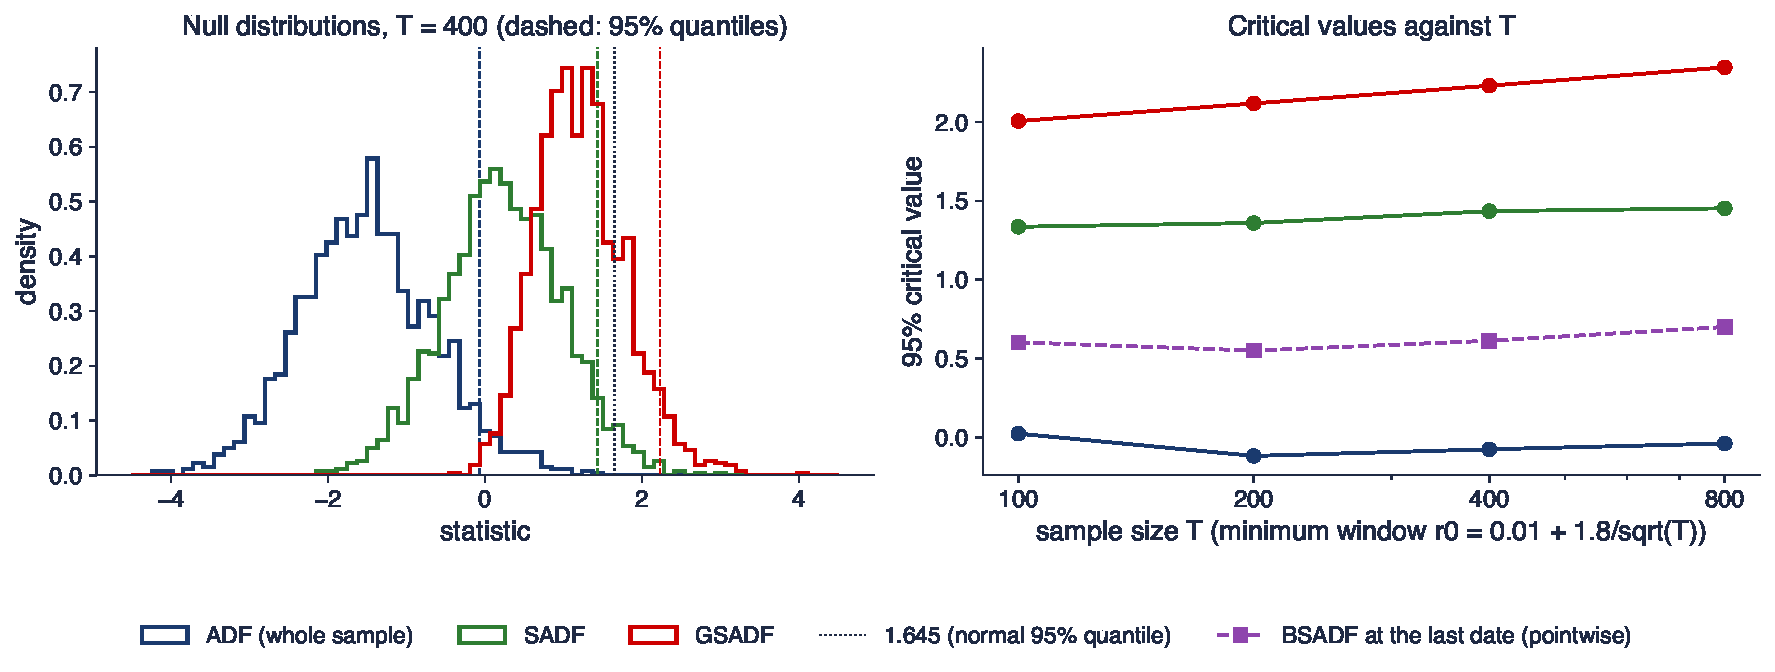
\includegraphics[width=0.97\textwidth,height=0.65\textheight,keepaspectratio]{ats_ch16_null.pdf}
\end{center}
\vspace{-0.25cm}
\begin{itemize}
    \item Modelul nul $y_t = T^{-1} + y_{t-1} + e_t$, $e_t \sim N(0, 1)$, fără laguri; valori critice de 95\% la $T = 100, 200, 400, 800$: SADF 1{,}34; 1{,}36; 1{,}43; 1{,}45; GSADF 2{,}01; 2{,}12; 2{,}23; 2{,}35
\end{itemize}
\quantlet{ATS\_ch16\_recursive\_tests}{\qlurl{ATS_ch16_recursive_tests}}
\end{frame}

\begin{frame}{Interpretarea distribuțiilor sub ipoteza nulă}
\itemsize{\small}
\begin{itemize}
    \item ADF pe tot eșantionul are cuantila de 95\% negativă (\ensuremath{-}0{,}07 la $T = 400$): folosind 1,645 nu s-ar respinge aproape niciodată, coada dreaptă a legii Dickey--Fuller este scurtă
    \item Fiecare suprem mută distribuția spre dreapta: SADF caută pe punctele de sfîrșit, GSADF pe punctele de început și de sfîrșit; pragul GSADF este prețul căutării
    \item Valoarea critică GSADF crește cu $T$ (de la 2{,}01 la 2{,}35) deși $r_0$ scade: mai multe ferestre, un maxim mai mare; simulați valorile critice pentru propriile $T$, $r_0$ și număr de laguri
    \item Cuantila punctuală de 95\% a BSADF la ultima dată (0{,}61 la $T = 400$) este mult sub cea GSADF: o singură dată este testată la 5\%, întreaga traiectorie nu
\end{itemize}
\end{frame}

\begin{frame}{Volatilitate variabilă și wild bootstrap}
\itemsize{\small}
\begin{itemize}
    \item Limita pivotală presupune șocuri homoscedastice; cu o schimbare a volatilității limita depinde de profilul dispersiei, iar valorile critice Monte Carlo dau un nivel greșit \refHLST
    \begin{itemize}
        \item o creștere tîrzie a volatilității arată ca o accelerare; o scădere a volatilității face testul conservator
    \end{itemize}
    \item \textbf{Wild bootstrap} \refPS: estimăm modelul nul $\Delta y_t = \mu + \sum_j\phi_j\Delta y_{t-j} + e_t$, extragem semne Rademacher $w_t = \pm 1$, construim $\Delta y^*_t = \sum_j\hat\phi_j\Delta y^*_{t-j} + w_t\hat e_t$, cumulăm și recalculăm statisticile
    \begin{itemize}
        \item seria bootstrap are prin construcție o rădăcină unitară și \textbf{același tipar al volatilității} $|\hat e_t|$ ca datele
        \item valori critice: cuantilele punctuale ale BSADF, cuantila maximului (GSADF) sau cuantila maximului pe o fereastră mobilă
    \end{itemize}
    \item Alternative pentru volatilitatea nestaționară: statistici ponderate și statistici pe baza semnelor \refHLZ; teste pentru finalul eșantionului \refAHLT
\end{itemize}
\end{frame}

\begin{frame}{Multe date, o alarmă falsă}
\itemsize{\small}
\begin{itemize}
    \item Datarea compară $\mathrm{BSADF}_{r_2}$ cu o valoare critică \textbf{punctuală} la fiecare dată: fiecare dată are o probabilitate de 5\% de alarmă falsă, dar un eșantion are sute de date
    \begin{itemize}
        \item BSADF este puternic autocorelat în $r_2$, deci alarmele false vin în serii: regula duratei minime elimină doar seriile cele mai scurte
    \end{itemize}
    \item \textbf{Rata erorii de familie} (FWER): probabilitatea a cel puțin unei alarme false pe o mulțime de date
    \begin{itemize}
        \item pe tot eșantionul: comparăm BSADF cu cuantila de 95\% a maximului său, adică valoarea critică GSADF
        \item pe o fereastră mobilă de $\tau_b$ date \refPS: cuantila bootstrap de 95\% a lui $\max_{s \in (t - \tau_b, t]}\mathrm{BSADF}_s$; aici $\tau_b = 52$ de săptămîni
    \end{itemize}
    \item Asimptotic, datarea consistentă cere valori critice care diverg încet, astfel încît probabilitatea alarmei false să dispară \refPSYb; în practică se folosește un 5\% fix la fiecare dată, iar costul lui trebuie măsurat
\end{itemize}
\end{frame}

\begin{frame}{Nivelul testelor sub volatilitate variabilă și pe multe date}
\itemsize{\footnotesize}
\begin{center}
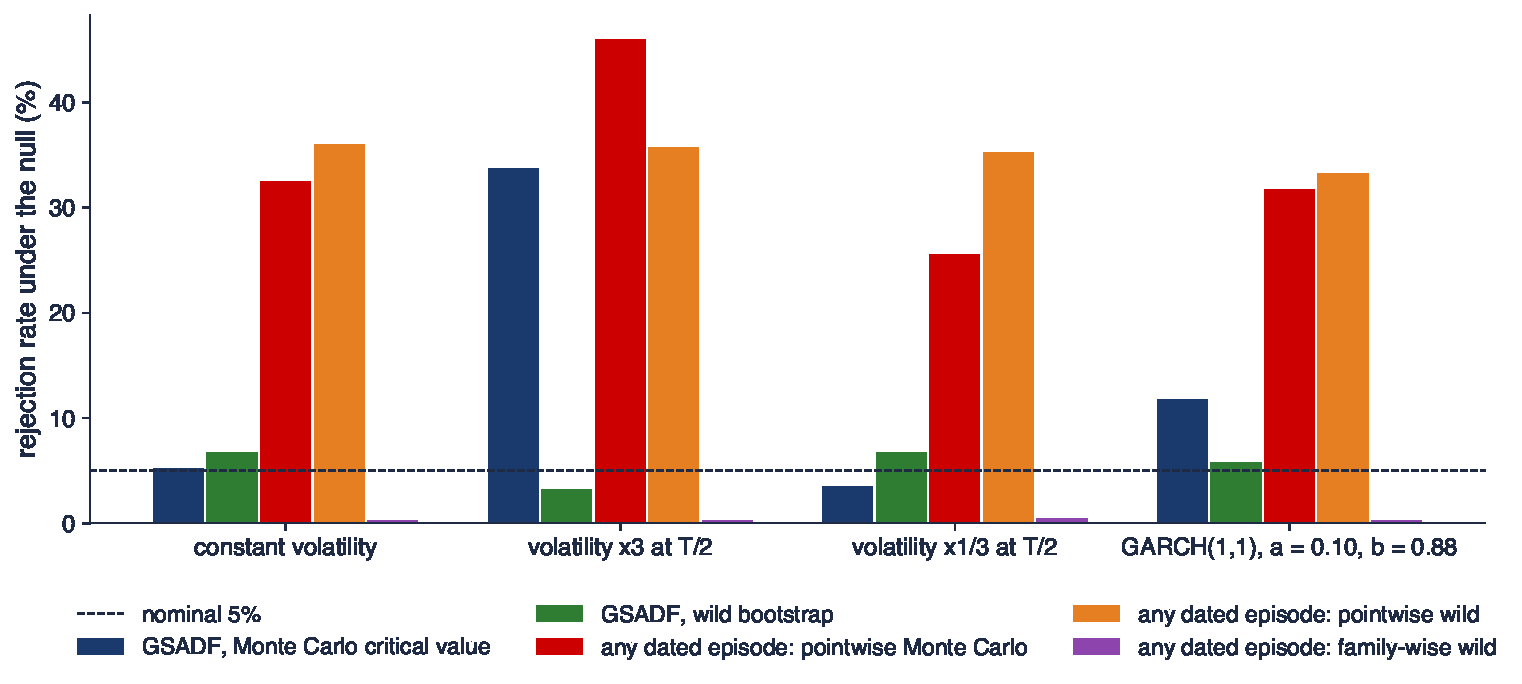
\includegraphics[width=0.97\textwidth,height=0.65\textheight,keepaspectratio]{ats_ch16_size.pdf}
\end{center}
\vspace{-0.25cm}
\begin{itemize}
    \item 400 de traiectorii sub ipoteza nulă cu $T = 200$ pentru fiecare design, fiecare cu propriul wild bootstrap (199 de extrageri); un episod datat cere 6 depășiri consecutive; nivelul nominal 5\%
\end{itemize}
\quantlet{ATS\_ch16\_size\_wild\_bootstrap}{\qlurl{ATS_ch16_size_wild_bootstrap}}
\end{frame}

\begin{frame}{Interpretarea studiului de nivel}
\itemsize{\small}
\begin{itemize}
    \item GSADF cu valori critice Monte Carlo: 5{,}2\% cu volatilitate constantă, 33{,}8\% după o triplare tîrzie, 11{,}8\% sub GARCH; wild bootstrap dă 6{,}8\%, 3{,}2\% și 5{,}8\%
    \item Datarea punctuală găsește cel puțin un episod în 32{,}5\% (Monte Carlo) și 36{,}0\% (wild) dintre traiectoriile \textbf{fără nicio bulă}, chiar cu volatilitate constantă
    \item Cu pragul de familie pe tot eșantionul, episoadele false scad la 0{,}2\%--0{,}5\%: sub 5\%, fiindcă un episod cere și 6 depășiri consecutive; costul este puterea și datări mai tîrzii
    \item Concluzia: raportați ce rată de eroare controlează un episod datat; un test punctual de 5\% în fiecare săptămînă nu este un test de 5\% pentru eșantion
\end{itemize}
\end{frame}

\begin{frame}{Recapitulare: testele recursive}
\itemsize{\small}
\begin{itemize}
    \item SADF, GSADF și BSADF sînt supreme ale statisticilor ADF pe ferestre, cu o limită pivotală sub ipoteza nulă; valorile critice trebuie să corespundă lui $T$, $r_0$, termenilor determiniști și lagurilor
    \item Volatilitatea variabilă distorsionează nivelul; wild bootstrap păstrează tiparul volatilității și îl reface
    \item Datarea punctuală are o rată mare de episoade false pe un eșantion; pragurile de familie o controlează, cu prețul puterii
\end{itemize}
\end{frame}


%=============================================================================
\section{Datarea și avertizarea timpurie}
%=============================================================================

\begin{frame}{Regulile de datare și acuratețea lor}
\itemsize{\small}
\begin{itemize}
    \item \textbf{Începutul și sfîrșitul} \refPSYa: prima dată la care BSADF depășește valoarea critică și prima dată ulterioară la care coboară sub ea \[ \hat r_e = \inf\{r_2 \ge r_0: \mathrm{BSADF}_{r_2} > cv_{r_2}\}, \qquad \hat r_f = \inf\{r_2 \ge \hat r_e + \delta\ln(T)/T: \mathrm{BSADF}_{r_2} < cv_{r_2}\} \]
    \begin{itemize}
        \item $cv_{r_2}$: valoarea critică punctuală de 95\% la $r_2$; $\delta\ln(T)/T$: o durată minimă (cu $\delta$ o constantă de calibrare)
        \item aici: un episod este o serie de cel puțin $\lceil\ln T\rceil$ depășiri consecutive, datată de la prima la ultima (ca în \texttt{exuber} \refVPM)
    \end{itemize}
    \item În timp real, un episod este \textbf{confirmat} doar după durata minimă: data alarmei este începutul plus $\lceil\ln T\rceil - 1$
    \item Consistența lui $(\hat r_e, \hat r_f)$ este valabilă pentru bule ușor explozive cu durată fracționară fixă \refPSYb
    \begin{itemize}
        \item începutul este datat tîrziu, fiindcă o fereastră trebuie să acumuleze întîi observații explozive
        \item estimatori îmbunătățiți ai începutului și sfîrșitului, care folosesc toată perioada bulei: \refHLS
    \end{itemize}
\end{itemize}
\end{frame}

\begin{frame}{Datarea: designul experimentului}
\itemsize{\small}
\begin{itemize}
    \item Traiectorii simulate: mers aleator de la $y_0 = 100$, apoi o fază explozivă, o prăbușire și din nou mers aleator
    \begin{itemize}
        \item faza explozivă $y_t = \rho y_{t-1} + e_t$, $\rho > 1$, în perioadele 200--260; $e_t$: zgomot cu distribuția Normală
        \item prăbușire la nivelul de dinaintea bulei la sfîrșitul fazei explozive
        \item $T = 400$, 1\,000 de traiectorii pentru fiecare valoare a lui $\rho$
    \end{itemize}
    \item Întrebările: cît de des este găsită bula, cît de tîrziu este datat începutul ei, cît de des este datat un episod fals înaintea ei?
\end{itemize}
\end{frame}

\begin{frame}{Cît de tîrziu este datat începutul?}
\itemsize{\footnotesize}
\begin{center}
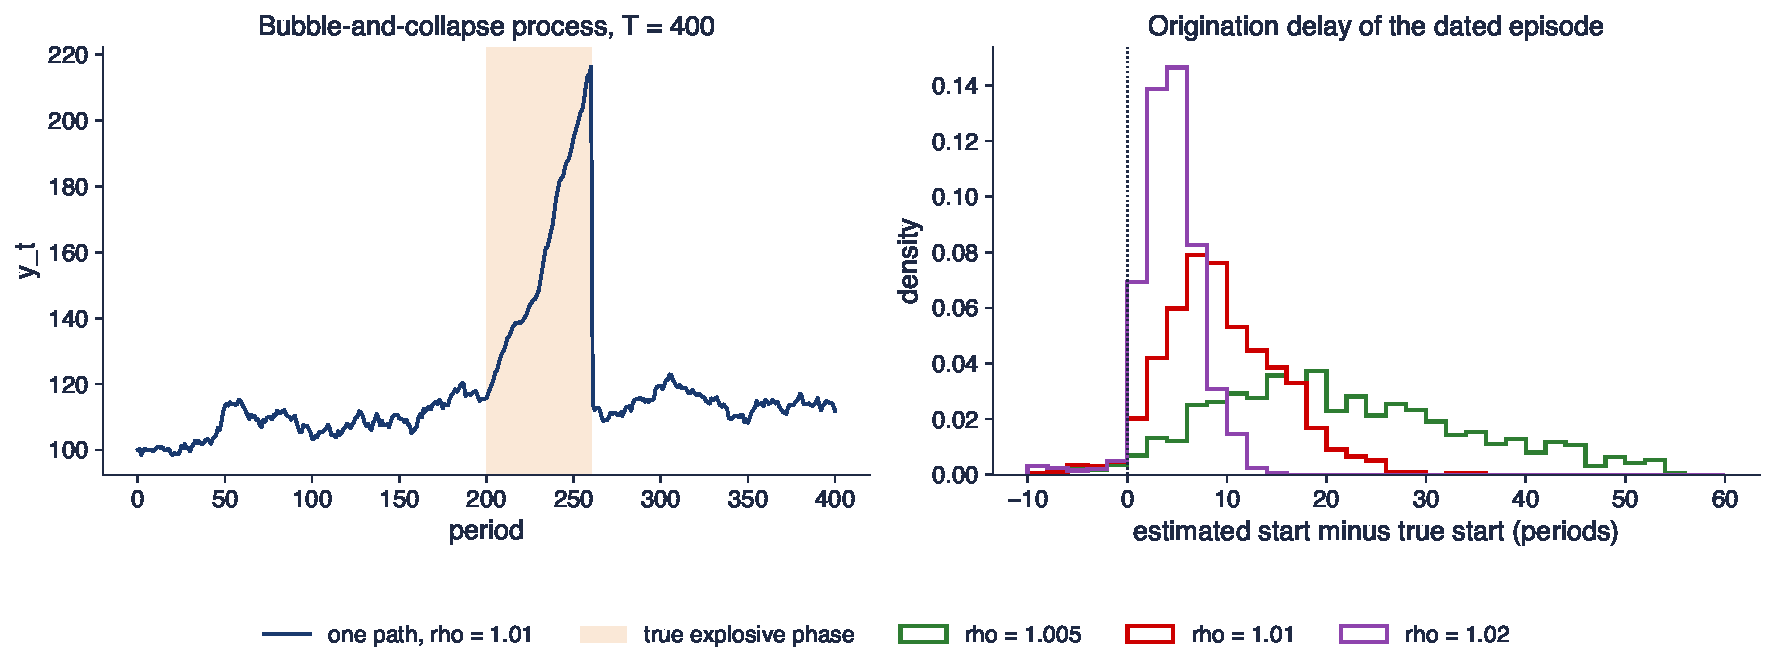
\includegraphics[width=0.97\textwidth,height=0.65\textheight,keepaspectratio]{ats_ch16_dating.pdf}
\end{center}
\vspace{-0.25cm}
\begin{itemize}
    \item Întîrzierea primei depășiri datate după începutul adevărat (perioade); valori critice punctuale de 95\% Monte Carlo; creșterea pe durata bulei $\rho^{60}$: 1{,}35; 1{,}82 și 3{,}28
\end{itemize}
\quantlet{ATS\_ch16\_date\_stamping}{\qlurl{ATS_ch16_date_stamping}}
\end{frame}

\begin{frame}{Interpretarea experimentului de datare}
\itemsize{\small}
\begin{itemize}
    \item Ratele de detecție 94{,}9\%, 100{,}0\% și 100{,}0\% pentru $\rho = 1{,}005, 1{,}01, 1{,}02$: o bulă de 60 de perioade este găsită aproape întotdeauna
    \item Întîrzieri mediane ale începutului 19, 8 și 4 perioade (intervale intercuartilice 11--29, 5--13, 2--6); confirmarea adaugă 6 $-$ 1 perioade: mediane 24, 13, 9
    \item Pentru bula cea mai lentă, alarma vine după aproximativ o treime din viața ei: un detector al exuberanței \textbf{în desfășurare}, nu al nașterii ei
    \item În 26\%--31\% dintre traiectorii este datat un episod fals \textbf{înainte} de începutul bulei: multiplicitatea din secțiunea anterioară, acum într-un design cu bulă reală
\end{itemize}
\end{frame}

\begin{frame}{Monitorizarea în timp real (1/2)}
\itemsize{\small}
\begin{itemize}
    \item Monitorizarea: un eșantion de antrenare de $n$ observații fără bulă, apoi o decizie la fiecare dată nouă $t > n$; rata de eroare se referă la \textbf{întregul} orizont de monitorizare \refCSW
    \item \textbf{CUSUM} al randamentelor: abaterile cumulate ale randamentelor noi de la media din perioada de antrenare, în unități ale volatilității din antrenare \[ S_t = \sum_{j=n+1}^{t}\frac{r_j - \bar r_n}{\hat\sigma_n\sqrt n}, \qquad \text{alarmă cînd}\ S_t > b_t = \sqrt{\tfrac{t - n}{n}\cdot\tfrac{t}{n}\left[a^2 + \ln\tfrac{t}{t - n}\right]} \]
    \begin{itemize}
        \item $r_j$: randamentul perioadei $j$; $\bar r_n$, $\hat\sigma_n$: media și abaterea standard a randamentelor din antrenare; $b_t$: frontiera, care se lărgește cu $t$; $a$: o constantă care fixează rata de eroare
    \end{itemize}
    \item Rata de eroare pe întregul orizont (demonstrația în \atsapplink{atsapp2}{atssrc2}{Anexă})
    \begin{itemize}
        \item $\Pr\{S_t > b_t$ pentru un $t\} \to 1 - \Phi(a) + a\varphi(a)$; $\Phi$, $\varphi$: funcția de repartiție și densitatea distribuției Normale standard
        \item 5\% dă $a = 2{,}50$, $a^2 = 6{,}25$
    \end{itemize}
\end{itemize}
\end{frame}

\begin{frame}{Monitorizarea în timp real (2/2)}
\itemsize{\small}
\begin{itemize}
    \item Nivelul simulat, $n = 100$, orizont $5n$, 2\,000 de traiectorii
    \begin{itemize}
        \item 3{,}5\% cu randamente i.i.d., 6{,}0\% cu randamente GARCH
    \end{itemize}
    \item \refHB{} compară testele de bulă și schemele de monitorizare și recomandă în timp real monitorizarea de acest tip
    \begin{itemize}
        \item \refAHLST{} propun statistici de monitorizare cu nivel controlat pentru bule explozive
    \end{itemize}
    \item BSADF în timp real este și el un monitor: $\mathrm{BSADF}_t$ folosește doar datele pînă la $t$, dar valorile lui critice punctuale nu controlează eroarea pe orizont
\end{itemize}
\end{frame}

\begin{frame}{Monitorizarea Nasdaq 100 și Bitcoin}
\itemsize{\footnotesize}
\begin{center}
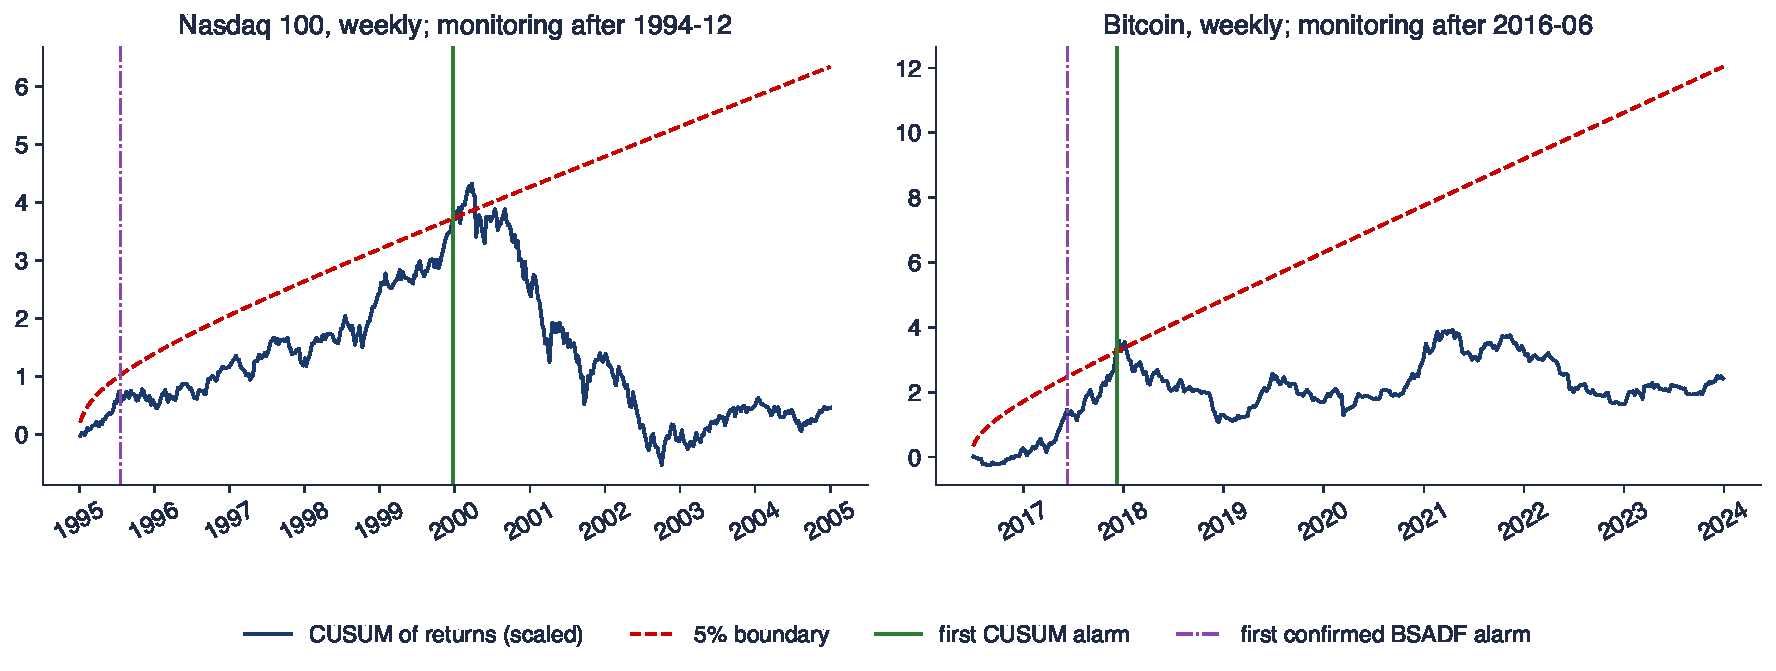
\includegraphics[width=0.97\textwidth,height=0.65\textheight,keepaspectratio]{ats_ch16_monitor.pdf}
\end{center}
\vspace{-0.25cm}
\begin{itemize}
    \item Randamente logaritmice săptămînale; antrenare: 1990--1994 (Nasdaq 100, $n = 260$) și septembrie 2014 -- iunie 2016 (Bitcoin, $n = 92$); BSADF cu valori critice punctuale Monte Carlo
\end{itemize}
\quantlet{ATS\_ch16\_monitoring}{\qlurl{ATS_ch16_monitoring}}
\end{frame}

\begin{frame}{Interpretarea graficelor de monitorizare}
\itemsize{\small}
\begin{itemize}
    \item Nasdaq 100: alarma CUSUM apare pe 24 decembrie 1999, cu trei luni înaintea maximului din 24 martie 2000; prima alarmă BSADF confirmată după antrenare apare pe 21 iulie 1995, cu peste patru ani mai devreme
    \item Bitcoin: CUSUM pe 8 decembrie 2017, la vîrful creșterii din 2017; BSADF pe 9 iunie 2017
    \begin{itemize}
        \item frontiera se lărgește ca $\sqrt{t\ln t}$, deci după 2018 creșterea din 2021 nu o mai poate atinge
    \end{itemize}
    \item CUSUM detectează o schimbare a randamentului mediu (o accelerare persistentă), nu explozivitatea ca atare; este lent, dar nivelul lui este controlat pe tot orizontul
    \item BSADF reacționează devreme și des: o alarmă timpurie urmată de ani de creșteri suplimentare este costisitoare pentru oricine acționează pe baza ei
\end{itemize}
\end{frame}

\begin{frame}{Evaluarea onestă a avertizărilor timpurii}
\itemsize{\small}
\begin{itemize}
    \item Definiți \textbf{evenimentul} înainte de a vă uita la alarme: aici o scădere de cel puțin 20\% în următoarele 182 de zile; definiți regula de \textbf{alarmă} și datele de evaluare (fiecare a cincea zi de tranzacționare)
    \item Rata de detecție $H = \Pr(\text{alarmă} \mid \text{eveniment})$, rata alarmelor false $F = \Pr(\text{alarmă} \mid \text{fără eveniment})$, frecvența de bază $\pi_0 = \Pr(\text{eveniment})$
    \begin{itemize}
        \item \textbf{precizia} din regula lui Bayes: $\Pr(\text{eveniment} \mid \text{alarmă}) = H\pi_0 / [H\pi_0 + F(1 - \pi_0)]$; cu $\pi_0 = 5\%$, $H = 80\%$, $F = 20\%$ este doar 17\%
        \item raportul zgomot/semnal $F/H$ din literatura avertizărilor timpurii \refKLR
    \end{itemize}
    \item \textbf{Curba ROC}: $(F, H)$ pentru fiecare prag al unui scor continuu; \textbf{AUC} $= \Pr(\text{scorul unei date cu eveniment} > \text{scorul unei date fără eveniment})$; 0,5 înseamnă lipsa abilității
    \item Orizonturile suprapuse fac datele de evaluare puternic dependente: intervalele pentru AUC cer un moving-block bootstrap (\atschlink{https://danpele.github.io/Advanced-Time-Series/RO/Cursuri/capitol0_recapitulare_inferenta.pdf}{Capitolul 0}), iar cîteva crahuri poartă tot eșantionul
\end{itemize}
\end{frame}

\begin{frame}{Recapitulare: datarea și avertizarea timpurie}
\itemsize{\small}
\begin{itemize}
    \item BSADF datează începutul tîrziu (după o serie de observații explozive) și îl confirmă și mai tîrziu; bulele lente sînt găsite după o parte mare din viața lor
    \item Monitorizarea cu o frontieră controlează eroarea pe tot orizontul; BSADF punctual nu o face
    \item Evaluați alarmele prin rata de detecție, rata alarmelor false, precizia la frecvența de bază și ROC/AUC, cu intervale prin block bootstrap
\end{itemize}
\end{frame}


%=============================================================================
\section{Fundamentele față de prețuri}
%=============================================================================

\begin{frame}{Testarea raportului, a prețului și a fundamentului}
\itemsize{\footnotesize}
\begin{columns}[T]
\begin{column}{0.34\textwidth}
\centering
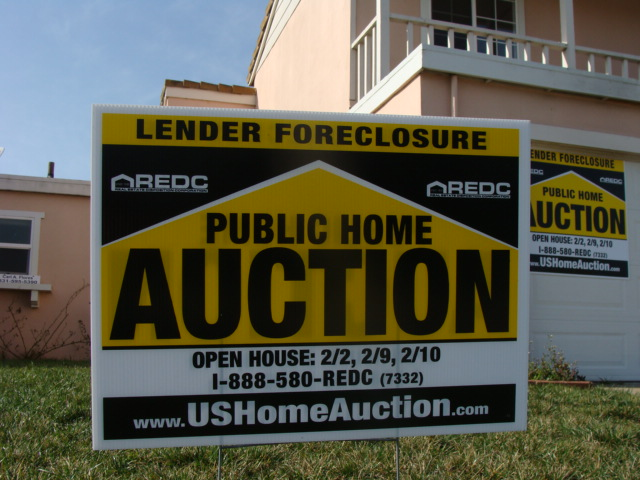
\includegraphics[height=0.36\textheight]{ch16_foreclosure_2008.jpg}\\[1mm]
\imgcap{O locuință executată silit în SUA, 2008}
\imgcredit{https://commons.wikimedia.org/wiki/File:Foreclosedhome.JPG}{Foto: Brendel (2008); CC BY-SA 3.0; Wikimedia Commons}
\end{column}
\begin{column}{0.64\textwidth}
\begin{itemize}
    \item În modelul valorii actualizate, raportul preț/chirie (sau preț/dividend) este staționar; un \textbf{raport} exploziv cu un \textbf{fundament} neexploziv indică o bulă
    \item Dacă chiriile explodează ele însele, un preț exploziv nu dovedește o bulă: testați ambele (logica din \refDGb{} aplicată cu PSY)
    \item Lucrări de referință: \refPY{} datează exuberanța raportului preț/chirie din SUA dinaintea crizei subprime; \refPav{} aplică GSADF pe baza de date internațională a prețurilor locuințelor a Fed din Dallas
    \item Prețurile lunare ale locuințelor sînt netezite (indici de vînzări repetate, evaluări): variațiile lor sînt autocorelate, deci numărul de laguri $k$ contează; aici $k$ după BIC, pînă la 6 luni
\end{itemize}
\end{column}
\end{columns}
\end{frame}

\begin{frame}{Locuințele din SUA și din România: raportul și fundamentul}
\itemsize{\footnotesize}
\begin{center}
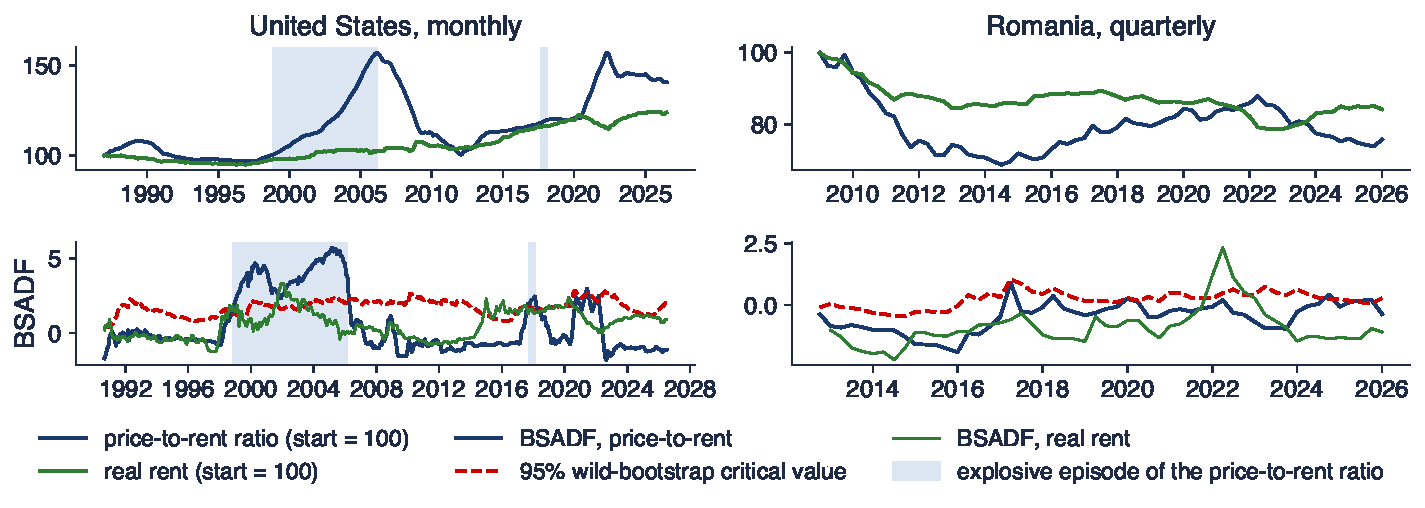
\includegraphics[width=0.97\textwidth,height=0.65\textheight,keepaspectratio]{ats_ch16_housing.pdf}
\end{center}
\vspace{-0.25cm}
\begin{itemize}
    \item Logaritmul raportului preț/chirie și al chiriei reale; BSADF cu $k$ laguri (raportul SUA $k = 1$, chiria $k = 1$) și valori critice punctuale de 95\% prin wild bootstrap (999 de extrageri); zonele colorate: episoadele datate ale raportului
\end{itemize}
\quantlet{ATS\_ch16\_housing}{\qlurl{ATS_ch16_housing}}
\end{frame}

\begin{frame}{Interpretarea testelor pe locuințe}
\itemsize{\footnotesize}
\begin{itemize}
    \item Raportul preț/chirie din SUA: GSADF 5{,}75 față de valoarea wild bootstrap 4{,}47; episodul principal durează din noiembrie 1998 pînă în martie 2006, boom-ul dinaintea crizei subprime găsit de \refPY
    \item Chiria reală în SUA: GSADF 3{,}35 față de 3{,}25, cu episoadele februarie 1998--martie 1999; iunie 2001--septembrie 2004; septembrie 2014--mai 2021; septembrie 2023--aprilie 2026: și fundamentul a accelerat, deci creșterea prețurilor din 2014--2022 ține parțial de chirii
    \item Prețul real al locuințelor din SUA, singur: episoadele februarie 2002--martie 2006; decembrie 2020--mai 2022; creșterea din 2020--2022 este explozivă în preț, dar nu în raport, spre deosebire de 1998--2006
    \item România (trimestrial, $T = 68$): GSADF al raportului 0{,}91 față de 1{,}38, al prețului real 0{,}88 față de 2{,}11: niciun episod exploziv din 2009; indicele HICP al chiriilor crește cu 33\% în aprilie 2026, de aceea eșantionul se încheie în martie 2026
\end{itemize}
\end{frame}

\begin{frame}{Recapitulare: fundamentele față de prețuri}
\itemsize{\small}
\begin{itemize}
    \item Testați separat raportul și fundamentul: un raport exploziv cu un fundament liniștit este semnătura bulei
    \item Indicii neteziți ai locuințelor cer laguri în regresie și un bootstrap sub ipoteza nulă AR; fără laguri testele resping aproape peste tot
    \item Eșantioanele scurte (România din 2009) au putere mică: lipsa respingerii nu dovedește lipsa bulei
\end{itemize}
\end{frame}


%=============================================================================
\section{LPPLS ca detector alternativ}
%=============================================================================

\begin{frame}{LPPLS într-un singur slide}
\itemsize{\footnotesize}
\begin{columns}[T]
\begin{column}{0.3\textwidth}
\centering

\includegraphics[height=0.36\textheight]{ch16_sornette_2012.jpg}\\[1mm]
\imgcap{Didier Sornette, 2012}
\imgcredit{https://commons.wikimedia.org/wiki/File:Didier_Sornette.jpg}{Foto: Didier Sornette (2012); CC BY-SA 3.0 de; Wikimedia Commons}
\end{column}
\begin{column}{0.68\textwidth}
\begin{itemize}
    \item \refJLS: logaritmul prețului crește mai repede decît exponențial spre un timp critic $t_c$, cu oscilații care se accelerează \[ \ln p(t) = A + B(t_c - t)^m + C_1(t_c - t)^m\cos(\omega\ln(t_c - t)) + C_2(t_c - t)^m\sin(\omega\ln(t_c - t)) \]
    \begin{itemize}
        \item $A$: logaritmul prețului la $t_c$; $B < 0$ și $0 < m < 1$: creștere superexponențială; $C_1$, $C_2$: amplitudinile oscilațiilor; $\omega$: frecvența lor logaritmică
    \end{itemize}
    \item Doi pași \refFS: pentru $(t_c, m, \omega)$ date, cei patru parametri liniari se obțin prin OLS; se minimizează suma de pătrate concentrată pe trei parametri neliniari
    \item Ajustări calificate: filtrul din \refSZ{} (limite pentru $m$, $\omega$, $t_c$, numărul de oscilații, amortizare, eroarea relativă, testul Lomb, reziduuri staționare)
    \item \textbf{Indicatorul de încredere}: ponderea ajustărilor calificate pe multe ferestre care se încheie la aceeași dată (aici 29 de ferestre de 50--750 de zile)
\end{itemize}
\end{column}
\end{columns}
\end{frame}

\begin{frame}{Inferența asupra timpului critic}
\itemsize{\small}
\begin{itemize}
    \item Estimația punctuală $\hat t_c$ se mută odată cu fereastra și datele; este nevoie de un \textbf{interval}
    \item \textbf{Verosimilitatea profil}: pentru fiecare $t_c$, ceilalți parametri iau valorile cele mai bune; cu erori gaussiene \[ \ell(t_c) = -\frac n2\ln\big[\mathrm{SSR}(t_c)/n\big], \qquad \text{intervalul de 95\%}: \{t_c: 2[\ell(\hat t_c) - \ell(t_c)] \le \chi^2_{1;0{,}95} = 3{,}84\} \]
    \begin{itemize}
        \item $n$: numărul de zile din fereastră; $\mathrm{SSR}(t_c)$: cea mai mică sumă a pătratelor reziduurilor pentru acest $t_c$
        \item prea îngust cînd reziduurile sînt autocorelate sau parametrii de deranj sînt mulți
    \end{itemize}
    \item \refFDS: verosimilitatea profil modificată (Barndorff-Nielsen) corectează pentru parametrii de deranj; intervalele pentru $t_c$ devin mai largi și asimetrice
    \item \refDS{} se întreabă dacă nașterea sau spargerea unei bule este mai ușor de diagnosticat: momentul de început este mult mai bine determinat de date decît $t_c$
\end{itemize}
\end{frame}

\begin{frame}{Shanghai 2015: indicatorul și timpul critic}
\itemsize{\footnotesize}
\begin{center}
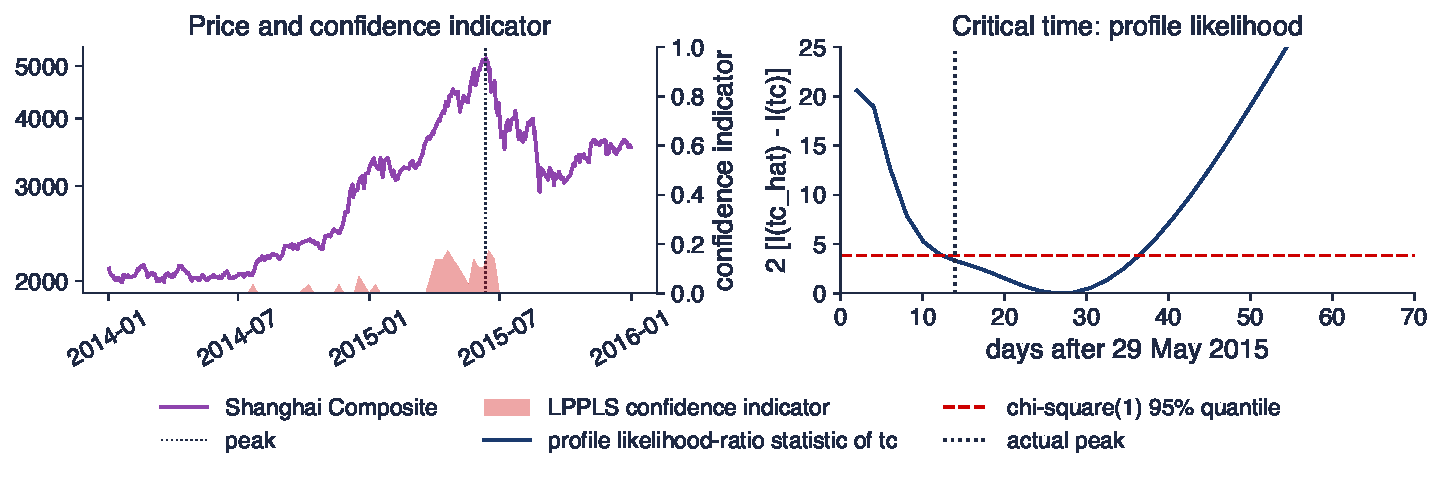
\includegraphics[width=0.97\textwidth,height=0.61\textheight,keepaspectratio]{ats_ch16_lppls.pdf}
\end{center}
\vspace{-0.25cm}
\begin{itemize}
    \item Stînga: indicatorul de încredere în fiecare a cincea zi de tranzacționare; dreapta: verosimilitatea profil a lui $t_c$ pentru fereastra de la minimul din 20 martie 2014 pînă la 29 mai 2015 (293 de zile), ca în analiza în timp real din \refSha
\end{itemize}
\quantlet{ATS\_ch16\_lppls\_inference}{\qlurl{ATS_ch16_lppls_inference}}
\end{frame}

\begin{frame}{Interpretarea ajustării pentru Shanghai}
\itemsize{\small}
\begin{itemize}
    \item Ajustarea care se încheie pe 29 mai 2015 trece de tot filtrul: $m = 0{,}41$, $\omega = 6{,}28$, 5{,}7 oscilații, amortizare 1{,}16; $\hat t_c$ = 24 iunie 2015
    \item Intervalul din verosimilitatea profil: 12 iunie 2015 -- 2 iulie 2015 (20 de zile); maximul din 12 iunie 2015 se află la marginea lui stîngă: o prognoză bună, dar fragilă la alegerea ferestrei
    \item Indicatorul este mic: cel mult 0{,}17 (pe 20 aprilie 2015); puține ferestre se califică simultan, deci indicatorul semnalează un regim, nu o dată
    \item Un succes este o anecdotă: secțiunea următoare numără alarmele pe decenii, cu frecvențele de bază
\end{itemize}
\end{frame}

\begin{frame}{Abordări spectrale ale log-periodicității și critica}
\itemsize{\small}
\begin{itemize}
    \item Oscilația $\cos(\omega\ln(t_c - t))$ este periodică în $\ln(t_c - t)$
    \begin{itemize}
        \item testul: periodograma Lomb a reziduului fără tendință, în funcție de $\ln(t_c - t)$ \refLom
        \item alternativa neparametrică: analiza cu derivata $(H, q)$ \refZS
        \item în timp calendaristic frecvența ei instantanee este $\omega/[2\pi(t_c - t)]$: oscilațiile se accelerează spre $t_c$; transformata Hilbert a reziduului dă direct această fază (instrumentele în \atschlink{https://danpele.github.io/Advanced-Time-Series/RO/Cursuri/capitol11_analiza_spectrala_analiza_wavelet.pdf}{Capitolul 11})
    \end{itemize}
    \item Critica
    \begin{itemize}
        \item vîrfurile log-periodice apar și în zgomot după ajustare și eliminarea tendinței \refFei
        \item prognozele de crah în afara eșantionului sînt slabe \refBJ; estimarea este fragilă \refGF
        \item răspunsuri privind formularea stochastică, filtrele și indicatorii pe multe ferestre: \refSWYZ
    \end{itemize}
    \item O comparație corectă cu PSY folosește aceleași evenimente, date și măsuri de eroare: secțiunea următoare
\end{itemize}
\end{frame}

\begin{frame}{Recapitulare: LPPLS}
\itemsize{\small}
\begin{itemize}
    \item LPPLS modelează creșterea superexponențială cu oscilații log-periodice spre un timp critic; indicatorul de încredere agregă ajustările calificate pe ferestre
    \item Timpul critic cere un interval: verosimilitate profil sau profil modificată; nașterea unei bule se determină mai ușor decît spargerea ei
    \item Testele spectrale ale log-periodicității pot fi păcălite ușor; judecați LPPLS după alarmele lui, nu după ajustări
\end{itemize}
\end{frame}


%=============================================================================
\section{Aplicații cu frecvențe de bază}
%=============================================================================

\begin{frame}{Cinci episoade, un singur protocol}
\itemsize{\footnotesize}
\begin{columns}[T]
\begin{column}{0.34\textwidth}
\centering
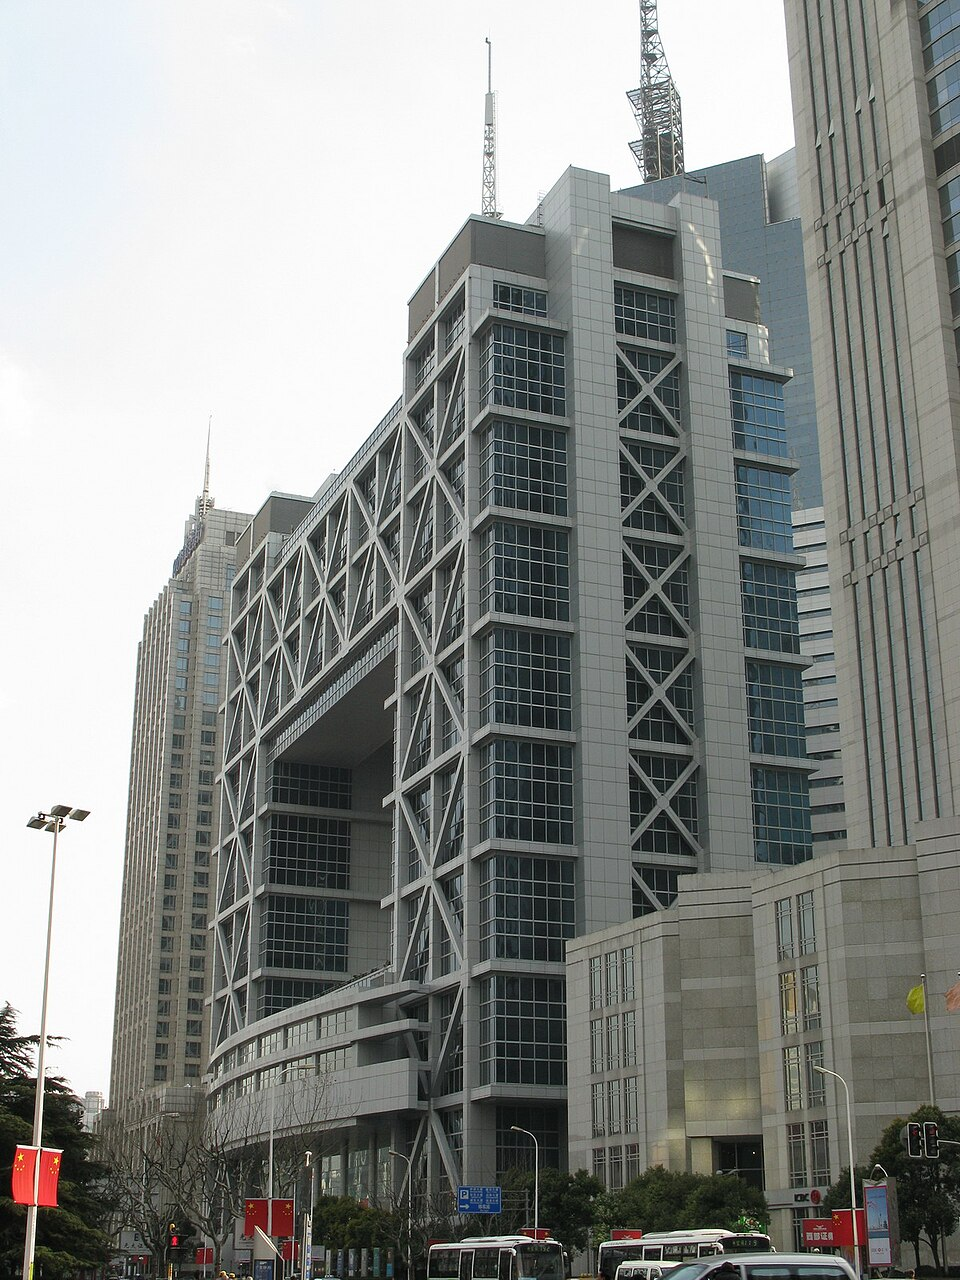
\includegraphics[height=0.4\textheight]{ch16_shanghai_se_2008.jpg}\\[1mm]
\imgcap{Bursa din Shanghai, Pudong, 2008}
\imgcredit{https://commons.wikimedia.org/wiki/File:Shanghai_Stock_Exchange_Building.jpg}{Foto: Baycrest (2008); CC BY-SA 2.5; Wikimedia Commons}
\end{column}
\begin{column}{0.64\textwidth}
\begin{itemize}
    \item Logaritmul prețurilor săptămînale (închiderea de vineri): S\&P 500 și Nasdaq 100 1990--2004, Shanghai Composite 2010--2018, Bitcoin septembrie 2014 -- 2023, BET 2000--2012
    \item Fără laguri; $r_0 = 0{,}01 + 1{,}8/\sqrt T$; durata minimă $\lceil\ln T\rceil$ săptămîni; valori critice Monte Carlo (1000 de traiectorii) și wild bootstrap (499 de extrageri)
    \item Episoade datate cu valori wild punctuale și cu pragul wild de familie pe 52 de săptămîni; data alarmei este data confirmării
    \item Studii de caz: \refPWY{} (Nasdaq), \refPSYa{} (S\&P 500), \refSha{} (Shanghai), \refGDS{} (Bitcoin); pentru BET 2007, vezi și lectura suplimentară \refPMM
\end{itemize}
\end{column}
\end{columns}
\end{frame}

\begin{frame}{BSADF pentru cele cinci episoade}
\itemsize{\footnotesize}
\begin{center}
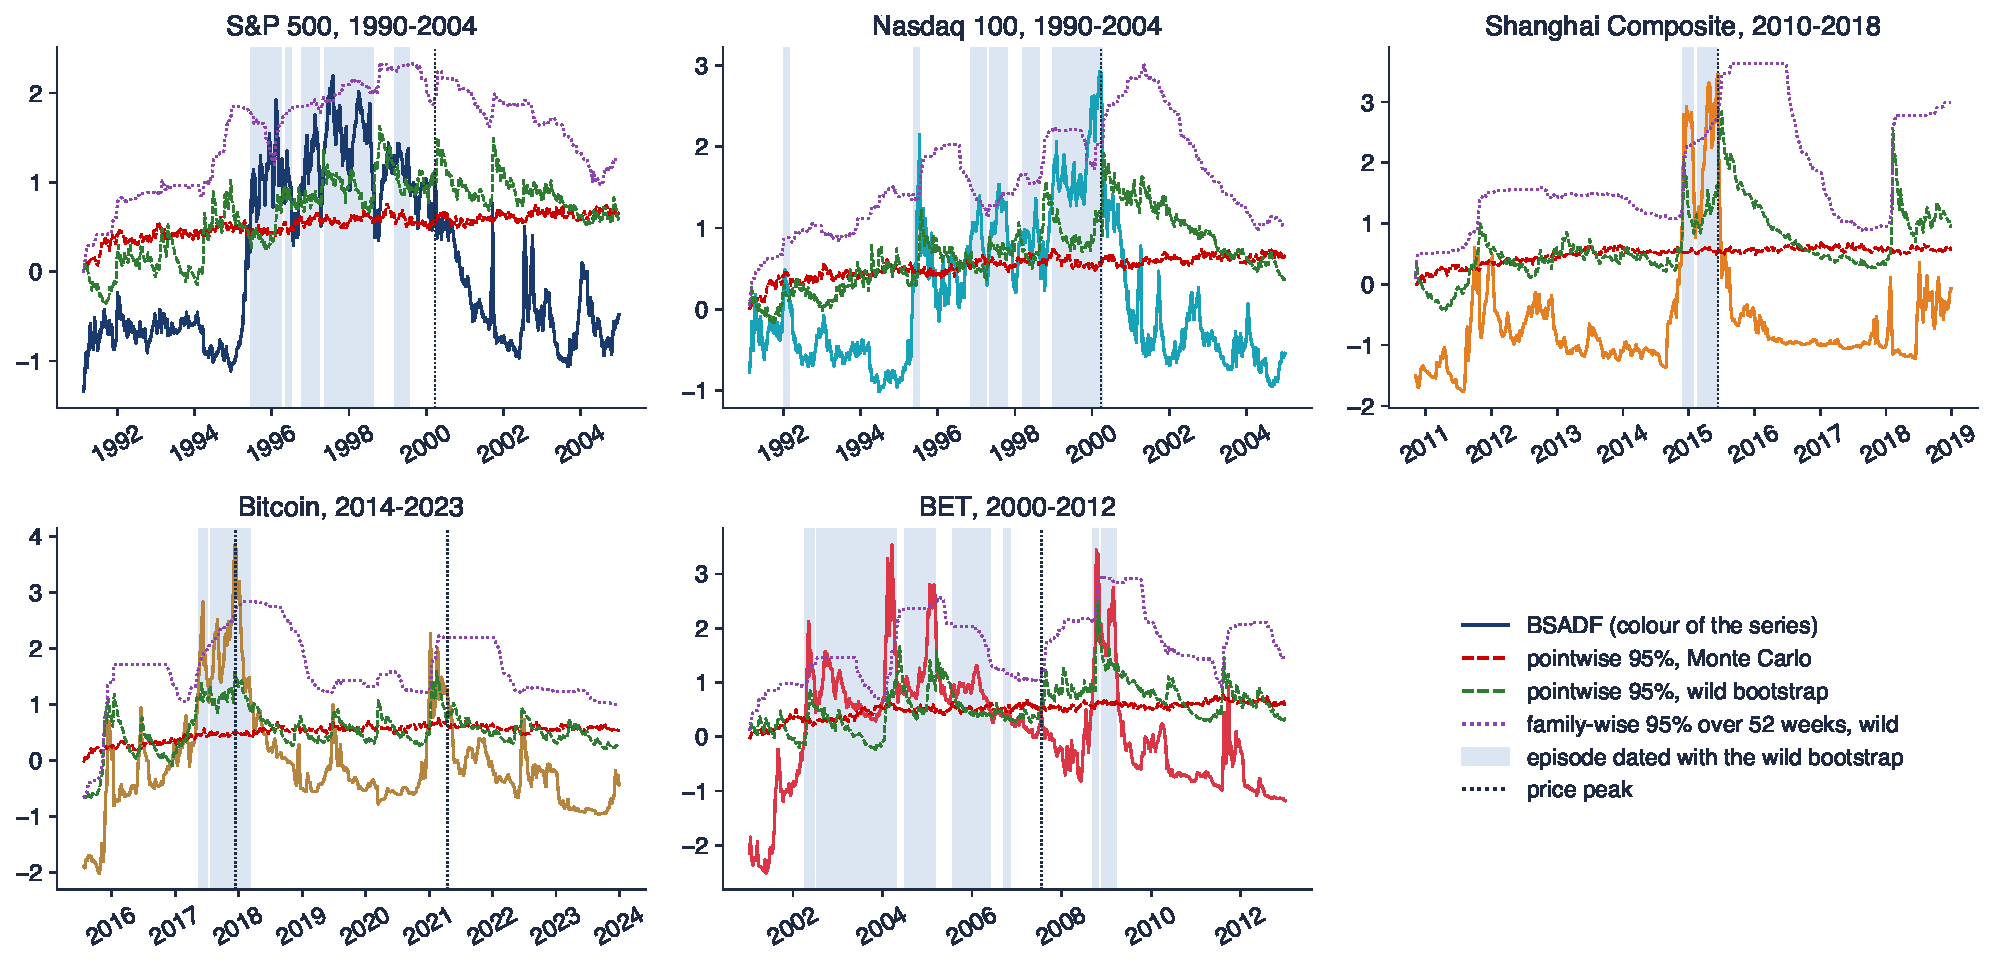
\includegraphics[width=0.97\textwidth,height=0.68\textheight,keepaspectratio]{ats_ch16_episodes.pdf}
\end{center}
\vspace{-0.25cm}
\begin{itemize}
    \item Zonele colorate: episoade datate cu wild bootstrap punctual; liniile verticale punctate: maximele prețurilor
\end{itemize}
\quantlet{ATS\_ch16\_episodes}{\qlurl{ATS_ch16_episodes}}
\end{frame}

\begin{frame}{Interpretarea celor cinci teste}
\itemsize{\footnotesize}
\begin{center}
\scriptsize
\begin{tabular}{lrrrrrr}
\toprule
\textbf{Seria} & $T$ & GSADF & \textbf{vc MC} & \textbf{vc wild} & \textbf{episoade: MC / wild / FW} & \textbf{săptămîni: MC / wild} \\
\midrule
S\&P 500 & 782 & 2{,}19 & 2{,}28 & 2{,}91 & 5 / 6 / 0 & 228 / 167 \\
Nasdaq 100 & 782 & 2{,}92 & 2{,}28 & 3{,}22 & 6 / 6 / 1 & 210 / 159 \\
Shanghai & 460 & 3{,}46 & 2{,}15 & 3{,}90 & 1 / 2 / 1 & 31 / 27 \\
Bitcoin & 484 & 3{,}85 & 2{,}18 & 3{,}15 & 2 / 2 / 1 & 75 / 43 \\
BET & 663 & 3{,}53 & 2{,}29 & 3{,}21 & 3 / 7 / 1 & 213 / 217 \\
\bottomrule
\end{tabular}
\end{center}
\begin{itemize}
    \item S\&P 500: GSADF sub ambele valori critice, totuși datarea punctuală marchează 6 episoade: capcana multiplicității pe date reale; niciun episod de familie
    \item Valorile critice wild depășesc valorile Monte Carlo pentru toate seriile (volatility clustering): Bitcoin și BET resping în continuare; Nasdaq (2{,}92 față de 3{,}22) și Shanghai (3{,}46 față de 3{,}90) nu resping
    \item MC: Monte Carlo; FW: pragul wild de familie pe 52 de săptămîni; vc: valoarea critică de 95\% a GSADF
\end{itemize}
\end{frame}

\begin{frame}{Alarmele dinaintea maximelor}
\itemsize{\footnotesize}
\begin{center}
\scriptsize
\begin{tabular}{lrrrrr}
\toprule
\textbf{Maximul} & \textbf{prima alarmă (2 ani înainte)} & \textbf{avans (săpt.)} & \textbf{activă la maxim} & \textbf{avans FW} & \textbf{scădere în 1 an} \\
\midrule
S\&P 500, 24 martie 2000 & 16 aprilie 1999 & 49 & nu & -- & 25\% \\
Nasdaq 100, 24 martie 2000 & 24 aprilie 1998 & 100 & da & 13 & 65\% \\
Shanghai, 12 iunie 2015 & 9 ianuarie 2015 & 22 & da & 22 & 47\% \\
Bitcoin, 15 decembrie 2017 & 23 iunie 2017 & 25 & da & -- & 82\% \\
Bitcoin, 16 aprilie 2021 & niciuna & -- & nu & -- & 49\% \\
BET, 20 iulie 2007 & 2 septembrie 2005 & 98 & nu & -- & 46\% \\
\bottomrule
\end{tabular}
\end{center}
\begin{itemize}
    \item Fiecare maxim important este precedat de o alarmă punctuală, cu excepția Bitcoin 2021; avansuri între o jumătate de an și doi ani: prea devreme pentru a anticipa un crah, informativ despre regim
    \item BET 2007: alarma din 2 septembrie 2005 este urmată de aproape doi ani de creșteri pînă la maxim și de o scădere de 46\%; controlul de familie elimină majoritatea alarmelor
    \item Numărarea doar a maximelor ascunde alarmele false: alarmele care nu au fost urmate de un crah apar doar cînd evaluăm fiecare dată
\end{itemize}
\end{frame}

\begin{frame}{Valoarea avertizării timpurii pe decenii}
\itemsize{\footnotesize}
\begin{center}
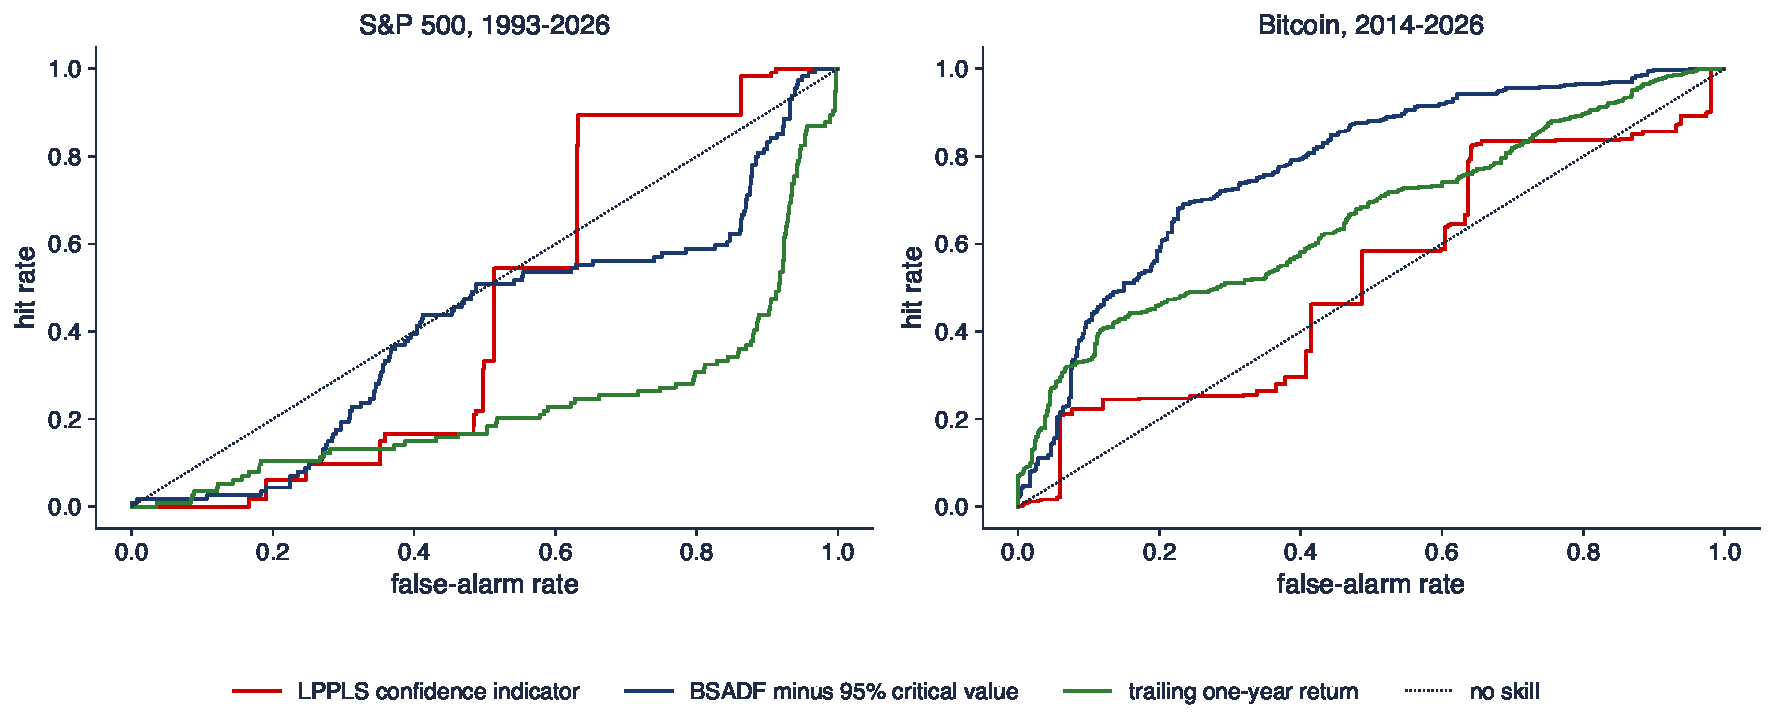
\includegraphics[width=0.97\textwidth,height=0.61\textheight,keepaspectratio]{ats_ch16_evaluation.pdf}
\end{center}
\vspace{-0.25cm}
\begin{itemize}
    \item Evenimentul: o scădere de 20\% în 182 de zile; evaluare în fiecare a cincea zi de tranzacționare (S\&P 500 1\,672 de date, Bitcoin 893); scoruri: indicatorul de încredere LPPLS, BSADF minus valoarea critică punctuală de 95\% (săptămînal, în timp real), randamentul din ultimul an
\end{itemize}
\quantlet{ATS\_ch16\_early\_warning}{\qlurl{ATS_ch16_early_warning}}
\end{frame}

\begin{frame}{Interpretarea evaluării avertizărilor timpurii}
\itemsize{\footnotesize}
\begin{itemize}
    \item Frecvențe de bază: 6{,}8\% dintre datele S\&P 500 și 47{,}6\% dintre datele Bitcoin sînt urmate de o scădere de 20\%: aceeași alarmă înseamnă lucruri foarte diferite pe cele două piețe
    \item S\&P 500, AUC cu intervale block bootstrap de 90\%: indicatorul 0{,}39 [0{,}32; 0{,}48], BSADF 0{,}41 [0{,}28; 0{,}58], momentum 0{,}23 [0{,}10; 0{,}40]: toate sub 0,5
    \item Cele mai multe date S\&P 500 urmate de o scădere de 20\% se află în piețe în declin (2000--2002, 2008), cînd scorurile de exuberanță sînt mici, și puține la vîrful unei creșteri
    \begin{itemize}
        \item deci scorurile sînt \textbf{mai mici} înaintea evenimentelor; alarmele BSADF au precizia 1\%, față de o frecvență de bază de 6{,}8\%
    \end{itemize}
    \item Bitcoin: BSADF are putere predictivă, AUC 0{,}77 [0{,}69; 0{,}85], peste momentum 0{,}66; alarmele lui ating precizia 79\%, față de o frecvență de bază de 47{,}6\% (rata de detecție 32\%, alarme false 8\%)
    \item Indicatorul LPPLS este pozitiv în 35{,}9\% dintre datele S\&P 500 și în 4{,}6\% dintre datele Bitcoin; AUC este 0{,}39 și 0{,}49: în acest protocol nu separă datele dinaintea crahurilor de celelalte
\end{itemize}
\end{frame}

\begin{frame}{Recapitulare: aplicațiile}
\itemsize{\small}
\begin{itemize}
    \item Valorile critice wild bootstrap sînt mai mari decît cele Monte Carlo pe date reale; unele respingeri clasice nu rezistă
    \item Maximele importante sînt de obicei precedate de alarme, dar cu avansuri lungi și variabile; controlul de familie elimină majoritatea lor
    \item Pe decenii, precizia trebuie citită față de frecvența de bază
    \begin{itemize}
        \item scorurile de exuberanță ajută pentru Bitcoin, unde crahurile urmează creșterilor
        \item ele eșuează pentru S\&P 500, unde majoritatea datelor dinaintea crahurilor se află în piețe în declin
    \end{itemize}
\end{itemize}
\end{frame}


%=============================================================================
\section{AI în descoperirea științifică}
%=============================================================================

\begin{frame}{O întrebare deschisă}
\itemsize{\small}
\begin{itemize}
    \item Întrebarea
    \begin{itemize}
        \item conțin alarmele bazate pe rădăcini explozive și pe LPPLS informație despre scăderile mari dincolo de momentum și volatilitate?
        \item după ce ținem seama de frecvențele de bază, de orizonturile suprapuse și de căutarea pe multe active
    \end{itemize}
    \item O formă testabilă
    \begin{itemize}
        \item formal: într-un model logit sau probit al evenimentului pe momentum, volatilitate și scorul alarmei (cu lag), $H_0$: coeficientul alarmei este zero, cu inferență block bootstrap și un panel de active preînregistrat
        \item infirmată de un cîștig semnificativ în afara eșantionului într-o regulă de scor proprie (log score, Brier) față de modelul cu momentum și volatilitate, agregat pe active
    \end{itemize}
    \item Miza
    \begin{itemize}
        \item autoritățile și investitorii citesc indicatorii de bulă ca avertismente
        \item majoritatea dovezilor provin din cîteva episoade celebre, alese după ce s-au produs
        \item literatura de pornire: \refPS, \refAHLST, \refDS, \refBJ, \refHB
    \end{itemize}
\end{itemize}
\end{frame}

\begin{frame}{Bucla de cercetare cu un asistent AI}
\itemsize{\footnotesize}
\begin{itemize}
    \item Un asistent AI (un LLM precum Claude, ChatGPT, Gemini sau Copilot) accelerează fiecare etapă; Semantic Scholar și Elicit ajută la literatură
    \begin{itemize}
        \item \textbf{literatura}: \aiprompt{Listează articole recenzate din 2015 încoace care evaluează detectoarele de bule în afara eșantionului, cu rate ale alarmelor false; dă DOI-urile.} Apoi verificați fiecare DOI și cifrele raportate
        \item \textbf{ipoteza}: \aiprompt{Scrie o preînregistrare: activele, eșantionul, definiția evenimentului, scorurile, modelul de referință, regula de scor, testul și lungimea blocurilor.}
        \item \textbf{cod și replicare}: cereți un BSADF vectorizat; reproduceți întîi o cifră cunoscută (GSADF pentru Nasdaq 100 de aici sau valorile critice PSY)
        \item \textbf{critica}: \aiprompt{Joacă rolul unui recenzent ostil: enumeră toate felurile în care această evaluare ar putea supraestima valoarea alarmelor.}
    \end{itemize}
    \item Raportul: ce s-a cerut, ce s-a păstrat, ce s-a respins (AI\_USE.md, AI\_ERRORS.md)
\end{itemize}
\end{frame}

\begin{frame}{Verificări necesare}
\itemsize{\small}
\begin{itemize}
    \item Fiecare referință există și spune ce se afirmă (DOI-ul funcționează, titlul coincide, rezultatul se află în lucrare)
    \item Coada dreaptă, nu cea stîngă: un ADF scris de un AI folosește adesea valorile critice ale cozii stîngi sau cuantila normală 1,645
    \item Valori critice simulate pentru aceleași $T$, $r_0$, laguri și termeni determiniști; wild bootstrap cînd volatilitatea se schimbă
    \item Fără informație din viitor: fereastra minimă, numărul de laguri și scalarea se stabilesc din datele disponibile la fiecare dată
    \item Multiplicitatea pe date și pe active: ce rată de eroare controlează o bulă raportată?
\end{itemize}
\end{frame}

\begin{frame}{Mini studiu de caz: cîte bule găsește o analiză pe multe active?}
\itemsize{\footnotesize}
\begin{center}
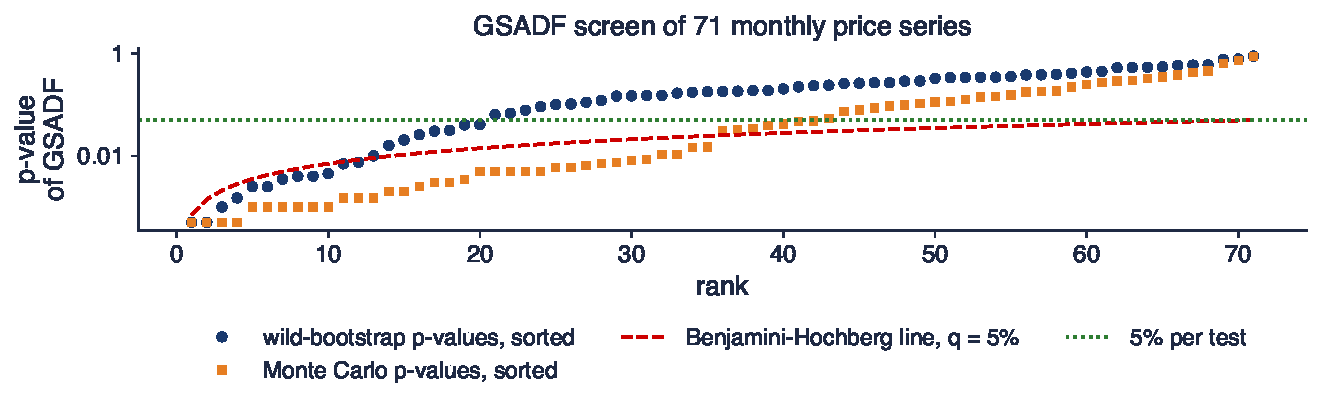
\includegraphics[width=0.97\textwidth,height=0.52\textheight,keepaspectratio]{ats_ch16_ai_case.pdf}
\end{center}
\vspace{-0.25cm}
\begin{itemize}
    \item GSADF pe logaritmul prețului lunar pentru 71 de serii din datele cursului (din 1990 sau din prima lună disponibilă), p-value-uri din 1999 de extrageri wild bootstrap și 1999 Monte Carlo (cel mai mic p-value posibil: 0{,}0005)
    \item Respingeri la 5\%: 42 cu Monte Carlo, 20 cu wild bootstrap (3{,}6 așteptate din întîmplare); după Holm 2, după Benjamini--Hochberg 12. Un rezumat AI precum „bule în 42 dintre active” greșește de două ori: ipoteză nulă greșită și nicio corecție
\end{itemize}
\quantlet{ATS\_ch16\_ai\_screen}{\qlurl{ATS_ch16_ai_screen}}
\end{frame}

\begin{frame}{Idee de proiect}
\itemsize{\small}
\begin{itemize}
    \item \textbf{O evaluare preînregistrată a alarmelor de bulă pe piețele din Europa Centrală și de Est}
    \begin{itemize}
        \item replicați: datarea din \refPSYa{} și wild bootstrap cu control de familie din \refPS{} pe BET, WIG20, BUX, PX și pe rapoartele preț/chirie ale locuințelor (Eurostat)
        \item extindeți: comparați BSADF, monitorizarea cu frontieră și indicatorul LPPLS ca predictori ai scăderilor de 20\%, față de momentum și volatilitate, cu reguli de scor proprii și block bootstrap
        \item preînregistrați: activele, definiția evenimentului, scorurile, orizonturile, testele și regula de decizie, înainte de orice rulare după 1 noiembrie 2026
    \end{itemize}
    \item Livrabilele urmează regulile cursului: repository, raport, AI\_USE.md, AI\_ERRORS.md, susținere orală
\end{itemize}
\end{frame}


%=============================================================================
\section{Încheiere}
%=============================================================================

\begin{frame}{Idei de reținut}
\itemsize{\small}
\begin{itemize}
    \item O bulă rațională este o componentă autoregresivă explozivă; nu poate fi negativă și nu poate apărea ulterior, iar prăbușirile periodice o ascund de testele pe tot eșantionul
    \item Rădăcinile explozive se învață cu rată exponențială, cu limite Cauchy; asimptotica ușor explozivă este invariantă și justifică testele pe ferestre
    \item Valorile critice trebuie să corespundă designului; wild bootstrap tratează volatilitatea variabilă; datarea cere controlul erorii de familie
    \item Începuturile datate sînt tîrzii, alarmele sînt timpurii față de maxime, iar precizia depinde de frecvența de bază
    \item Testați fundamentele, nu doar prețurile; judecați LPPLS și PSY după aceleași alarme, evenimente și scoruri
\end{itemize}
\end{frame}

\begin{frame}{Formule de reținut}
\itemsize{\small}
{\renewcommand{\arraystretch}{1.4}\begin{center}
\footnotesize
\begin{tabular}{ll}
\toprule
\textbf{Obiectul} & \textbf{Formula} \\
\midrule
Bula & $P_t = F_t + B_t$, $\E_t B_{t+1} = (1 + r)B_t$ \\
Fundamentul, dividende mers aleator & $F_t = D_t/r + \mu(1 + r)/r^2$ \\
Limita OLS explozivă & $\rho^n(\hat\rho - \rho)/(\rho^2 - 1) \Rightarrow \mathcal C$ \\
Statisticile recursive & $\mathrm{BSADF}_{r_2} = \sup_{r_1}\mathrm{ADF}_{r_1}^{r_2}$, $\mathrm{GSADF} = \sup_{r_2}\mathrm{BSADF}_{r_2}$ \\
Fereastra minimă & $r_0 = 0{,}01 + 1{,}8/\sqrt T$ \\
Frontiera de monitorizare & $b_t = \sqrt{\tfrac{t - n}{n}\tfrac{t}{n}[a^2 + \ln\tfrac{t}{t - n}]}$, $1 - \Phi(a) + a\varphi(a) = \alpha$ \\
Precizia unei alarme & $H\pi_0/[H\pi_0 + F(1 - \pi_0)]$ \\
LPPLS & $\ln p = A + B f + C_1 f\cos(\omega\ln(t_c - t)) + C_2 f\sin(\omega\ln(t_c - t))$, $f = (t_c - t)^m$ \\
\bottomrule
\end{tabular}
\end{center}
}
\end{frame}

\begin{frame}{Autoevaluare (1/2)}
\itemsize{\small}
\begin{itemize}
    \item Derivați $F_t$ cînd dividendele urmează $D_t = \mu + D_{t-1} + \varepsilon_t$; cît este $F_t$ pentru $r = 0{,}04$, $\mu = 0{,}1$, $D_t = 3$?
    \item De ce nu poate o bulă rațională să apară după prima zi de tranzacționare?
    \item De ce eșuează ADF pe tot eșantionul în fața unei bule Evans?
    \item De ce este limita lui $\hat\rho$ pentru o rădăcină explozivă fixă Cauchy doar cu erori gaussiene?
    \item Un eșantion are $T = 400$ de săptămîni. Cît sînt $r_0$ și fereastra minimă?
    \item De ce este valoarea critică GSADF mai mare decît cea SADF?
\end{itemize}
\end{frame}

\begin{frame}{Autoevaluare (2/2)}
\itemsize{\small}
\begin{itemize}
    \item Ce păstrează wild bootstrap din date și ce elimină?
    \item O alarmă are $H = 0{,}7$ și $F = 0{,}1$; frecvența de bază este 4\%. Cît este precizia ei?
    \item De ce trebuie ca data alarmei să fie data confirmării și nu începutul datat?
    \item Raportul preț/chirie este exploziv, iar chiriile reale sînt și ele explozive. Ce concluzie trageți?
    \item De ce este prea îngust un interval din verosimilitatea profil pentru $t_c$ cu reziduuri autocorelate?
    \item O analiză pe 80 de active găsește 20 de respingeri GSADF la 5\%. Care sînt primele două verificări?
\end{itemize}
\end{frame}

\begin{frame}{Autoevaluare: răspunsuri (1/2)}
\itemsize{\small}
\begin{itemize}
    \item $F_t = D_t/r + \mu(1 + r)/r^2 = 75 + 65 = 140$
    \item Dacă $B_t = 0$, atunci $\E_t B_{t+1} = 0$ și $B_{t+1} \ge 0$ (nu există bule negative), deci $B_{t+1} = 0$ aproape sigur; prin inducție, bula rămîne zero
    \item Prăbușirile împerechează cele mai mari scăderi cu cele mai mari niveluri și trag panta OLS în jos; pe tot eșantionul seria arată I(1) sau staționară
    \item $\rho^n(\hat\rho - \rho)/(\rho^2 - 1) \approx X_n/Y_n$, cu $X_n$, $Y_n$ dominate de cîteva șocuri: sînt normale doar dacă șocurile sînt normale; nicio teoremă limită centrală nu acționează în interiorul lor
    \item $r_0 = 0{,}01 + 1{,}8/20 = 0{,}1$; fereastra minimă $\lfloor 0{,}1 \cdot 400\rfloor = 40$ de săptămîni
    \item GSADF ia supremul pe mai multe ferestre (toate începuturile și sfîrșiturile), deci sub ipoteza nulă maximul lui este mai mare
\end{itemize}
\end{frame}

\begin{frame}{Autoevaluare: răspunsuri (2/2)}
\itemsize{\small}
\begin{itemize}
    \item Păstrează tiparul volatilității $|\hat e_t|$ (și dinamica pe termen scurt a modelului nul); semnele aleatoare elimină orice componentă explozivă sau predictibilă
    \item $0{,}7 \cdot 0{,}04/(0{,}7 \cdot 0{,}04 + 0{,}1 \cdot 0{,}96) = 0{,}028/0{,}124 \approx 0{,}23$
    \item Începutul este cunoscut doar după numărul minim de depășiri; folosirea lui ca dată a alarmei ar folosi informație din viitor
    \item Aceste teste nu arată o bulă: fundamentul explică accelerarea; ar trebui testat dacă raportul explodează peste ce implică chiriile
    \item Reziduurile autocorelate conțin mai puțină informație decît $n$ erori independente, iar parametrii de deranj sînt ignorați: verosimilitatea este prea ascuțită
    \item Dacă valorile critice țin seama de volatilitatea variabilă (wild bootstrap); dacă numărul respingerilor rezistă unei corecții pentru testare multiplă (4 sînt așteptate din întîmplare)
\end{itemize}
\end{frame}

\begin{frame}{Lecturi suplimentare și legături}
\itemsize{\small}
\begin{columns}[T]
\begin{column}{0.34\textwidth}
\centering
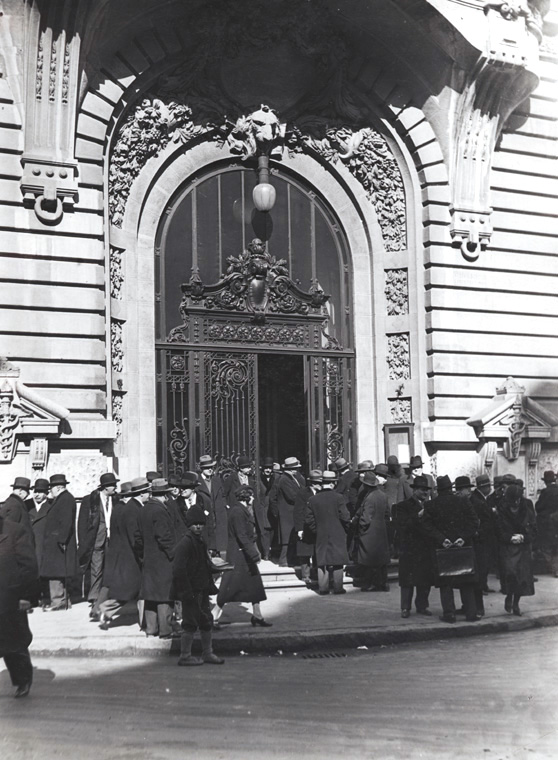
\includegraphics[height=0.4\textheight]{ch16_bvb_palace_1928.jpg}\\[1mm]
\imgcap{Palatul Bursei din București, martie 1928}
\imgcredit{https://commons.wikimedia.org/wiki/File:Nicolae_Ionescu_-_The_Stock_Exchange_Palace_in_March_1928.jpg}{Foto: Nicolae Ionescu (1928); public domain; Wikimedia Commons}
\end{column}
\begin{column}{0.64\textwidth}
\begin{itemize}
    \item Sinteze
    \begin{itemize}
        \item \refGur; \refShi; \refKA
        \item bulele și randamentele ulterioare: \refGSY
    \end{itemize}
    \item Implementare: pachetul R \texttt{exuber} \refVPM
    \begin{itemize}
        \item Quantlet-urile noastre reproduc statisticile lui în Python
    \end{itemize}
    \item Aplicații pe piețe, în risc și politici: \atschlink{https://danpele.github.io/MFM/RO/Cursuri/capitol17_bule_crahuri.pdf}{MFM, Capitolul 17}
    \item Lectură suplimentară despre Bursa de Valori București: \refPMM
    \item Cursul se încheie aici; susținerea proiectelor este descrisă în \atschlink{https://danpele.github.io/Advanced-Time-Series/RO/Cursuri/capitol15_recapitulare_proiecte.pdf}{Capitolul 15}
\end{itemize}
\end{column}
\end{columns}
\end{frame}


%=============================================================================
\section{Anexă}
%=============================================================================

\begin{frame}{Anexă: limita Cauchy în cazul ușor exploziv}
\hypertarget{atsapp1}{}\atsappback{atssrc1}{Înapoi}
\itemsize{\small}
\begin{itemize}
    \item $\rho_n = 1 + c/k_n$; $X_n = k_n^{-1/2}\sum_{j=1}^{n}\rho_n^{-(n-j)-1}u_j$, $Y_n = k_n^{-1/2}\sum_{j=1}^{n}\rho_n^{-j}u_j$; ponderile $\rho_n^{-j} \approx e^{-cj/k_n}$ scad pe $O(k_n)$ termeni
    \item Lindeberg: nicio pondere nu domină, deci $(X_n, Y_n) \Rightarrow (X, Y)$, independente $N(0, \sigma^2/2c)$ ($\sum_j\rho_n^{-2j} \approx k_n/2c$); independența vine din faptul că $X_n$ și $Y_n$ se sprijină pe cele două capete ale eșantionului și $k_n = o(n)$
    \item $(k_n\rho_n^n)^{-2}\sum_t y_{t-1}^2 \Rightarrow Y^2/2c$ și $(k_n\rho_n^n)^{-1}\sum_t y_{t-1}u_t \Rightarrow XY$, deci $\dfrac{k_n\rho_n^n}{2c}(\hat\rho - \rho_n) \Rightarrow X/Y \sim \mathcal C$ \refPM
    \item Raportul a două normale centrate independente cu dispersii egale este Cauchy standard: $X/Y = \tan\Theta$, cu $\Theta$ uniform pe $(-\pi/2, \pi/2)$
\end{itemize}
\end{frame}

\begin{frame}{Anexă: frontiera de monitorizare}
\hypertarget{atsapp2}{}\atsappback{atssrc2}{Înapoi}
\itemsize{\small}
\begin{itemize}
    \item Sub ipoteza nulă, $S_t \approx n^{-1/2}\sigma^{-1}[\sum_{j \le t}\varepsilon_j - (t/n)\sum_{j \le n}\varepsilon_j]$; cu $s = (t - n)/n$: $S \Rightarrow Z(s) = W(1 + s) - (1 + s)W(1)$, $\Var Z(s) = s(1 + s)$
    \item Inversarea timpului: $Z(s) = s\,B(1 + 1/s)$ pentru o mișcare browniană standard $B$; cu $u = 1/s$, evenimentul $Z(s) > \sqrt{s(1 + s)[a^2 + \ln((1 + s)/s)]}$ devine $B(1 + u) > \sqrt{(1 + u)[a^2 + \ln(1 + u)]}$
    \item Robbins--Siegmund: $\Pr\{B(1 + u) > \sqrt{(1 + u)[a^2 + \ln(1 + u)]}$ pentru un $u \ge 0\} = 1 - \Phi(a) + a\varphi(a)$; versiunea bilaterală o dublează, forma folosită de \refCSW
    \item În $t$: $s(1 + s) = \frac{t - n}{n}\cdot\frac{t}{n}$ și $(1 + s)/s = t/(t - n)$, de unde rezultă $b_t$; un orizont finit face testul conservator
\end{itemize}
\end{frame}


%=============================================================================
\section{Bibliografie}
%=============================================================================

\begin{frame}{Bibliografie (1/4)}
\itemsize{\tiny}
\begin{itemize}
    \item Anderson, T. W. (1959). On asymptotic distributions of estimates of parameters of stochastic difference equations. \textit{The Annals of Mathematical Statistics}, 30(3), 676--687. \href{https://doi.org/10.1214/aoms/1177706198}{doi:10.1214/aoms/1177706198}
    \item Astill, S., Harvey, D. I., Leybourne, S. J., Sollis, R., \& Taylor, A. M. R. (2018). Real-time monitoring for explosive financial bubbles. \textit{Journal of Time Series Analysis}, 39(6), 863--891. \href{https://doi.org/10.1111/jtsa.12409}{doi:10.1111/jtsa.12409}
    \item Astill, S., Harvey, D. I., Leybourne, S. J., \& Taylor, A. M. R. (2017). Tests for an end-of-sample bubble in financial time series. \textit{Econometric Reviews}, 36(6--9), 651--666. \href{https://doi.org/10.1080/07474938.2017.1307490}{doi:10.1080/07474938.2017.1307490}
    \item Blanchard, O. J., \& Watson, M. W. (1982). Bubbles, rational expectations and financial markets. NBER Working Paper 945. \href{https://doi.org/10.3386/w0945}{doi:10.3386/w0945}
    \item Brée, D. S., \& Joseph, N. L. (2013). Testing for financial crashes using the log periodic power law model. \textit{International Review of Financial Analysis}, 30, 287--297. \href{https://doi.org/10.1016/j.irfa.2013.05.005}{doi:10.1016/j.irfa.2013.05.005}
    \item Campbell, J. Y., \& Shiller, R. J. (1987). Cointegration and tests of present value models. \textit{Journal of Political Economy}, 95(5), 1062--1088. \href{https://doi.org/10.1086/261502}{doi:10.1086/261502}
    \item Chu, C.-S. J., Stinchcombe, M., \& White, H. (1996). Monitoring structural change. \textit{Econometrica}, 64(5), 1045--1065. \href{https://doi.org/10.2307/2171955}{doi:10.2307/2171955}
    \item Demos, G., \& Sornette, D. (2017). Birth or burst of financial bubbles: Which one is easier to diagnose? \textit{Quantitative Finance}, 17(5), 657--675. \href{https://doi.org/10.1080/14697688.2016.1231417}{doi:10.1080/14697688.2016.1231417}
    \item Diba, B. T., \& Grossman, H. I. (1988a). The theory of rational bubbles in stock prices. \textit{The Economic Journal}, 98(392), 746--754. \href{https://doi.org/10.2307/2233912}{doi:10.2307/2233912}
    \item Diba, B. T., \& Grossman, H. I. (1988b). Explosive rational bubbles in stock prices? \textit{American Economic Review}, 78(3), 520--530. \href{https://ideas.repec.org/a/aea/aecrev/v78y1988i3p520-30.html}{ideas.repec.org}
    \item Dickey, D. A., \& Fuller, W. A. (1979). Distribution of the estimators for autoregressive time series with a unit root. \textit{Journal of the American Statistical Association}, 74(366), 427--431. \href{https://doi.org/10.1080/01621459.1979.10482531}{doi:10.1080/01621459.1979.10482531}
    \item Evans, G. W. (1991). Pitfalls in testing for explosive bubbles in asset prices. \textit{American Economic Review}, 81(4), 922--930. \href{https://ideas.repec.org/a/aea/aecrev/v81y1991i4p922-30.html}{ideas.repec.org}
\end{itemize}
\end{frame}

\begin{frame}{Bibliografie (2/4)}
\itemsize{\tiny}
\begin{itemize}
    \item Feigenbaum, J. A. (2001). A statistical analysis of log-periodic precursors to financial crashes. \textit{Quantitative Finance}, 1(3), 346--360. \href{https://doi.org/10.1088/1469-7688/1/3/306}{doi:10.1088/1469-7688/1/3/306}
    \item Filimonov, V., Demos, G., \& Sornette, D. (2017). Modified profile likelihood inference and interval forecast of the burst of financial bubbles. \textit{Quantitative Finance}, 17(8), 1167--1186. \href{https://doi.org/10.1080/14697688.2016.1276298}{doi:10.1080/14697688.2016.1276298}
    \item Filimonov, V., \& Sornette, D. (2013). A stable and robust calibration scheme of the log-periodic power law model. \textit{Physica A}, 392(17), 3698--3707. \href{https://doi.org/10.1016/j.physa.2013.04.012}{doi:10.1016/j.physa.2013.04.012}
    \item Geraskin, P., \& Fantazzini, D. (2013). Everything you always wanted to know about log-periodic power laws for bubble modeling but were afraid to ask. \textit{The European Journal of Finance}, 19(5), 366--391. \href{https://doi.org/10.1080/1351847X.2011.601657}{doi:10.1080/1351847X.2011.601657}
    \item Gerlach, J.-C., Demos, G., \& Sornette, D. (2019). Dissection of Bitcoin\textquoteright s multiscale bubble history from January 2012 to February 2018. \textit{Royal Society Open Science}, 6(7), 180643. \href{https://doi.org/10.1098/rsos.180643}{doi:10.1098/rsos.180643}
    \item Greenwood, R., Shleifer, A., \& You, Y. (2019). Bubbles for Fama. \textit{Journal of Financial Economics}, 131(1), 20--43. \href{https://doi.org/10.1016/j.jfineco.2018.09.002}{doi:10.1016/j.jfineco.2018.09.002}
    \item Gürkaynak, R. S. (2008). Econometric tests of asset price bubbles: Taking stock. \textit{Journal of Economic Surveys}, 22(1), 166--186. \href{https://doi.org/10.1111/j.1467-6419.2007.00530.x}{doi:10.1111/j.1467-6419.2007.00530.x}
    \item Hamilton, J. D. (1994). \textit{Time Series Analysis}. Princeton University Press. \href{https://doi.org/10.1515/9780691218632}{doi:10.1515/9780691218632}
    \item Harvey, D. I., Leybourne, S. J., \& Sollis, R. (2017). Improving the accuracy of asset price bubble start and end date estimators. \textit{Journal of Empirical Finance}, 40, 121--138. \href{https://doi.org/10.1016/j.jempfin.2016.11.001}{doi:10.1016/j.jempfin.2016.11.001}
    \item Harvey, D. I., Leybourne, S. J., Sollis, R., \& Taylor, A. M. R. (2016). Tests for explosive financial bubbles in the presence of non-stationary volatility. \textit{Journal of Empirical Finance}, 38, 548--574. \href{https://doi.org/10.1016/j.jempfin.2015.09.002}{doi:10.1016/j.jempfin.2015.09.002}
    \item Harvey, D. I., Leybourne, S. J., \& Zu, Y. (2020). Sign-based unit root tests for explosive financial bubbles in the presence of deterministically time-varying volatility. \textit{Econometric Theory}, 36(1), 122--169. \href{https://doi.org/10.1017/S0266466619000057}{doi:10.1017/S0266466619000057}
    \item Homm, U., \& Breitung, J. (2012). Testing for speculative bubbles in stock markets: A comparison of alternative methods. \textit{Journal of Financial Econometrics}, 10(1), 198--231. \href{https://doi.org/10.1093/jjfinec/nbr009}{doi:10.1093/jjfinec/nbr009}
\end{itemize}
\end{frame}

\begin{frame}{Bibliografie (3/4)}
\itemsize{\tiny}
\begin{itemize}
    \item Johansen, A., Ledoit, O., \& Sornette, D. (2000). Crashes as critical points. \textit{International Journal of Theoretical and Applied Finance}, 3(2), 219--255. \href{https://doi.org/10.1142/S0219024900000115}{doi:10.1142/S0219024900000115}
    \item Kaminsky, G., Lizondo, S., \& Reinhart, C. M. (1998). Leading indicators of currency crises. \textit{IMF Staff Papers}, 45(1), 1--48. \href{https://doi.org/10.2307/3867328}{doi:10.2307/3867328}
    \item Kindleberger, C. P., \& Aliber, R. Z. (2005). \textit{Manias, Panics and Crashes: A History of Financial Crises} (5th ed.). Palgrave Macmillan. \href{https://doi.org/10.1057/9780230628045}{doi:10.1057/9780230628045}
    \item Lomb, N. R. (1976). Least-squares frequency analysis of unequally spaced data. \textit{Astrophysics and Space Science}, 39(2), 447--462. \href{https://doi.org/10.1007/BF00648343}{doi:10.1007/BF00648343}
    \item Pavlidis, E., Yusupova, A., Paya, I., Peel, D., Martínez-García, E., Mack, A., \& Grossman, V. (2016). Episodes of exuberance in housing markets: In search of the smoking gun. \textit{The Journal of Real Estate Finance and Economics}, 53(4), 419--449. \href{https://doi.org/10.1007/s11146-015-9531-2}{doi:10.1007/s11146-015-9531-2}
    \item Pele, D. T., \& Mazurencu-Marinescu, M. (2012). Modelling stock market crashes: The case of Bucharest Stock Exchange. \textit{Procedia -- Social and Behavioral Sciences}, 58, 533--542 (further reading). \href{https://doi.org/10.1016/j.sbspro.2012.09.1030}{doi:10.1016/j.sbspro.2012.09.1030}
    \item Phillips, P. C. B., \& Magdalinos, T. (2007). Limit theory for moderate deviations from a unit root. \textit{Journal of Econometrics}, 136(1), 115--130. \href{https://doi.org/10.1016/j.jeconom.2005.08.002}{doi:10.1016/j.jeconom.2005.08.002}
    \item Phillips, P. C. B., \& Shi, S. (2018). Financial bubble implosion and reverse regression. \textit{Econometric Theory}, 34(4), 705--753. \href{https://doi.org/10.1017/S0266466617000202}{doi:10.1017/S0266466617000202}
    \item Phillips, P. C. B., \& Shi, S. (2020). Real time monitoring of asset markets: Bubbles and crises. In \textit{Handbook of Statistics}, Vol.\ 42, 61--80. Elsevier. \href{https://doi.org/10.1016/bs.host.2018.12.002}{doi:10.1016/bs.host.2018.12.002}
    \item Phillips, P. C. B., Shi, S., \& Yu, J. (2015a). Testing for multiple bubbles: Historical episodes of exuberance and collapse in the S\&P 500. \textit{International Economic Review}, 56(4), 1043--1078. \href{https://doi.org/10.1111/iere.12132}{doi:10.1111/iere.12132}
    \item Phillips, P. C. B., Shi, S., \& Yu, J. (2015b). Testing for multiple bubbles: Limit theory of real-time detectors. \textit{International Economic Review}, 56(4), 1079--1134. \href{https://doi.org/10.1111/iere.12131}{doi:10.1111/iere.12131}
    \item Phillips, P. C. B., Shi, S., \& Yu, J. (2014). Specification sensitivity in right-tailed unit root testing for explosive behaviour. \textit{Oxford Bulletin of Economics and Statistics}, 76(3), 315--333. \href{https://doi.org/10.1111/obes.12026}{doi:10.1111/obes.12026}
\end{itemize}
\end{frame}

\begin{frame}{Bibliografie (4/4)}
\itemsize{\tiny}
\begin{itemize}
    \item Phillips, P. C. B., Wu, Y., \& Yu, J. (2011). Explosive behavior in the 1990s Nasdaq: When did exuberance escalate asset values? \textit{International Economic Review}, 52(1), 201--226. \href{https://doi.org/10.1111/j.1468-2354.2010.00625.x}{doi:10.1111/j.1468-2354.2010.00625.x}
    \item Phillips, P. C. B., \& Yu, J. (2011). Dating the timeline of financial bubbles during the subprime crisis. \textit{Quantitative Economics}, 2(3), 455--491. \href{https://doi.org/10.3982/QE82}{doi:10.3982/QE82}
    \item Santos, M. S., \& Woodford, M. (1997). Rational asset pricing bubbles. \textit{Econometrica}, 65(1), 19--57. \href{https://doi.org/10.2307/2171812}{doi:10.2307/2171812}
    \item Shiller, R. J. (2015). \textit{Irrational Exuberance} (3rd ed.). Princeton University Press. \href{https://doi.org/10.1515/9781400865536}{doi:10.1515/9781400865536}
    \item Shu, M., \& Zhu, W. (2020). Detection of Chinese stock market bubbles with LPPLS confidence indicator. \textit{Physica A}, 557, 124892. \href{https://doi.org/10.1016/j.physa.2020.124892}{doi:10.1016/j.physa.2020.124892}
    \item Sornette, D., Demos, G., Zhang, Q., Cauwels, P., \& Zhang, Q. (2015). Real-time prediction and post-mortem analysis of the Shanghai 2015 stock market bubble and crash. \textit{Journal of Investment Strategies}, 4(4), 77--95. \href{https://doi.org/10.21314/JOIS.2015.063}{doi:10.21314/JOIS.2015.063}
    \item Sornette, D., Woodard, R., Yan, W., \& Zhou, W.-X. (2013). Clarifications to questions and criticisms on the Johansen--Ledoit--Sornette financial bubble model. \textit{Physica A}, 392(19), 4417--4428. \href{https://doi.org/10.1016/j.physa.2013.05.011}{doi:10.1016/j.physa.2013.05.011}
    \item Tirole, J. (1985). Asset bubbles and overlapping generations. \textit{Econometrica}, 53(6), 1499--1528. \href{https://doi.org/10.2307/1913232}{doi:10.2307/1913232}
    \item Vasilopoulos, K., Pavlidis, E., \& Martínez-García, E. (2022). exuber: Recursive right-tailed unit root testing with R. \textit{Journal of Statistical Software}, 103(10). \href{https://doi.org/10.18637/jss.v103.i10}{doi:10.18637/jss.v103.i10}
    \item White, J. S. (1958). The limiting distribution of the serial correlation coefficient in the explosive case. \textit{The Annals of Mathematical Statistics}, 29(4), 1188--1197. \href{https://doi.org/10.1214/aoms/1177706450}{doi:10.1214/aoms/1177706450}
    \item Zhou, W.-X., \& Sornette, D. (2003). Nonparametric analyses of log-periodic precursors to financial crashes. \textit{International Journal of Modern Physics C}, 14(8), 1107--1125. \href{https://doi.org/10.1142/S0129183103005212}{doi:10.1142/S0129183103005212}
\end{itemize}
\end{frame}

\end{document}
